%\documentclass[handout]{beamer}
\documentclass[]{beamer}
\mode<presentation>
\usepackage{beamerthemesplit}
\usepackage{subfigure}
\usepackage{slashed}
\usepackage{color}
%\usepackage{pdffig}
\usepackage{pgf}
\usepackage{amsmath}
\usepackage{graphics}
\usepackage{graphicx}
\usepackage{fancybox}
\usepackage{subfigure}
\usepackage{multirow}
\usepackage{sidecap} 
\usepackage{psfrag}
\usepackage{rotating}
\usepackage{amsmath}
\usepackage{tcolorbox}
\usepackage{tikz}
\usepackage{epstopdf}
\usepackage{wasysym}
\usepackage[normalem]{ulem}

\makeatletter
\def\UL@putbox{\ifx\UL@start\@empty \else % not inner
  \vrule\@width\z@ \LA@penalty\@M
  {\UL@skip\wd\UL@box \UL@leaders \kern-\UL@skip}%
    \phantom{\box\UL@box}%
  \fi}
\makeatother

% Variable width alert block
\newenvironment<>{varalertblock}[2][0.9\textwidth]{%
	\setlength{\textwidth}{#1}%
	\setlength{\linewidth}{\textwidth}%
	\begin{actionenv}#3%
		\def\insertblocktitle{#2}%
		\par%
		\setbeamercolor{block body}{bg=green,fg=red}
		%\setbeamercolor{local structure}{parent=alerted text}%
		\usebeamertemplate{block alerted begin}}
	{\par%
		\usebeamertemplate{block alerted end}%
\end{actionenv}}


\definecolor{ah1col}{rgb}{0.84, 0.84, 0.84}
\setbeamertemplate{navigation symbols}{}
\renewcommand{\insertnavigation}[1]{}

%\usetheme{AnnArbor}
\usetheme{CambridgeUS}

%\setbeamertemplate{headline}{}
%\setbeamercolor{palette primary}{fg=yellow, bg=black}
%\setbeamercolor{palette secondary}{fg=black, bg=white}
%\setbeamercolor{palette tertiary}{fg=yellow, bg=green}


% Uncomment these to make handouts
%\usepackage{pgfpages}
%\pgfpagesuselayout{4 on 1}[a4paper, border shrink=5mm]
%\usetheme{default}

%Font and colour commands
\usefonttheme[onlylarge]{structuresmallcapsserif}
\usefonttheme[onlysmall]{structurebold}
\setbeamerfont{title}{shape=\itshape,family=\rmfamily}
%\setbeamercolor{title}{fg=red!80!black, bg=red!20!white}
\setbeamercolor{title}{fg=yellow, bg=black}
%\setbeamercolor{block body}{bg=black, fg=white}
%\usepackage{palatino}
%\usepackage{charter}
%\sffamily
%bf

%Uncomment this to make unshown listings slightly
%visible
%\setbeamercovered{transparent}


%\title[{\tt DPF'13, UCSC}]{Exclusive $B\to X_{\{c,u\}} \ell^- \bar{\nu}$ angular analyses \\with hadronic tagging from $\babar$}
%\title[]{Right-handed weak charged currents via exclusive \\ $\Bbar\to X_{\{c,u\}} \ell^- \bar{\nu}_\ell$ angular analyses \\with hadronic tagging from $\babar$}
\title[{\tt CODEX-b, $3^{rd}$ LLP LHC workshop, CERN}]{{\LARGE LLP seaches with CODEX-b\\ {\rm {\small CO\textcolor{white}{mpact} D\textcolor{white}{etector for} EX\textcolor{white}{otics} \textcolor{white}{at LHC}b}}} \\ {\small {\tt \textcolor{white}{[1708.09395]}}}  }
%\title[{\tt Physik-Institut, UZH}]{Right-handed weak charged currents via exclusive \\ $\Bbar\to X_{\{c,u\}} \ell^- \bar{\nu}_\ell$ angular analyses \\with hadronic tagging from $\babar$}

\date[May $18^{th}$, 2018]{{\tt {\small Third workshop of the LHC LLP Community,\\ May  $16^{th}$-$18^{th}$ 2018, CERN}}}
%\date[Nov. $26^{th}$, 2013]{{\tt Physik-Institut, UZH, Nov. $26^{th}$, 2013}}}

%\subtitle[]{(BAD \# 2566)}

\author[Biplab Dey]{\vspace{0.5cm}{\LARGE Biplab~Dey}\vspace{0.1cm}\\ {\large on behalf of the CODEX-b WG}}

\institute[]{
%\vspace{-0.9cm}

{\flushbottom
 %\hspace{-1cm}
\includegraphics[width=1.7in]{figs/logos/uzh_logo.jpg}\hspace{0.5cm} 
 %
\includegraphics[width=0.75in]{figs/logos/lhcb_logo-300dpi.jpg} \hspace{1cm}
 %
\includegraphics[width=1.0in]{figs/logos/lhcb_logo-300dpi.jpg} \hspace{6cm}
 %
\includegraphics[width=0.7in]{figs/logos/infn_logo.jpeg}
 
\includegraphics[width=0.5in]{figs/logos/ccnu.jpg}
% 
\includegraphics[width=0.9in]{figs/logos/SLAC_Logo.jpg}\hspace{1.6cm}
% 
\includegraphics[width=0.32in]{figs/logos/babar_small_flag.jpg} \hspace{1.1cm}
% 
\includegraphics[width=1.1in]{figs/logos/ucr_logo.jpg}
}
}

%%%%%   Standard symbols for use in BABAR papers and BAD Notes
%%%%%
%%%%%   Revised   05/22/01 P. Dauncey     Added \hepex, etc. and clean up a bit
%%%%%   Revised   12/07/00 D. Hitlin      Added features of D. Kirkby's HEP.sty
%%%%%   Revised   07/13/00 R. Waldi       Corrected \Kbar, \Bbar ... macros
%%%%%   Revised   07/13/00 D. MacFarlane  Replaced incorrect \chic1 symbols
%%%%%   Revised   07/05/00 P. Dauncey     Added \mes, \mec, removed \O
%%%%%   Revised   07/04/00 D. MacFarlane  Added scalable version of BABAR
%%%%%   Revised   07/01/00 D. MacFarlane
%%%%%   Revised   06/21/00 D. Hitlin
%%%%%   Original  06/10/00 D. Hitlin
%%%%%   Revision of TDR and Physics Book symbol file
%%%%%

\RequirePackage{xspace}

%%%%%%%%%%%%%%%%%%%% BABAR ... THE NAME OF THE COLLABORATION %%%%

% Huge boldface
\def\hbabar{\mbox{{\huge\bf\sl B}\hspace{-0.1em}{\LARGE\bf\sl A}\hspace{-0.03em}{\huge\bf\sl B}\hspace{-0.1em}{\LARGE\bf\sl A\hspace{-0.03em}R}}}
% LARGE
\def\Lbabar{\mbox{{\LARGE\sl B}\hspace{-0.15em}{\Large\sl A}\hspace{-0.07em}{\LARGE\sl B}\hspace{-0.15em}{\Large\sl A\hspace{-0.02em}R}}}
% Large
\def\lbabar{\mbox{{\large\sl B}\hspace{-0.4em} {\normalsize\sl A}\hspace{-0.03em}{\large\sl B}\hspace{-0.4em} {\normalsize\sl A\hspace{-0.02em}R}}}
% normal size
%\def\babar{\mbox{\sl B\hspace{-0.4em} {\small\sl A}\hspace{-0.37em} \sl B\hspace{-0.4em} {\small\sl A\hspace{-0.02em}R}}}
% replace normalsize with scalable version       dbm 7/4/00
\usepackage{relsize}
\def\babar{\mbox{\slshape B\kern-0.1em{\smaller A}\kern-0.1em
    B\kern-0.1em{\smaller A\kern-0.2em R}}\xspace}

%%%%%%%%%%%%%%%%%%%%%%%%%%%%%%%%%%%%%%%%%%%%%%%
%%%%%%%%%%%%%%%%%   LEPTONS   %%%%%%%%%%%%%%%%%
%%%%%%%%%%%%%%%%%%%%%%%%%%%%%%%%%%%%%%%%%%%%%%%
\let\emi\en
\def\electron   {\ensuremath{e}\xspace}
\def\en         {\ensuremath{e^-}\xspace}   % electron negative (\em is taken)
\def\ep         {\ensuremath{e^+}\xspace}
\def\epm        {\ensuremath{e^\pm}\xspace} 
\def\epem       {\ensuremath{e^+e^-}\xspace}
\def\ee         {\ensuremath{e^-e^-}\xspace}

\def\mmu        {\ensuremath{\mu}\xspace}
\def\mup        {\ensuremath{\mu^+}\xspace}
\def\mun        {\ensuremath{\mu^-}\xspace} % muon negative (\mum is taken)
\def\mumu       {\ensuremath{\mu^+\mu^-}\xspace}
\def\mtau       {\ensuremath{\tau}\xspace}

\def\taup       {\ensuremath{\tau^+}\xspace}
\def\taum       {\ensuremath{\tau^-}\xspace}
\def\tautau     {\ensuremath{\tau^+\tau^-}\xspace}

\def\ellm       {\ensuremath{\ell^-}\xspace}
\def\ellp       {\ensuremath{\ell^+}\xspace}
\def\ellell     {\ensuremath{\ell^+ \ell^-}\xspace}

\def\nub        {\ensuremath{\overline{\nu}}\xspace}
\def\nunub      {\ensuremath{\nu{\overline{\nu}}}\xspace}
\def\nub        {\ensuremath{\overline{\nu}}\xspace}
\def\nunub      {\ensuremath{\nu{\overline{\nu}}}\xspace}
\def\nue        {\ensuremath{\nu_e}\xspace}
\def\nueb       {\ensuremath{\nub_e}\xspace}
\def\nuenueb    {\ensuremath{\nue\nueb}\xspace}
\def\num        {\ensuremath{\nu_\mu}\xspace}
\def\numb       {\ensuremath{\nub_\mu}\xspace}
\def\numnumb    {\ensuremath{\num\numb}\xspace}
\def\nut        {\ensuremath{\nu_\tau}\xspace}
\def\nutb       {\ensuremath{\nub_\tau}\xspace}
\def\nutnutb    {\ensuremath{\nut\nutb}\xspace}
\def\nul        {\ensuremath{\nu_\ell}\xspace}
\def\nulb       {\ensuremath{\nub_\ell}\xspace}
\def\nulnulb    {\ensuremath{\nul\nulb}\xspace}

%%%%%%%%%%%%%%%%%%%%%%%%%%%%%%%%%%%%%%%%%%%%%%%%%%
%%%%%%%%%%%%%%%%%%  PHOTONS  %%%%%%%%%%%%%%%%%%%%%
%%%%%%%%%%%%%%%%%%%%%%%%%%%%%%%%%%%%%%%%%%%%%%%%%%

\def\g     {\ensuremath{\gamma}\xspace}
\def\gaga  {\ensuremath{\gamma\gamma}\xspace}  %% changed from \gg, which is >>
\def\ggstar{\ensuremath{\gamma\gamma^*}\xspace}

\def\ega    {\ensuremath{e\gamma}\xspace}
\def\game   {\ensuremath{\gamma e^-}\xspace}
\def\epemg  {\ensuremath{e^+e^-\gamma}\xspace}

%%%%%%%%%%%%%%%%%%%%%%%%%%%%%%%%%%%%%%%%
%%%%  Other GAUGE BOSONS  %%%%%%%%%%%%%%
%%%%%%%%%%%%%%%%%%%%%%%%%%%%%%%%%%%%%%%%

\def\H      {\ensuremath{H^0}\xspace}
\def\Hp     {\ensuremath{H^+}\xspace}
\def\Hm     {\ensuremath{H^-}\xspace}
\def\Hpm    {\ensuremath{H^\pm}\xspace}
\def\W      {\ensuremath{W}\xspace}
\def\Wp     {\ensuremath{W^+}\xspace}
\def\Wm     {\ensuremath{W^-}\xspace}
\def\Wpm    {\ensuremath{W^\pm}\xspace}
\def\Z      {\ensuremath{Z^0}\xspace}

%%%%%%%%%%%%%%%%%%%%%%%%%%%%%%%%%%%%%%%%%%%%%%%%%%
%%%%%%%%%%%%%%%%%%   QUARKS   %%%%%%%%%%%%%%%%%%%%
%%%%%%%%%%%%%%%%%%%%%%%%%%%%%%%%%%%%%%%%%%%%%%%%%%

\def\q     {\ensuremath{q}\xspace}
\def\qbar  {\ensuremath{\overline q}\xspace}
\def\qqbar {\ensuremath{q\overline q}\xspace}
\def\u     {\ensuremath{u}\xspace}
\def\ubar  {\ensuremath{\overline u}\xspace}
\def\uubar {\ensuremath{u\overline u}\xspace}
\def\d     {\ensuremath{d}\xspace}
\def\dbar  {\ensuremath{\overline d}\xspace}
\def\ddbar {\ensuremath{d\overline d}\xspace}
\def\s     {\ensuremath{s}\xspace}
\def\sbar  {\ensuremath{\overline s}\xspace}
\def\ssbar {\ensuremath{s\overline s}\xspace}
\def\c     {\ensuremath{c}\xspace}
\def\cbar  {\ensuremath{\overline c}\xspace}
\def\ccbar {\ensuremath{c\overline c}\xspace}
\def\b     {\ensuremath{b}\xspace}
\def\bbar  {\ensuremath{\overline b}\xspace}
\def\bbbar {\ensuremath{b\overline b}\xspace}
\def\t     {\ensuremath{t}\xspace}
\def\tbar  {\ensuremath{\overline t}\xspace}
\def\tbar  {\ensuremath{\overline t}\xspace}
\def\ttbar {\ensuremath{t\overline t}\xspace}


%%%%%%%%%%%%%%%%%%%%%%%%%%%%%%%%%%%%%%%%%%%%%%%%%%
%%%%%%%%%%%%%%%%%% LIGHT MESONS  %%%%%%%%%%%%%%%%%
%%%%%%%%%%%%%%%%%%%%%%%%%%%%%%%%%%%%%%%%%%%%%%%%%%

\def\piz   {\ensuremath{\pi^0}\xspace}
\def\pizs  {\ensuremath{\pi^0\mbox\,\rm{s}}\xspace}
\def\ppz   {\ensuremath{\pi^0\pi^0}\xspace}
\def\pip   {\ensuremath{\pi^+}\xspace}
\def\pim   {\ensuremath{\pi^-}\xspace}
\def\pipi  {\ensuremath{\pi^+\pi^-}\xspace}
\def\pipm  {\ensuremath{\pi^\pm}\xspace}
\def\pimp  {\ensuremath{\pi^\mp}\xspace}

\def\kaon  {\ensuremath{K}\xspace}
%%% do NOT use ensuremath here
\def\Kbar  {\kern 0.2em\overline{\kern -0.2em K}{}\xspace}
\def\Kb    {\ensuremath{\Kbar}\xspace}
\def\Kz    {\ensuremath{K^0}\xspace}
\def\Kzb   {\ensuremath{\Kbar^0}\xspace}
\def\KzKzb {\ensuremath{\Kz \kern -0.16em \Kzb}\xspace}
\def\Kp    {\ensuremath{K^+}\xspace}
\def\Km    {\ensuremath{K^-}\xspace}
\def\Kpm   {\ensuremath{K^\pm}\xspace}
\def\Kmp   {\ensuremath{K^\mp}\xspace}
\def\KpKm  {\ensuremath{\Kp \kern -0.16em \Km}\xspace}
\def\KS    {\ensuremath{K^0_{\scriptscriptstyle S}}\xspace} 
\def\KL    {\ensuremath{K^0_{\scriptscriptstyle L}}\xspace} 
\def\Kstarz  {\ensuremath{K^{*0}}\xspace}
\def\Kstarzb {\ensuremath{\Kbar^{*0}}\xspace}
\def\Kstar   {\ensuremath{K^*}\xspace}
\def\Kstarb  {\ensuremath{\Kbar^*}\xspace}
\def\Kstarp  {\ensuremath{K^{*+}}\xspace}
\def\Kstarm  {\ensuremath{K^{*-}}\xspace}
\def\Kstarpm {\ensuremath{K^{*\pm}}\xspace}
\def\Kstarmp {\ensuremath{K^{*\mp}}\xspace}

%\newcommand{\etapr}{\ensuremath{\eta^{\prime}}\xspace}


%%%%%%%%%%%%%%%%%%%%%%%%%%%%%%%%%%%%%%%%%%%%%%%%%%
%%%%%%%%%%%%%%%%%% HEAVY MESONS  %%%%%%%%%%%%%%%%%
%%%%%%%%%%%%%%%%%%%%%%%%%%%%%%%%%%%%%%%%%%%%%%%%%%

%%% do NOT use ensuremath here
\def\Dbar    {\kern 0.2em\overline{\kern -0.2em D}{}\xspace}
\def\Db      {\ensuremath{\Dbar}\xspace}
\def\Dz      {\ensuremath{D^0}\xspace}
\def\Dzb     {\ensuremath{\Dbar^0}\xspace}
\def\DzDzb   {\ensuremath{\Dz {\kern -0.16em \Dzb}}\xspace}
\def\Dp      {\ensuremath{D^+}\xspace}
\def\Dm      {\ensuremath{D^-}\xspace}
\def\Dpm     {\ensuremath{D^\pm}\xspace}
\def\Dmp     {\ensuremath{D^\mp}\xspace}
\def\DpDm    {\ensuremath{\Dp {\kern -0.16em \Dm}}\xspace}
\def\Dstar   {\ensuremath{D^*}\xspace}
\def\Dstarb  {\ensuremath{\Dbar^*}\xspace}
\def\Dstarz  {\ensuremath{D^{*0}}\xspace}
\def\Dstarzb {\ensuremath{\Dbar^{*0}}\xspace}
\def\Dstarp  {\ensuremath{D^{*+}}\xspace}
\def\Dstarm  {\ensuremath{D^{*-}}\xspace}
\def\Dstarpm {\ensuremath{D^{*\pm}}\xspace}
\def\Dstarmp {\ensuremath{D^{*\mp}}\xspace}
\def\Ds      {\ensuremath{D^+_s}\xspace}
\def\Dsb     {\ensuremath{\Dbar^+_s}\xspace}
\def\Dss     {\ensuremath{D^*_s}\xspace}

% Obsolete
\newcommand{\dstr}{\ensuremath{\Dstar}\xspace}
\newcommand{\dstrstr}{\ensuremath{D^{**}}\xspace}
\newcommand{\dsp}{\ensuremath{\Dstarp}\xspace}
\newcommand{\dsm}{\ensuremath{\Dstarm}\xspace}
\newcommand{\dsz}{\ensuremath{\Dstarz}\xspace}


\def\B       {\ensuremath{B}\xspace}
%%% do NOT use ensuremath here
\def\Bbar    {\kern 0.18em\overline{\kern -0.18em B}{}\xspace}
\def\Bb      {\ensuremath{\Bbar}\xspace}
\def\BB      {\ensuremath{B\Bbar}\xspace} 
\def\Bz      {\ensuremath{B^0}\xspace}
\def\Bzb     {\ensuremath{\Bbar^0}\xspace}
\def\BzBzb   {\ensuremath{\Bz {\kern -0.16em \Bzb}}\xspace}
\def\Bu      {\ensuremath{B^+}\xspace}
\def\Bub     {\ensuremath{B^-}\xspace}
\def\Bp      {\ensuremath{\Bu}\xspace}
\def\Bm      {\ensuremath{\Bub}\xspace}
\def\Bpm     {\ensuremath{B^\pm}\xspace}
\def\Bmp     {\ensuremath{B^\mp}\xspace}
\def\BpBm    {\ensuremath{\Bu {\kern -0.16em \Bub}}\xspace}
\def\Bs      {\ensuremath{B_s}\xspace}
\def\Bsb     {\ensuremath{\Bbar_s}\xspace}


%%%%%%%%%%%%%%%%%%%%%%%%%%%%%%%%%%%%%%%%%%%%%%%%%%
%%%%%%%%%%%%%%%%%%%%% ONIA %%%%%%%%%%%%%%%%%%%%%%%
%%%%%%%%%%%%%%%%%%%%%%%%%%%%%%%%%%%%%%%%%%%%%%%%%%

\def\jpsi     {\ensuremath{{J\mskip -3mu/\mskip -2mu\psi\mskip 2mu}}\xspace}
\def\psitwos  {\ensuremath{\psi{(2S)}}\xspace}
\def\psiprpr  {\ensuremath{\psi(3770)}\xspace}
\def\etac     {\ensuremath{\eta_c}\xspace}
\def\chiczero {\ensuremath{\chi_{c0}}\xspace}
\def\chicone  {\ensuremath{\chi_{c1}}\xspace}
\def\chictwo  {\ensuremath{\chi_{c2}}\xspace}
\mathchardef\Upsilon="7107
\def\Y#1S{\ensuremath{\Upsilon{(#1S)}}\xspace}% no space before {...}!
\def\OneS  {\Y1S}
\def\TwoS  {\Y2S}
\def\ThreeS{\Y3S}
\def\FourS {\Y4S}
\def\FiveS {\Y5S}

%\def\chic1{\ensuremath{\chi_{c1}}}
%\def\chic2{\ensuremath{\chi_{c2}}}
%\def\chic3{\ensuremath{\chi_{c3}}}
\def\chic#1{\ensuremath{\chi_{c#1}}\xspace} % dbm


%%%%%%%%%%%%%%%%%%%%%%%%%%%%%%%%%%%%%%%%%%%%%%%%%%
%%%%%%%%%%%%%%%%%%% BARYONS %%%%%%%%%%%%%%%%%%%%%%
%%%%%%%%%%%%%%%%%%%%%%%%%%%%%%%%%%%%%%%%%%%%%%%%%%

\def\proton      {\ensuremath{p}\xspace}
\def\antiproton  {\ensuremath{\overline p}\xspace}
\def\neutron     {\ensuremath{n}\xspace}
\def\antineutron {\ensuremath{\overline n}\xspace}

\mathchardef\Deltares="7101
\mathchardef\Xi="7104
\mathchardef\Lambda="7103
\mathchardef\Sigma="7106
\mathchardef\Omega="710A

%%% do NOT use ensuremath here
\def\Deltabar{\kern 0.25em\overline{\kern -0.25em \Deltares}{}\xspace}
\def\Lbar{\kern 0.2em\overline{\kern -0.2em\Lambda\kern 0.05em}\kern-0.05em{}\xspace}
\def\Sigbar{\kern 0.2em\overline{\kern -0.2em \Sigma}{}\xspace}
\def\Xibar{\kern 0.2em\overline{\kern -0.2em \Xi}{}\xspace}
\def\Obar{\kern 0.2em\overline{\kern -0.2em \Omega}{}\xspace}
\def\Nbar{\kern 0.2em\overline{\kern -0.2em N}{}\xspace}
\def\Xb{\kern 0.2em\overline{\kern -0.2em X}{}\xspace}
\def\X {\ensuremath{X}\xspace}


%%%%%%%%%%%%%%%%%%%%%%%%%%%%%%%%%%%%%%%%%%%%%%%%%%
%%%%%%%%%% TAU BRANCHING FRACTIONS %%%%%%%%%%%%%%%
%%%%%%%%%%%%%%%%%%%%%%%%%%%%%%%%%%%%%%%%%%%%%%%%%%

\def\BR         {{\ensuremath{\cal B}\xspace}}
\def\BRtauptoe  {\ensuremath{\BR(\taup \to \ep)}\xspace}
\def\BRtaumtoe  {\ensuremath{\BR(\taum \to \en)}\xspace}
\def\BRtauptomu {\ensuremath{\BR(\taup \to \mup)}\xspace}
\def\BRtaumtomu {\ensuremath{\BR(\taum \to \mun)}\xspace}



%%%%%%%%%%%%%%%%%%%%%%%%%%%%%%%%%%%%%%%%%%%%%%%%%%
%%%%%%%%%%%  LIGHT HADRON DECAYS %%%%%%%%%%%%%%%%%
%%%%%%%%%%%%%%%%%%%%%%%%%%%%%%%%%%%%%%%%%%%%%%%%%%

\newcommand{\etaprepp}{\ensuremath{\etapr \to \eta \pipi}\xspace}
\newcommand{\etaprrg} {\ensuremath{\etapr \to \rho^0 \g}\xspace}


%%%%%%%%%%%%%%%%%%%%%%%%%%%%%%%%%%%%%%%%%%%%%%%%%%
%%%%%%%%%%%%%%%%  B DECAYS   %%%%%%%%%%%%%%%%%%%%%
%%%%%%%%%%%%%%%%%%%%%%%%%%%%%%%%%%%%%%%%%%%%%%%%%%

\def\bpsiks     {\ensuremath{\Bz \to \jpsi \KS}\xspace}
\def\bpsikst    {\ensuremath{\Bz \to \jpsi \Kstar}\xspace}
\def\bpsikl     {\ensuremath{\Bz \to \jpsi \KL}\xspace}
\def\bpsikzeropi{\ensuremath{\Bz \to \jpsi \Kstarz (\to \KL \piz)}\xspace}
\def\bpsikpluspi{\ensuremath{\Bu \to \jpsi \Kstarp (\to \KL \pip)}\xspace}
\def\bpsikpi    {\ensuremath{\Bz/\Bzb \to \jpsi (\to \mumu) \Kpm \pimp}\xspace}
\def\bupsik     {\ensuremath{\Bpm \to \jpsi (\to \mumu) \Kpm}\xspace}
\def\bpsiX      {\ensuremath{\Bz \to \jpsi \X}\xspace}

\def\Bzbtomu    {\ensuremath{\Bzb \to \mu \X}\xspace}
\def\Bzbtox     {\ensuremath{\Bzb \to \X}\xspace}
\def\Bztopipi   {\ensuremath{\Bz \to \pipi}\xspace}
\def\Bztokpi    {\ensuremath{\Bz \to \Kpm \pimp}\xspace}
\def\Bztorhopi  {\ensuremath{\Bz \to \rho^+ \pim}\xspace}
\def\Bztorhorho {\ensuremath{\Bz \to \rho \rho}\xspace}
\def\Bztokrho   {\ensuremath{\Bz \to K \rho}\xspace}
\def\Bztokstpi  {\ensuremath{\Bz \to \Kstar \pi}\xspace}
\def\Bztoapi    {\ensuremath{\Bz \to a_1 \pi}\xspace}
\def\Bztodd     {\ensuremath{\Bz \to \DpDm}\xspace}
\def\Bztodstd   {\ensuremath{\Bz \to \Dstarp \Dm}\xspace}
\def\Bztodstdst {\ensuremath{\Bz \to \Dstarp \Dstarm}\xspace}

\def\BtoDK      {\ensuremath{B \to DK}\xspace}
\def\Btodstlnu  {\ensuremath{B \to \Dstar \ell \nu}\xspace}
\def\Btodstdlnu {\ensuremath{B \to \Dstar(D) \ell \nu}\xspace}
\def\Btorholnu  {\ensuremath{B \to \rho \ell \nu}\xspace}
\def\Btopilnu   {\ensuremath{B \to \pi \ell \nu}\xspace}

\def\Btoetah    {\ensuremath{B \to \eta h}\xspace}
\def\Btoetaph   {\ensuremath{B \to \etapr h}\xspace}

\newcommand{\Betaprks}{\ensuremath{\Bz \to \etapr \KS}\xspace}
\newcommand{\Betaprkz}{\ensuremath{\Bz \to \etapr \Kz}\xspace}

\def\btosgam    {\ensuremath{b \to s \g}\xspace}
\def\btodgam    {\ensuremath{b \to d \g}\xspace}
\def\btosll     {\ensuremath{b \to s \ellell}\xspace}
\def\btosnunu   {\ensuremath{b \to s \nunub}\xspace}
\def\btosgaga   {\ensuremath{b \to s \gaga}\xspace}
\def\btosglue   {\ensuremath{b \to s g}\xspace}


%%%%%%%%%%%%%%%%%%%%%%%%%%%%%%%%%%%%%%%%%%%%%%%%%%
%%%%%%%%%%%%%%%%  Y(4S) DECAYS   %%%%%%%%%%%%%%%%%
%%%%%%%%%%%%%%%%%%%%%%%%%%%%%%%%%%%%%%%%%%%%%%%%%%

\def\upsbb   {\ensuremath{\FourS \to \BB}\xspace}
\def\upsbzbz {\ensuremath{\FourS \to \BzBzb}\xspace}
\def\upsbpbm {\ensuremath{\FourS \to \BpBm}\xspace}
\def\upspsikl{\ensuremath{\FourS \to (\bpsikl) (\Bzbtox)}\xspace}


%%%%%%%%%%%%%%%%%%%%%%%%%%%%%%%%%%%%%%%%%%%%%%%%%%
%%%%%%%%%%%%%%%%  TAU DECAYS   %%%%%%%%%%%%%%%%%%%
%%%%%%%%%%%%%%%%%%%%%%%%%%%%%%%%%%%%%%%%%%%%%%%%%%

\def\tauptoe    {\ensuremath{\taup \to \ep \nunub}\xspace}
\def\taumtoe    {\ensuremath{\taum \to \en \nunub}\xspace}
\def\tauptomu   {\ensuremath{\taup \to \mup \nunub}\xspace}
\def\taumtomu   {\ensuremath{\taum \to \mun \nunub}\xspace}
\def\tauptopi   {\ensuremath{\taup \to \pip \nub}\xspace}
\def\taumtopi   {\ensuremath{\taum \to \pim \nu}\xspace}


%%%%%%%%%%%%%%%%%%%%%%%%%%%%%%%%%%%%%%%%%%%%%%%%%%
%%%%%%%%%%%%%% GAMMA-GAMMA REACTIONS %%%%%%%%%%%%%
%%%%%%%%%%%%%%%%%%%%%%%%%%%%%%%%%%%%%%%%%%%%%%%%%%

\def\ggtopi     {\ensuremath{\gaga \to \pipi}\xspace}
\def\ggtopiz    {\ensuremath{\gaga \to \ppz}\xspace}
\def\ggstox     {\ensuremath{\ggstar \to \X(1420) \to \kaon \kaon \pi}\xspace}
\def\ggstoeta   {\ensuremath{\ggstar \to \eta(550) \to \pipi \piz}\xspace}


%%%%%%%%%%%%%%%%%%%%%%%%%%%%%%%%%%%%%%%%%%%%%%%%%%
%%%%%%%%%%%%%%%%%   KINEMATICS    %%%%%%%%%%%%%%%%
%%%%%%%%%%%%%%%%%%%%%%%%%%%%%%%%%%%%%%%%%%%%%%%%%%

\def\ptot       {\mbox{$p$}\xspace}
%\def\pxy        {\mbox{$p_{\rm t}$}
\def\pxy        {\mbox{$p_T$}\xspace}
%\def\pt         {\mbox{$p_{\rm t}$}\xspace}
\def\pt         {\mbox{$p_T$}\xspace}
\def\mes        {\mbox{$m_{\rm ES}$}\xspace}
\def\mec        {\mbox{$m_{\rm EC}$}\xspace}
\def\DeltaE     {\mbox{$\Delta E$}\xspace}
\def\de     {\mbox{$\Delta E$}\xspace}

\def\pbcm {\ensuremath{p^*_{\Bz}}\xspace}

%%%%%%%%%%%%%%%%%%%%%%%%%%%%%%%%%%%%%%%%%%%%%%%%%%
%%%%%%%%%%%%%%%%%   GEOMETRY    %%%%%%%%%%%%%%%%%%
%%%%%%%%%%%%%%%%%%%%%%%%%%%%%%%%%%%%%%%%%%%%%%%%%%

\def\mphi       {\mbox{$\phi$}\xspace}
\def\mtheta     {\mbox{$\theta$}\xspace}
\def\ctheta     {\mbox{$\cos\theta$}\xspace}


%%%%%%%%%%%%%%%%%%%%%%%%%%%%%%%%%%%%%%%%%%%%%%%%%%
%%%%%%%%%%%% ENERGY AND MOMENTUM %%%%%%%%%%%%%%%%%
%%%%%%%%%%%%%%%%%%%%%%%%%%%%%%%%%%%%%%%%%%%%%%%%%%

%\newcommand{\tev}{\ensuremath{\mathrm{\,Te\kern -0.1em V}}\xspace}
%\newcommand{\gev}{\ensuremath{\mathrm{\,Ge\kern -0.1em V}}\xspace}
%\newcommand{\mev}{\ensuremath{\mathrm{\,Me\kern -0.1em V}}\xspace}
%\newcommand{\kev}{\ensuremath{\mathrm{\,ke\kern -0.1em V}}\xspace}
%\newcommand{\ev}{\ensuremath{\mathrm{\,e\kern -0.1em V}}\xspace}
%\newcommand{\gevc}{\ensuremath{{\mathrm{\,Ge\kern -0.1em V\!/}c}}\xspace}
%\newcommand{\mevc}{\ensuremath{{\mathrm{\,Me\kern -0.1em V\!/}c}}\xspace}
%\newcommand{\gevcc}{\ensuremath{{\mathrm{\,Ge\kern -0.1em V\!/}c^2}}\xspace}
%\newcommand{\mevcc}{\ensuremath{{\mathrm{\,Me\kern -0.1em V\!/}c^2}}\xspace}
%\def\ev   {\ensuremath{\rm \,e\kern -0.08em V}}
%\def\kev  {\ensuremath{\rm \,ke\kern -0.08em V}} 
%\def\mev  {\ensuremath{\rm \,Me\kern -0.08em V}} 
%\def\gev  {\ensuremath{\rm \,Ge\kern -0.08em V}} 
%\def\gevc {\ensuremath{\rm \,Ge\kern -0.08em V\!/c}} 
%\def\gevc {\ensuremath{{\rm \,Ge\kern -0.08em V\!/}c}} 
%\def\tev  {\ensuremath{\rm \,Te\kern -0.08em V}}
%\def\mevc {\ensuremath{\rm \,Me\kern -0.08em V\!/c}} 
%\def\mevc {\ensuremath{{\rm \,Me\kern -0.08em V\!/}c}} 
%\def\gevcc{\ensuremath{\rm \,Ge\kern -0.08em V\!/c^2}} 
%\def\mevcc{\ensuremath{\rm \,Me\kern -0.08em V\!/c^2}} 
%\def\gevcc{\ensuremath{{\rm \,Ge\kern -0.08em V\!/}c^2}} 
%\def\mevcc{\ensuremath{{\rm \,Me\kern -0.08em V\!/}c^2}} 


%%%%%%%%%%%%%%%%%%%%%%%%%%%%%%%%%%%%%%%%%%%%%%%%%%
%%%%%%%%%%%% DISTANCE AND AREA %%%%%%%%%%%%%%%%%%%
%%%%%%%%%%%%%%%%%%%%%%%%%%%%%%%%%%%%%%%%%%%%%%%%%%

\def\syin {\ensuremath{^{\prime\prime}}\xspace}
\def\inch   {\ensuremath{\rm \,in}\xspace} % \in is taken
\def\ft   {\ensuremath{\rm \,ft}\xspace}
\def\km   {\ensuremath{\rm \,km}\xspace}
\def\m    {\ensuremath{\rm \,m}\xspace}
\def\cm   {\ensuremath{\rm \,cm}\xspace}
\def\cma  {\ensuremath{{\rm \,cm}^2}\xspace}
\def\mm   {\ensuremath{\rm \,mm}\xspace}
\def\mma  {\ensuremath{{\rm \,mm}^2}\xspace}
%\def\mum  {\ensuremath{\rm \,\mum}\xspace}
\def\mum  {\ensuremath{\,\mu\rm m}\xspace}%% mu meter 
%\def\muma {\ensuremath{\rm \,\mum}^2\xspace}
\def\muma       {\ensuremath{\,\mu\rm m^2}\xspace}
\def\nm   {\ensuremath{\rm \,nm}\xspace}
\def\fm   {\ensuremath{\rm \,fm}\xspace}
\def\nm         {\ensuremath{\rm \,nm}\xspace}   %% nanometer
\def\nb         {\ensuremath{\rm \,nb}\xspace}
%
\def\barn{\ensuremath{\rm \,b}\xspace}
\def\barnhyph{\ensuremath{\rm -b}\xspace}
\def\mbarn{\ensuremath{\rm \,mb}\xspace}
\def\mbarnhyph{\ensuremath{\rm -mb}\xspace}
\def\pb {\ensuremath{\rm \,pb}\xspace}
\def\invpb {\ensuremath{\mbox{\,pb}^{-1}}\xspace}
\def\fb   {\ensuremath{\mbox{\,fb}}\xspace}
\def\invfb   {\ensuremath{\mbox{\,fb}^{-1}}\xspace}


%%%%%%%%%%%%%%%%%%%%%%%%%%%%%%%%%%%%%%%%%%%%%%%%%%
%%%%%%%%%%%% TIME AND MASS  %%%%%%%%%%%%%%%%%%%%%%
%%%%%%%%%%%%%%%%%%%%%%%%%%%%%%%%%%%%%%%%%%%%%%%%%%

\def\mus  {\ensuremath{\rm \,\mus}\xspace}
\def\ns   {\ensuremath{\rm \,ns}\xspace}
\def\ps   {\ensuremath{\rm \,ps}\xspace}
\def\fs   {\ensuremath{\rm \,fs}\xspace}
\def\gm   {\ensuremath{\rm \,g}\xspace}

%%\def\s{\ensuremath{\rm {\,s}}} %% second - this displays nothing  - why?
\def\sec{\ensuremath{\rm {\,s}}\xspace}       %% second - this works - jw 4/19
\def\ms         {\ensuremath{{\rm \,ms}}\xspace}     %% millisecond
\def\mus        {\ensuremath{\,\mu{\rm s}}\xspace}    %% microsecond
\def\ns         {\ensuremath{{\rm \,ns}}\xspace}      %% nanosecond
\def\ps         {\ensuremath{{\rm \,ps}}\xspace}  %% picosecond


%%%%%%%%%%%%%%%%%%%%%%%%%%%%%%%%%%%%%%%%%%%%%%%%%%
%%%%%%%%%%%%   MISCELLANEOUS %%%%%%%%%%%%%%%%%%%%%
%%%%%%%%%%%%%%%%%%%%%%%%%%%%%%%%%%%%%%%%%%%%%%%%%%

\def\Xrad {\ensuremath{X_0}\xspace}
\def\NIL{\ensuremath{\lambda_{int}}\xspace}
\let\dgr\degrees


%\def\m          {\ensuremath{\rm \,m}}    %% meter
%\def\ma         {\ensuremath{\rm \,m}^2}  %% meter squared
%\def\cm         {\ensuremath{\rm \,cm}}   %% centimeter
%\def\cma        {\ensuremath{\rm \,cm}^2} %% centimeter squared
\def\cms         {\ensuremath{{\rm \,cm}^{-2} {\rm s}^{-1}}\xspace}
%\def\mm         {\ensuremath{\rm \,mm}}   %% millimeter
%\def\mma        {\ensuremath{\rm \,mm}^2} %% millimeter squared
%\def\mum        {\ensuremath{\,\mu\rm m}} %% mu meter
%\def\muma       {\ensuremath{\,\mu\rm m^2}}


\def\mic  {\ensuremath{\,\mu{\rm C}}\xspace}
\def\krad {\ensuremath{\rm \,krad}\xspace}
\def\cmc  {\ensuremath{{\rm \,cm}^3}\xspace}
\def\yr   {\ensuremath{\rm \,yr}\xspace}
\def\hr   {\ensuremath{\rm \,hr}\xspace}
\def\degc {\ensuremath{^\circ}{C}\xspace}
\def\degk {\ensuremath {\rm K}\xspace}
\def\degrees{\ensuremath{^{\circ}}\xspace}
\def\mrad{\ensuremath{\rm \,mrad}\xspace}               %% milliradian
\def\rad{\ensuremath{\rm \,rad}\xspace}
\def\mradhyph{\ensuremath{\rm -mr}\xspace}
%
\def\sx    {\ensuremath{\sigma_x}\xspace}    
\def\sy    {\ensuremath{\sigma_y}\xspace}   
\def\sz    {\ensuremath{\sigma_z}\xspace}    

%\renewcommand{\bar}[1]{\overline{#1}}  

% Some more (from Helen)
%\def\O{{\ensuremath{\cal O}}}  !!! This is a predefined LaTeX symbol !!!
\def\order{{\ensuremath{\cal O}}\xspace}
\def\L{{\ensuremath{\cal L}}\xspace}
\def\calL{{\ensuremath{\cal L}}\xspace}
%\def\S{{\ensuremath{\cal S}}}  !!! This is a predefined LaTeX symbol !!!
\def\calS{{\ensuremath{\cal S}}\xspace}
\def\calA{{\ensuremath{\cal A}}\xspace}
\def\calD{{\ensuremath{\cal D}}\xspace}
\def\calR{{\ensuremath{\cal R}}\xspace}

%% Arrows:
\def\ra                 {\ensuremath{\rightarrow}\xspace}
\def\to                 {\ensuremath{\rightarrow}\xspace}


%\newcommand{\stat}{\ensuremath{\mathrm{(stat)}}\xspace}
%\newcommand{\syst}{\ensuremath{\mathrm{(syst)}}\xspace}


\def\pep2{PEP-II}
\def\BF{$B$ Factory}
\def\abf {asymmetric \BF}
\def\sx    {\ensuremath{\sigma_x}\xspace}     
\def\sy    {\ensuremath{\sigma_y}\xspace}   
\def\sz    {\ensuremath{\sigma_z}\xspace}


\newcommand{\inverse}{\ensuremath{^{-1}}\xspace}
%\newcommand{\dedx}{\ensuremath{\mathrm{d}\hspace{-0.1em}E/\mathrm{d}x}\xspace}
%\newcommand{\chisq}{\ensuremath{\chi^2}\xspace}
\newcommand{\delm}{\ensuremath{m_{\dstr}-m_{\dz}}\xspace}
%\newcommand{\lum} {\ensuremath{\mathcal{L}}\xspace}

\def\gsim{{~\raise.15em\hbox{$>$}\kern-.85em
          \lower.35em\hbox{$\sim$}~}\xspace}
\def\lsim{{~\raise.15em\hbox{$<$}\kern-.85em
          \lower.35em\hbox{$\sim$}~}\xspace}



% Data processing
\def\kbytes     {\ensuremath{{\rm \,kbytes}}\xspace}
\def\kbsps      {\ensuremath{{\rm \,kbytes/s}}\xspace}
\def\kbits      {\ensuremath{{\rm \,kbits}}\xspace}
\def\kbsps      {\ensuremath{{\rm \,kbits/s}}\xspace}
\def\mbsps      {\ensuremath{{\rm \,Mbits/s}}\xspace}
\def\mbytes     {\ensuremath{{\rm \,Mbytes}}\xspace}
\def\mbps       {\ensuremath{{\rm \,Mbyte/s}}\xspace}
\def\mbsps      {\ensuremath{{\rm \,Mbytes/s}}\xspace}
\def\gbsps      {\ensuremath{{\rm \,Gbits/s}}\xspace}
\def\gbytes     {\ensuremath{{\rm \,Gbytes}}\xspace}
\def\gbsps      {\ensuremath{{\rm \,Gbytes/s}}\xspace}
\def\tbytes     {\ensuremath{{\rm \,Tbytes}}\xspace}
\def\tbpy       {\ensuremath{{\rm \,Tbytes/yr}}\xspace}
%




% QCD parameters

%\newcommand{\as}{\ensuremath{\alpha_{\scriptscriptstyle S}}\xspace}
%\newcommand{\MSb}{\ensuremath{\overline{\mathrm{MS}}}\xspace}
\newcommand{\LMSb}{%
  \ensuremath{\Lambda_{\overline{\scriptscriptstyle\mathrm{MS}}}}\xspace
}

% Electroweak parameters

\newcommand{\tw}{\ensuremath{\theta_{\scriptscriptstyle W}}\xspace}
\newcommand{\twb}{%
  \ensuremath{\overline{\theta}_{\scriptscriptstyle W}}\xspace
}
\newcommand{\Afb}[1]{{\ensuremath{A_{\scriptscriptstyle FB}^{#1}}}\xspace}
%\newcommand{\gv}[1]{{\ensuremath{g_{\scriptscriptstyle V}^{#1}}}\xspace}
%\newcommand{\ga}[1]{{\ensuremath{g_{\scriptscriptstyle A}^{#1}}}\xspace}
\newcommand{\gvb}[1]{{\ensuremath{\overline{g}_{\scriptscriptstyle V}^{#1}}}\xspace}
\newcommand{\gab}[1]{{\ensuremath{\overline{g}_{\scriptscriptstyle A}^{#1}}}\xspace}
\def\GF   {G_F} %Fermi constant

% CKM, CP violation

\def\eps{\varepsilon\xspace}
\def\epsK{\varepsilon_K\xspace}
\def\epsB{\varepsilon_B\xspace}
\def\epsp{\varepsilon^\prime_K\xspace}

\def\CP                {\ensuremath{C\!P}\xspace}
%\def\CPT               {\ensuremath{C\!P\!T}\xspace}
\def\CPT               {\ensuremath{C\!PT}\xspace} % Looks better without \!

\def\epstag  {\ensuremath{\varepsilon_{\rm tag}}\xspace}
\def\tagfac  {\ensuremath{\epstag(1-2w)^2}\xspace}

\def\rhobar {\ensuremath{\overline \rho}\xspace}
\def\etabar {\ensuremath{\overline \eta}\xspace}
%\def\paramest {\ensuremath{{\hat A}, {\hat \rho}, {\hat \eta} }}
%\def\ssparamest {\ensuremath{{\hat A}, {\hat {\sin 2 \alpha}}, 
%{\hat {\sin 2 \beta}} }}
\def\meas {\ensuremath{|V_{cb}|, |\frac{V_{ub}}{V_{cb}}|, 
|\varepsilon_K|, \Delta m_{B_d}}\xspace}

\def\Vud  {\ensuremath{|V_{ud}|}\xspace}
\def\Vcd  {\ensuremath{|V_{cd}|}\xspace}
\def\Vtd  {\ensuremath{|V_{td}|}\xspace}
\def\Vus  {\ensuremath{|V_{us}|}\xspace}
\def\Vcs  {\ensuremath{|V_{cs}|}\xspace}
\def\Vts  {\ensuremath{|V_{ts}|}\xspace}
\def\Vub  {\ensuremath{|V_{ub}|}\xspace}
\def\Vcb  {\ensuremath{|V_{cb}|}\xspace}
\def\Vtb  {\ensuremath{|V_{tb}|}\xspace}

%\def\sa{${\sin\! 2 \alpha  }$\xspace}
%\def\sb{${\sin\! 2 \beta   }$\xspace}
%\def\sg{${\sin\! 2 \gamma  }$\xspace}

% added by Gautier for tagging, tagmix, and sin2beta
\def\stwoa{\ensuremath{\sin\! 2 \alpha  }\xspace}
\def\stwob{\ensuremath{\sin\! 2 \beta   }\xspace}
\def\stwog{\ensuremath{\sin\! 2 \gamma  }\xspace}
\def\mistag{\ensuremath{w}\xspace}
\def\dilution{\ensuremath{\cal D}\xspace}
\def\deltaz{\ensuremath{{\rm \Delta}z}\xspace}
\def\deltat{\ensuremath{{\rm \Delta}t}\xspace}
\def\deltamd{\ensuremath{{\rm \Delta}m_d}\xspace}

\newcommand{\fsubd}{\ensuremath{f_D}}\xspace
\newcommand{\fds}{\ensuremath{f_{D_s}}\xspace}
\newcommand{\fsubb}{\ensuremath{f_B}\xspace}
\newcommand{\fbd}{\ensuremath{f_{B_d}}\xspace}
\newcommand{\fbs}{\ensuremath{f_{B_s}}\xspace}
\newcommand{\bsubb}{\ensuremath{B_B}\xspace}
\newcommand{\bbd}{\ensuremath{B_{B_d}}\xspace}
\newcommand{\bbs}{\ensuremath{B_{B_s}}\xspace}
\newcommand{\rgbb}{\ensuremath{\hat{B}_B}\xspace}
\newcommand{\rgbbd}{\ensuremath{\hat{B}_{B_d}}\xspace}
\newcommand{\rgbbs}{\ensuremath{\hat{B}_{B_s}}\xspace}
\newcommand{\rgbk}{\ensuremath{\hat{B}_K}\xspace}
%\newcommand{\lqcd}{\ensuremath{\Lambda_{\mathrm{QCD}}}\xspace}

%\newcommand{\eqref}[1]{Eq.~(\ref{eq:#1})}
\newcommand{\secref}[1]{Section~\ref{sec:#1}}
\newcommand{\subsecref}[1]{Section~\ref{subsec:#1}}
\newcommand{\figref}[1]{Figure~\ref{fig:#1}}
\newcommand{\tabref}[1]{Table~\ref{tab:#1}}






% Journal References

% These bases are useful for ``submitted to'' when no volume is needed
\newcommand{\epjBase}        {Eur.\ Phys.\ Jour.\xspace}
\newcommand{\jprlBase}       {Phys.\ Rev.\ Lett.\xspace}
\newcommand{\jprBase}        {Phys.\ Rev.\xspace}
\newcommand{\jplBase}        {Phys.\ Lett.\xspace}
\newcommand{\nimBaseA}       {Nucl.\ Instr.\ Meth.\xspace}
\newcommand{\nimBaseB}       {Nucl.\ Instr.\ and Meth.\xspace}
\newcommand{\nimBaseC}       {Nucl.\ Instr.\ and Methods\xspace}
\newcommand{\nimBaseD}       {Nucl.\ Instrum.\ Methods\xspace}
\newcommand{\npBase}         {Nucl.\ Phys.\xspace}
\newcommand{\zpBase}         {Z.\ Phys.\xspace}


\newcommand{\apas}      [1]  {{Acta Phys.\ Austr.\ Suppl.\ {\bf #1}}}
\newcommand{\app}       [1]  {{Acta Phys.\ Polon.\ {\bf #1}}}
\newcommand{\ace}       [1]  {{Adv.\ Cry.\ Eng.\ {\bf #1}}}
\newcommand{\anp}       [1]  {{Adv.\ Nucl.\ Phys.\ {\bf #1}}}
\newcommand{\annp}      [1]  {{Ann.\ Phys.\ {\bf #1}}}
\newcommand{\araa}      [1]  {{Ann.\ Rev.\ Astr.\ Ap.\ {\bf #1}}}
\newcommand{\arnps}     [1]  {{Ann.\ Rev.\ Nucl.\ Part.\ Sci.\ {\bf #1}}}
\newcommand{\arns}      [1]  {{Ann.\ Rev.\ Nucl.\ Sci.\ {\bf #1}}}
\newcommand{\appopt}    [1]  {{Appl.\ Opt.\ {\bf #1}}}
\newcommand{\japj}      [1]  {{Astro.\ Phys.\ J.\ {\bf #1}}}
\newcommand{\baps}      [1]  {{Bull.\ Am.\ Phys.\ Soc.\ {\bf #1}}}
\newcommand{\seis}      [1]  {{Bull.\ Seismological Soc.\ of Am.\ {\bf #1}}}
\newcommand{\cmp}       [1]  {{Commun.\ Math.\ Phys.\ {\bf #1}}}
\newcommand{\cnpp}      [1]  {{Comm.\ Nucl.\ Part.\ Phys.\ {\bf #1}}}
\newcommand{\cpc}       [1]  {{Comput.\ Phys.\ Commun.\ {\bf #1}}}
\newcommand{\epj}       [1]  {\epjBase\ {\bf #1}}
%\newcommand{\epjc}      [1]  {{Eur.\ Phys.\ Jour.\ C~{\bf #1}}}
\newcommand{\epjc}      [1]  {\epjBase\ C~{\bf #1}}
\newcommand{\fizika}    [1]  {{Fizika~{\bf #1}}}
\newcommand{\fp}        [1]  {{Fortschr.\ Phys.\ {\bf #1}}}
\newcommand{\ited}      [1]  {{IEEE Trans.\ Electron.\ Devices~{\bf #1}}}
\newcommand{\itns}      [1]  {{IEEE Trans.\ Nucl.\ Sci.\ {\bf #1}}}
\newcommand{\ijqe}      [1]  {{IEEE J.\ Quantum Electron.\ {\bf #1}}}
\newcommand{\ijmp}      [1]  {{Int.\ Jour.\ Mod.\ Phys.\ {\bf #1}}}
\newcommand{\ijmpa}     [1]  {{Int.\ J.\ Mod.\ Phys.\ {\bf A{\bf #1}}}}
\newcommand{\jl}        [1]  {{JETP Lett.\ {\bf #1}}}
\newcommand{\jetp}      [1]  {{JETP~{\bf #1}}}
\newcommand{\jpg}       [1]  {{J.\ Phys.\ {\bf G{\bf #1}}}}
\newcommand{\jap}       [1]  {{J.\ Appl.\ Phys.\ {\bf #1}}}
\newcommand{\jmp}       [1]  {{J.\ Math.\ Phys.\ {\bf #1}}}
\newcommand{\jmes}      [1]  {{J.\ Micro.\ Elec.\ Sys.\ {\bf #1}}}
%\newcommand{\josa}      [1]  {{J.\ Opt.\ Soc.\ Am.\ {\bf #1}}}
\newcommand{\mpl}       [1]  {{Mod.\ Phys.\ Lett.\ {\bf #1}}}

%\newcommand{\nim}       [1]  {{Nucl.\ Instr.\ and Methods~{\bf #1}}}
\newcommand{\nim}       [1]  {\nimBaseC~{\bf #1}}
%\newcommand{\nima}      [1]  {{Nucl.\ Instr.\ Methods~{\bf A{\bf #1}}}}
\newcommand{\nima}      [1]  {\nimBaseC~A~{\bf #1}}

%\newcommand{\np}        [1]  {{Nucl.\ Phys.\ {\bf #1}}}
\newcommand{\np}        [1]  {\npBase\ {\bf #1}}
%\newcommand{\npb}       [1]  {{Nucl.\ Phys.\ {\bf B{\bf #1}}}}
\newcommand{\npb}       [1]  {\npBase\ B~{\bf #1}}
\newcommand{\npps}      [1]  {{Nucl.\ Phys.\ Proc.\ Suppl.\ {\bf #1}}}
\newcommand{\npaps}     [1]  {{Nucl.\ Phys.\ A~Proc.\ Suppl.\ {\bf #1}}}
\newcommand{\npbps}     [1]  {{Nucl.\ Phys.\ B~Proc.\ Suppl.\ {\bf #1}}}

\newcommand{\ncim}      [1]  {{Nuo.\ Cim.\ {\bf #1}}}
\newcommand{\optl}      [1]  {{Opt.\ Lett.\ {\bf #1}}}
\newcommand{\optcom}    [1]  {{Opt.\ Commun.\ {\bf #1}}}
\newcommand{\partacc}   [1]  {{Particle Acclerators~{\bf #1}}}
\newcommand{\pan}       [1]  {{Phys.\ Atom.\ Nuclei~{\bf #1}}}
\newcommand{\pflu}      [1]  {{Physics of Fluids~{\bf #1}}}
\newcommand{\ptoday}    [1]  {{Physics Today~{\bf #1}}}

%\newcommand{\jpl}       [1]  {{Phys.\ Lett.\ {\bf #1}}}      % dbm
\newcommand{\jpl}       [1]  {\jplBase\ {\bf #1}}
%\newcommand{\plb}       [1]  {{Phys.\ Lett.\ B~{\bf #1}}}   % dbm
\newcommand{\plb}       [1]  {\jplBase\ B~{\bf #1}}
\newcommand{\prep}      [1]  {{Phys.\ Rep.\ {\bf #1}}}
%\newcommand{\jprl}      [1]  {{Phys.\ Rev.\ Lett.\ {\bf #1}}} % dbm
\newcommand{\jprl}      [1]  {\jprlBase\ {\bf #1}}
%\newcommand{\pr}        [1]  {{Phys.\ Rev.\ {\bf #1}}}
\newcommand{\pr}        [1]  {\jprBase\ {\bf #1}}
%\newcommand{\jpra}      [1]  {{Phys.\ Rev.\ A~{\bf #1}}}
\newcommand{\jpra}      [1]  {\jprBase\ A~{\bf #1}}
%\newcommand{\jprd}      [1]  {{Phys.\ Rev.\ D~{\bf #1}}}
\newcommand{\jprd}      [1]  {\jprBase\ D~{\bf #1}}
%\newcommand{\jpre}      [1]  {{Phys.\ Rev.\ E~{\bf #1}}}
\newcommand{\jpre}      [1]  {\jprBase\ E~{\bf #1}}

\newcommand{\prsl}      [1]  {{Proc.\ Roy.\ Soc.\ Lond.\ {\bf #1}}}
\newcommand{\ppnp}      [1]  {{Prog.\ Part.\ Nucl.\ Phys.\ {\bf #1}}}
\newcommand{\progtp}    [1]  {{Prog.\ Th.\ Phys.\ {\bf #1}}}
\newcommand{\rpp}       [1]  {{Rep.\ Prog.\ Phys.\ {\bf #1}}}
\newcommand{\jrmp}      [1]  {{Rev.\ Mod.\ Phys.\ {\bf #1}}}  % dbm
\newcommand{\rsi}       [1]  {{Rev.\ Sci.\ Instr.\ {\bf #1}}}
\newcommand{\sci}       [1]  {{Science~{\bf #1}}}
\newcommand{\sjnp}      [1]  {{Sov.\ J.\ Nucl.\ Phys.\ {\bf #1}}}
%\newcommand{\spd}       [1]  {{Sov.\ Phys.\ Dokl.\ {\bf #1}}}
\newcommand{\spu}       [1]  {{Sov.\ Phys.\ Usp.\ {\bf #1}}}
\newcommand{\tmf}       [1]  {{Teor.\ Mat.\ Fiz.\ {\bf #1}}}
\newcommand{\yf}        [1]  {{Yad.\ Fiz.\ {\bf #1}}}
%\newcommand{\zp}        [1]  {{Z.\ Phys.\ {\bf #1}}}
\newcommand{\zp}        [1]  {\zpBase\ {\bf #1}}
%\newcommand{\zpc}       [1]  {{Z.\ Phys.\ C~{\bf #1}}}
\newcommand{\zpc}       [1]  {\zpBase\ C~{\bf #1}}
\newcommand{\zpr}       [1]  {{ZhETF Pis.\ Red.\ {\bf #1}}}

\newcommand{\hepex}     [1]  {hep-ex/{#1}}
\newcommand{\hepph}     [1]  {hep-ph/{#1}}
\newcommand{\hepth}     [1]  {hep-th/{#1}}


%%%%%%%%%%%%%%%%%%%% SOFTWARE PACKAGES %%%%%%%%%%%%%%%%%%%%%%%%%%%%%%%%%%%%%%%
\def\aslund     {\mbox{\tt Aslund}\xspace}
\def\bbsim      {\mbox{\tt BBsim}\xspace}
\def\beast      {\mbox{\tt Beast}\xspace}
\def\beget      {\mbox{\tt Beget}\xspace}
\def\Bta        {\mbox{\tt Beta}\xspace}
\def\betakfit   {\mbox{\tt BetaKfit}\xspace}
\def\cornelius  {\mbox{\tt Cornelius}\xspace}
\def\evtgen     {\mbox{\tt EvtGen}\xspace}
\def\euclid     {\mbox{\tt Euclid}\xspace}
\def\fitver     {\mbox{\tt FitVer}\xspace}
\def\fluka      {\mbox{\tt Fluka}\xspace}
\def\fortran    {\mbox{\tt Fortran}\xspace}
\def\gcalor     {\mbox{\tt GCalor}\xspace}
\def\geant      {\mbox{\tt GEANT}\xspace}
\def\gheisha    {\mbox{\tt Gheisha}\xspace}
\def\hemicosm   {\mbox{\tt HemiCosm}\xspace}
\def\hepevt     {\mbox{\tt{/HepEvt/}}\xspace}
\def\jetset74   {\mbox{\tt Jetset \hspace{-0.5em}7.\hspace{-0.2em}4}\xspace}
%\def\jetset     {\mbox{\tt Jetset \hspace{-0.5em}7.\hspace{-0.2em}4}}
\def\koralb     {\mbox{\tt KoralB}\xspace}
\def\minuit     {\mbox{\tt Minuit}\xspace}
\def\objegs     {\mbox{\tt Objegs}\xspace}
\def\paw        {\mbox{\tt Paw}\xspace}
\def\root       {\mbox{\tt Root}\xspace}
\def\squaw      {\mbox{\tt Squaw}\xspace}
\def\stdhep     {\mbox{\tt StdHep}\xspace}
\def\trackerr   {\mbox{\tt TrackErr}\xspace}
\def\turtle     {\mbox{\tt Decay~Turtle}\xspace}



%-------------------------------------------------
% Add some more abbreviations - Biplab
%-------------------------------------------------
\newcommand {\vud} {V_{ud}}
\newcommand {\vus} {V_{us}}
\newcommand {\vub} {V_{ub}}
\newcommand {\vcd} {V_{cd}}
\newcommand {\vcs} {V_{cs}}
\newcommand {\vcb} {V_{cb}}
\newcommand {\vtd} {V_{td}}
\newcommand {\vts} {V_{ts}}
\newcommand {\vtb} {V_{tb}}
\newcommand {\vqb} {V_{qb}}

\newcommand {\rhoreac} {B \to \rho \ell \nu}
\newcommand {\bdlnu} {\overline{B} \to D \ellm \barnuell}
\newcommand {\bdslnu} {\overline{B} \to D^\ast \ellm \barnuell}
\newcommand {\bpilnu} {\overline{B} \to \pi \ellm \barnuell}
\newcommand {\brholnu} {\overline{B} \to \rhoz \ellm \barnuell}
\newcommand {\brhozlnu} {B^- \to \rhoz \ellm \barnuell}
\newcommand {\btag} {B_{\mbox{\scriptsize tag}}}
\newcommand {\dtag} {D_{\mbox{\scriptsize tag}}}
\newcommand {\dtagb} {\overline{D}_{\mbox{\scriptsize tag}}}
\newcommand {\breco} {B_{\mbox{\scriptsize reco}}}
\newcommand {\bsig} {B_{\mbox{\scriptsize sig}}}
\newcommand {\dsig} {D_{\mbox{\scriptsize sig}}}
\newcommand {\bsigb} {\overline{B}_{\mbox{\scriptsize sig}}}
\newcommand {\ups} {\Upsilon(4S)}
\newcommand {\eex} {E_{\mbox{\scriptsize ex}}}
\newcommand {\eext} {E_{\mbox{\scriptsize extra}}}
\newcommand {\mmsq} {\mbox{mm}^2}
%\newcommand {\mmsq} {m^2_{\mbox{\scriptsize miss}}}
\newcommand {\rhoz} {\rho^0}
\newcommand {\rhop} {\rho^+}
\newcommand {\ks} {K^0_S}
\newcommand {\kl} {K^0_L}
\newcommand {\etap} {\eta^'}
\newcommand {\bestups} {{\tt BestUpsilon}}
\newcommand {\cosT} {\cos(\Delta \theta_T)}
\newcommand {\thrustA} {\theta_T}
\newcommand {\deltaT} {\Delta \theta_T}
\newcommand {\pmiss} {\vec{p}_{\mbox{\scriptsize miss}} }
\newcommand {\ctl} {\cos \theta_\ell}
\newcommand {\ctn} {\cos \theta_\nu}
\newcommand {\ctv} {\cos \theta_V}
\newcommand {\thetav} {\theta_V}
\def\qsq        {\ensuremath{q^2}\xspace}
\def\thetal     {\theta_\ell} 
\def\thetaV     {\theta_V} 
%\newcommand {\etal} {{\em et al.}}
\newcommand {\epsR} {\epsilon_R}
\newcommand {\thetab} {\theta_B}
\newcommand {\ctb} {\cos \theta_B}
\newcommand {\deltam} {\Delta m}
\newcommand {\xcu} {X_{\{c,u\}}}
\newcommand {\bxculnu} {\overline{B} \to \xcu \ell^- \overline{\nu}_\ell}
\newcommand {\bxlnu} {\overline{B} \to \xcu \ell^- \overline{\nu}_\ell}
\newcommand {\barnuell} {\overline{\nu}_\ell}
\newcommand {\nuell} {\nu_\ell}
\newcommand {\vckm} {V_{\mbox{\tiny CKM}}}
\newcommand {\shmax} {s^{\mbox{\tiny max}}_{\mbox{\tiny h}}}
\newcommand {\sqrts} {\sqrt{s}}
\newcommand {\cby} {\cos \theta_{\mbox{\tiny BY}}}
\newcommand {\qqb} {q\overline{q}}
\newcommand {\rhods} {\rho^2_{D^\ast}}
\newcommand {\Rone} {R_1(1)}
\newcommand {\Rtwo} {R_2(1)}
\newcommand {\psmiss} {p^\ast_{\rm miss}}
\newcommand {\splot} {_S \mathcal{P}lot}
\newcommand {\gbif} {g_{\mbox{\tiny bif}}}

%\newcommand{\Tiny}{\fontsize{4pt}{3pt}\selectfont}

%---------------------------------------------------------
% FDIRC

\newcommand {\thc} {\theta_{\mbox{\scriptsize Ch}}}
\newcommand {\dtop} {\Delta_{\mbox{\scriptsize TOP}}}

%LHCb
\def\Pb      {\ensuremath{\mathrm{b}}\xspace}
\def\bquark    {{\ensuremath{\Pb}}\xspace}
\def\PLambda      {\ensuremath{\Lambda}\xspace}
\newcommand{\br}[1]{\ensuremath{\BR\left[#1\right]}\xspace}
\def\LstFTTT      {\ensuremath{\PLambda^{*}(1520)^{0}}\xspace}
\def\mkpi  {\ensuremath{m_{K\pi}}\xspace}
\def\mkpimm{\ensuremath{m_{K\pi\mu\mu}}\xspace}
\def\BdToKpimm    {\decay{\Bd}{\Kp\pim\mumu}}
\def\BuToKmm    {\decay{\Bu}{\Kp\mumu}}
\def\BsToJPsiKst  {\decay{\Bs}{\jpsi\Kstarz}}
\def\LstFTTTTopK  {\decay{\LstFTTT}{p\Km}}
\def\LbToLstmm    {\decay{\Lb}{\LstFTTT\mumu}}
\def\LbTopKmm     {\decay{\Lb}{p\Km\mumu}}
\def\BuToKmm      {\decay{\Bu}{\Kp\mumu}}
\def\BsTophimm    {\decay{\Bs}{\Pphi\mumu}}
\def\BF {dBF/d\qq}
\def\BupsitwosK       {\decay{\Bp}{ \psitwos \Kp}}
\def\jpsim {\ensuremath{m_{\mup\mun}}\xspace}
\def\AFB {\ensuremath{A_{FB}}\xspace}
\def\FH {\ensuremath{F_{H}}\xspace}
\def\thetal {\ensuremath{\theta_{l}}\xspace}
\def\thetak {\ensuremath{\theta_{K}}\xspace}
\def\costhetal {\ensuremath{\cos\thetal}\xspace}
\def\costhetalsq {\ensuremath{\cos^{2}\thetal}\xspace}
\def\ccb     {\{\jpsi,\psitwos\}}
\def\BccbarKpi     {\decay{B}{ \{\jpsi,\psitwos\} K \pi}}
\def\BKpiccbar     {\decay{B}{ K\pi\{\jpsi,\psitwos\} }}
\def\BKpiXc     {\decay{B}{ K \pi X_c}}
\def\BVll     {\decay{B}{V\ell \ell }}
\def\BPPll     {\decay{B}{P_1 P_2\ell \ell }}
\def\BdKsMuMu     {\decay{\Bd}{ \KS \mup\mun}}
\def\BdKzMuMu     {\decay{\Bd}{ K^{0} \mup\mun}}
\def\BdJpsiKs     {\decay{\Bd}{ \jpsi \KS}}
\def\BdJpsiKz    {\decay{\Bd}{ \jpsi K^{0}}}
\def\BuJpsiK       {\decay{\Bp}{ \jpsi \Kp}}
\def\BmJpsiK     {\decay{\Bm}{ \jpsi \Km}}
\def\BuKMuMu     {\decay{\Bp}{ \Kp \mup\mun}}
\def\BmKMuMu     {\decay{\Bm}{ \Km \mup\mun}}
\def\KsMuMu     { \KS \mup\mun}
\def\KzMuMu     { \Kz \mup\mun}
\def\KMuMu     { \Kp \mup\mun}
\def\JpsiKs     { \jpsi \KS}
\def\JpsiKz     { \jpsi \Kz}
\def\JpsiK       { \jpsi \Kp}
\def\BuKstMuMu     {\decay{\Bp}{ (K^{*+} \to \KS \pip) \mup\mun}}
\def\BuJpsiKst    {\decay{\Bp}{ \jpsi (K^{*+} \to \KS \pip)}}
\def\BdKstKpiMuMu     {\decay{\Bd}{ (K^{*0} \to \Kp \pim) \mup\mun}}
\def\BdKstMuMu     {\decay{\Bd}{K^{*0} \mup\mun}}
\def\BdJpsiKst    {\decay{\Bd}{ \jpsi (K^{*0} \to \Kp \pim) }}
\def\BdJpsiKPi    {\decay{\Bd}{ \jpsi \Kp \pim }}
\def\BKMuMu    {\decay{\B}{ K \mup\mun}}
\def\BKstMuMu {\decay{\B}{ K^{*} \mup \mun}}
\def\BJpsiK  {\decay{\B}{\jpsi K}}
\def\BJpsiKst  {\decay{\B}{ \jpsi \Kstar}}
\def\AllModes    {\decay{\B}{ K^{(*)} \mup\mun}}
\def\CharModes    {\decay{\Bu}{ K^{(*)+} \mup\mun}}
\def\NeutModes    {\decay{\Bd}{ K^{(*)0} \mup\mun}}
\def\Ks {\KS}
\def\qq {$q^{2}$\xspace}
\def\AI {$A_{I}$\xspace}
\def\PageBreak {\pagebreak}
\def\JpsiModes {\decay{\B}{ \jpsi h  }}
% lambda swap masses
\def\mSwappKmm {\ensuremath{m_{(\pi\to p)K\mu\mu}}\xspace}
\def\mDoubleSwappKmm {\ensuremath{m_{(K\to p)(\pi\to K)\mu\mu}}\xspace}

%some aliases
\newcommand{\bdtokstmm}{\BdToKstmm}
\newcommand{\bdbtokstmm}{\BdbToKstmm}
\newcommand{\btokstmm}{\BdToKstmm}
\newcommand{\butokmm}{\BuToKmm}
\def\eos {{\tt EOS}}

\def\Lz          {{\ensuremath{\PLambda}}\xspace}
\def\Lb      {{\ensuremath{\Lz^0_\bquark}}\xspace}
\def \RM {\ensuremath{{\cal RM}}\xspace}
\def \IM {\ensuremath{{\cal IM}}\xspace}
\def \EM {\ensuremath{{\cal EM}}\xspace}
\newcommand{\upperRomannumeral}[1]{\uppercase\expandafter{\romannumeral#1}}
\newcommand{\lowerromannumeral}[1]{\romannumeral#1\relax}




%%%% $Id: lhcb-symbols-def.tex 121593 2018-06-28 12:20:22Z pkoppenb $
%%% ======================================================================
%%% Purpose: Standard LHCb aliases
%%% Author: Originally Ulrik Egede, adapted by Tomasz Skwarnicki for templates,
%%% rewritten by Chris Parkes
%%% Maintainer : Ulrik Egede (2010 - 2012)
%%% Maintainer : Rolf Oldeman (2012 - 2014)
%%% =======================================================================

%%% To use this file outside the normal LHCb document environment, the
%%% following should be added in a preamble (before \begin{document}
%%%
%%%\usepackage{ifthen} 
%%%\newboolean{uprightparticles}
%%%\setboolean{uprightparticles}{false} %Set true for upright particle symbols
\usepackage{xspace} 
\usepackage{upgreek}

%%%%%%%%%%%%%%%%%%%%%%%%%%%%%%%%%%%%%%%%%%%%%%%%%%%%%%%%%%%%
%%%
%%% The following is to ensure that the template automatically can process
%%% this file.
%%%
%%% Add comments with at least three %%% preceding.
%%% Add new sections with one % preceding
%%% Add new subsections with two %% preceding
%%%%%%%%%%%%%%%%%%%%%%%%%%%%%%%%%%%%%%%%%%%%%%%%%%%%%%%%%%%%

%%%%%%%%%%%%%
% Experiments
%%%%%%%%%%%%%
\def\lhcb   {\mbox{LHCb}\xspace}
\def\atlas  {\mbox{ATLAS}\xspace}
\def\cms    {\mbox{CMS}\xspace}
\def\alice  {\mbox{ALICE}\xspace}
\def\babar  {\mbox{BaBar}\xspace}
\def\belle  {\mbox{Belle}\xspace}
\def\cleo   {\mbox{CLEO}\xspace}
\def\cdf    {\mbox{CDF}\xspace}
\def\dzero  {\mbox{D0}\xspace}
\def\aleph  {\mbox{ALEPH}\xspace}
\def\delphi {\mbox{DELPHI}\xspace}
\def\opal   {\mbox{OPAL}\xspace}
\def\lthree {\mbox{L3}\xspace}
\def\sld    {\mbox{SLD}\xspace}
%%%\def\argus  {\mbox{ARGUS}\xspace}
%%%\def\uaone  {\mbox{UA1}\xspace}
%%%\def\uatwo  {\mbox{UA2}\xspace}
%%%\def\ux85 {\mbox{UX85}\xspace}
\def\cern {\mbox{CERN}\xspace}
\def\lhc    {\mbox{LHC}\xspace}
\def\lep    {\mbox{LEP}\xspace}
\def\tevatron {Tevatron\xspace}
\def\belletwo   {\mbox{Belle II}\xspace}
\def\bfactories {\mbox{\B-Factories}\xspace}
\def\bfactory   {\mbox{\B-Factory}\xspace}

%% LHCb sub-detectors and sub-systems

%%%\def\pu     {PU\xspace}
\def\velo   {VELO\xspace}
\def\rich   {RICH\xspace}
\def\richone {RICH1\xspace}
\def\richtwo {RICH2\xspace}
\def\ttracker {TT\xspace}
\def\intr   {IT\xspace}
\def\st     {ST\xspace}
\def\ot     {OT\xspace}
\def\herschel {\mbox{\textsc{HeRSCheL}}\xspace}
%%%\def\Tone   {T1\xspace}
%%%\def\Ttwo   {T2\xspace}
%%%\def\Tthree {T3\xspace}
%%%\def\Mone   {M1\xspace}
%%%\def\Mtwo   {M2\xspace}
%%%\def\Mthree {M3\xspace}
%%%\def\Mfour  {M4\xspace}
%%%\def\Mfive  {M5\xspace}
\def\spd    {SPD\xspace}
\def\presh  {PS\xspace}
\def\ecal   {ECAL\xspace}
\def\hcal   {HCAL\xspace}
%%%\def\bcm    {BCM\xspace}
\def\MagUp {\mbox{\em Mag\kern -0.05em Up}\xspace}
\def\MagDown {\mbox{\em MagDown}\xspace}

\def\ode    {ODE\xspace}
\def\daq    {DAQ\xspace}
\def\tfc    {TFC\xspace}
\def\ecs    {ECS\xspace}
\def\lone   {L0\xspace}
\def\hlt    {HLT\xspace}
\def\hltone {HLT1\xspace}
\def\hlttwo {HLT2\xspace}

%%% Upright (not slanted) Particles

\ifthenelse{\boolean{uprightparticles}}%
{\def\Palpha      {\ensuremath{\upalpha}\xspace}
 \def\Pbeta       {\ensuremath{\upbeta}\xspace}
 \def\Pgamma      {\ensuremath{\upgamma}\xspace}                 
 \def\Pdelta      {\ensuremath{\updelta}\xspace}                 
 \def\Pepsilon    {\ensuremath{\upepsilon}\xspace}                 
 \def\Pvarepsilon {\ensuremath{\upvarepsilon}\xspace}                 
 \def\Pzeta       {\ensuremath{\upzeta}\xspace}                 
 \def\Peta        {\ensuremath{\upeta}\xspace}
 \def\Ptheta      {\ensuremath{\uptheta}\xspace}                 
 \def\Pvartheta   {\ensuremath{\upvartheta}\xspace}                 
 \def\Piota       {\ensuremath{\upiota}\xspace}                 
 \def\Pkappa      {\ensuremath{\upkappa}\xspace}                 
 \def\Plambda     {\ensuremath{\uplambda}\xspace}                 
 \def\Pmu         {\ensuremath{\upmu}\xspace}                 
 \def\Pnu         {\ensuremath{\upnu}\xspace}                 
 \def\Pxi         {\ensuremath{\upxi}\xspace}                 
 \def\Ppi         {\ensuremath{\uppi}\xspace}                 
 \def\Pvarpi      {\ensuremath{\upvarpi}\xspace}                 
 \def\Prho        {\ensuremath{\uprho}\xspace}                 
 \def\Pvarrho     {\ensuremath{\upvarrho}\xspace}                 
 \def\Ptau        {\ensuremath{\uptau}\xspace}                 
 \def\Pupsilon    {\ensuremath{\upupsilon}\xspace}                 
 \def\Pphi        {\ensuremath{\upphi}\xspace}                 
 \def\Pvarphi     {\ensuremath{\upvarphi}\xspace}                 
 \def\Pchi        {\ensuremath{\upchi}\xspace}                 
 \def\Ppsi        {\ensuremath{\uppsi}\xspace}                 
 \def\Pomega      {\ensuremath{\upomega}\xspace}                 

 \def\PDelta      {\ensuremath{\Delta}\xspace}                 
 \def\PXi      {\ensuremath{\Xi}\xspace}                 
 \def\PLambda      {\ensuremath{\Lambda}\xspace}                 
 \def\PSigma      {\ensuremath{\Sigma}\xspace}                 
 \def\POmega      {\ensuremath{\Omega}\xspace}                 
 \def\PUpsilon      {\ensuremath{\Upsilon}\xspace}                 
 
 %\mathchardef\Deltares="7101
 %\mathchardef\Xi="7104
 %\mathchardef\Lambda="7103
 %\mathchardef\Sigma="7106
 %\mathchardef\Omega="710A


 \def\PA      {\ensuremath{\mathrm{A}}\xspace}                 
 \def\PB      {\ensuremath{\mathrm{B}}\xspace}                 
 \def\PC      {\ensuremath{\mathrm{C}}\xspace}                 
 \def\PD      {\ensuremath{\mathrm{D}}\xspace}                 
 \def\PE      {\ensuremath{\mathrm{E}}\xspace}                 
 \def\PF      {\ensuremath{\mathrm{F}}\xspace}                 
 \def\PG      {\ensuremath{\mathrm{G}}\xspace}                 
 \def\PH      {\ensuremath{\mathrm{H}}\xspace}                 
 \def\PI      {\ensuremath{\mathrm{I}}\xspace}                 
 \def\PJ      {\ensuremath{\mathrm{J}}\xspace}                 
 \def\PK      {\ensuremath{\mathrm{K}}\xspace}                 
 \def\PL      {\ensuremath{\mathrm{L}}\xspace}                 
 \def\PM      {\ensuremath{\mathrm{M}}\xspace}                 
 \def\PN      {\ensuremath{\mathrm{N}}\xspace}                 
 \def\PO      {\ensuremath{\mathrm{O}}\xspace}                 
 \def\PP      {\ensuremath{\mathrm{P}}\xspace}                 
 \def\PQ      {\ensuremath{\mathrm{Q}}\xspace}                 
 \def\PR      {\ensuremath{\mathrm{R}}\xspace}                 
 \def\PS      {\ensuremath{\mathrm{S}}\xspace}                 
 \def\PT      {\ensuremath{\mathrm{T}}\xspace}                 
 \def\PU      {\ensuremath{\mathrm{U}}\xspace}                 
 \def\PV      {\ensuremath{\mathrm{V}}\xspace}                 
 \def\PW      {\ensuremath{\mathrm{W}}\xspace}                 
 \def\PX      {\ensuremath{\mathrm{X}}\xspace}                 
 \def\PY      {\ensuremath{\mathrm{Y}}\xspace}                 
 \def\PZ      {\ensuremath{\mathrm{Z}}\xspace}                 
 \def\Pa      {\ensuremath{\mathrm{a}}\xspace}                 
 \def\Pb      {\ensuremath{\mathrm{b}}\xspace}                 
 \def\Pc      {\ensuremath{\mathrm{c}}\xspace}                 
 \def\Pd      {\ensuremath{\mathrm{d}}\xspace}                 
 \def\Pe      {\ensuremath{\mathrm{e}}\xspace}                 
 \def\Pf      {\ensuremath{\mathrm{f}}\xspace}                 
 \def\Pg      {\ensuremath{\mathrm{g}}\xspace}                 
 \def\Ph      {\ensuremath{\mathrm{h}}\xspace}                 
 \def\Pi      {\ensuremath{\mathrm{i}}\xspace}                 
 \def\Pj      {\ensuremath{\mathrm{j}}\xspace}                 
 \def\Pk      {\ensuremath{\mathrm{k}}\xspace}                 
 \def\Pl      {\ensuremath{\mathrm{l}}\xspace}                 
 \def\Pm      {\ensuremath{\mathrm{m}}\xspace}                 
 \def\Pn      {\ensuremath{\mathrm{n}}\xspace}                 
 \def\Po      {\ensuremath{\mathrm{o}}\xspace}                 
 \def\Pp      {\ensuremath{\mathrm{p}}\xspace}                 
 \def\Pq      {\ensuremath{\mathrm{q}}\xspace}                 
 \def\Pr      {\ensuremath{\mathrm{r}}\xspace}                 
 \def\Ps      {\ensuremath{\mathrm{s}}\xspace}                 
 \def\Pt      {\ensuremath{\mathrm{t}}\xspace}                 
 \def\Pu      {\ensuremath{\mathrm{u}}\xspace}                 
 \def\Pv      {\ensuremath{\mathrm{v}}\xspace}                 
 \def\Pw      {\ensuremath{\mathrm{w}}\xspace}                 
 \def\Px      {\ensuremath{\mathrm{x}}\xspace}                 
 \def\Py      {\ensuremath{\mathrm{y}}\xspace}                 
 \def\Pz      {\ensuremath{\mathrm{z}}\xspace}                 
}
{\def\Palpha      {\ensuremath{\alpha}\xspace}
 \def\Pbeta       {\ensuremath{\beta}\xspace}
 \def\Pgamma      {\ensuremath{\gamma}\xspace}                 
 \def\Pdelta      {\ensuremath{\delta}\xspace}                 
 \def\Pepsilon    {\ensuremath{\epsilon}\xspace}                 
 \def\Pvarepsilon {\ensuremath{\varepsilon}\xspace}                 
 \def\Pzeta       {\ensuremath{\zeta}\xspace}                 
 \def\Peta        {\ensuremath{\eta}\xspace}                 
 \def\Ptheta      {\ensuremath{\theta}\xspace}                 
 \def\Pvartheta   {\ensuremath{\vartheta}\xspace}                 
 \def\Piota       {\ensuremath{\iota}\xspace}                 
 \def\Pkappa      {\ensuremath{\kappa}\xspace}                 
 \def\Plambda     {\ensuremath{\lambda}\xspace}                 
 \def\Pmu         {\ensuremath{\mu}\xspace}                 
 \def\Pnu         {\ensuremath{\nu}\xspace}                 
 \def\Pxi         {\ensuremath{\xi}\xspace}                 
 \def\Ppi         {\ensuremath{\pi}\xspace}                 
 \def\Pvarpi      {\ensuremath{\varpi}\xspace}                 
 \def\Prho        {\ensuremath{\rho}\xspace}                 
 \def\Pvarrho     {\ensuremath{\varrho}\xspace}                 
 \def\Ptau        {\ensuremath{\tau}\xspace}                 
 \def\Pupsilon    {\ensuremath{\upsilon}\xspace}                 
 \def\Pphi        {\ensuremath{\phi}\xspace}                 
 \def\Pvarphi     {\ensuremath{\varphi}\xspace}                 
 \def\Pchi        {\ensuremath{\chi}\xspace}                 
 \def\Ppsi        {\ensuremath{\psi}\xspace}                 
 \def\Pomega      {\ensuremath{\omega}\xspace}                 
 \mathchardef\PDelta="7101
 \mathchardef\PXi="7104
 \mathchardef\PLambda="7103
 \mathchardef\PSigma="7106
 \mathchardef\POmega="710A
 \mathchardef\PUpsilon="7107
 \def\PA      {\ensuremath{A}\xspace}                 
 \def\PB      {\ensuremath{B}\xspace}                 
 \def\PC      {\ensuremath{C}\xspace}                 
 \def\PD      {\ensuremath{D}\xspace}                 
 \def\PE      {\ensuremath{E}\xspace}                 
 \def\PF      {\ensuremath{F}\xspace}                 
 \def\PG      {\ensuremath{G}\xspace}                 
 \def\PH      {\ensuremath{H}\xspace}                 
 \def\PI      {\ensuremath{I}\xspace}                 
 \def\PJ      {\ensuremath{J}\xspace}                 
 \def\PK      {\ensuremath{K}\xspace}                 
 \def\PL      {\ensuremath{L}\xspace}                 
 \def\PM      {\ensuremath{M}\xspace}                 
 \def\PN      {\ensuremath{N}\xspace}                 
 \def\PO      {\ensuremath{O}\xspace}                 
 \def\PP      {\ensuremath{P}\xspace}                 
 \def\PQ      {\ensuremath{Q}\xspace}                 
 \def\PR      {\ensuremath{R}\xspace}                 
 \def\PS      {\ensuremath{S}\xspace}                 
 \def\PT      {\ensuremath{T}\xspace}                 
 \def\PU      {\ensuremath{U}\xspace}                 
 \def\PV      {\ensuremath{V}\xspace}                 
 \def\PW      {\ensuremath{W}\xspace}                 
 \def\PX      {\ensuremath{X}\xspace}                 
 \def\PY      {\ensuremath{Y}\xspace}                 
 \def\PZ      {\ensuremath{Z}\xspace}                 
 \def\Pa      {\ensuremath{a}\xspace}                 
 \def\Pb      {\ensuremath{b}\xspace}                 
 \def\Pc      {\ensuremath{c}\xspace}                 
 \def\Pd      {\ensuremath{d}\xspace}                 
 \def\Pe      {\ensuremath{e}\xspace}                 
 \def\Pf      {\ensuremath{f}\xspace}                 
 \def\Pg      {\ensuremath{g}\xspace}                 
 \def\Ph      {\ensuremath{h}\xspace}                 
 \def\Pi      {\ensuremath{i}\xspace}                 
 \def\Pj      {\ensuremath{j}\xspace}                 
 \def\Pk      {\ensuremath{k}\xspace}                 
 \def\Pl      {\ensuremath{l}\xspace}                 
 \def\Pm      {\ensuremath{m}\xspace}                 
 \def\Pn      {\ensuremath{n}\xspace}                 
 \def\Po      {\ensuremath{o}\xspace}                 
 \def\Pp      {\ensuremath{p}\xspace}                 
 \def\Pq      {\ensuremath{q}\xspace}                 
 \def\Pr      {\ensuremath{r}\xspace}                 
 \def\Ps      {\ensuremath{s}\xspace}                 
 \def\Pt      {\ensuremath{t}\xspace}                 
 \def\Pu      {\ensuremath{u}\xspace}                 
 \def\Pv      {\ensuremath{v}\xspace}                 
 \def\Pw      {\ensuremath{w}\xspace}                 
 \def\Px      {\ensuremath{x}\xspace}                 
 \def\Py      {\ensuremath{y}\xspace}                 
 \def\Pz      {\ensuremath{z}\xspace}                 
}

%%%%%%%%%%%%%%%%%%%%%%%%%%%%%%%%%%%%%%%%%%%%%%%
% Particles
\makeatletter
\ifcase \@ptsize \relax% 10pt
  \newcommand{\miniscule}{\@setfontsize\miniscule{4}{5}}% \tiny: 5/6
\or% 11pt
  \newcommand{\miniscule}{\@setfontsize\miniscule{5}{6}}% \tiny: 6/7
\or% 12pt
  \newcommand{\miniscule}{\@setfontsize\miniscule{5}{6}}% \tiny: 6/7
\fi
\makeatother


\DeclareRobustCommand{\optbar}[1]{\shortstack{{\miniscule (\rule[.5ex]{1.25em}{.18mm})}
  \\ [-.7ex] $#1$}}


%% Leptons

\let\emi\en
\def\electron   {{\ensuremath{\Pe}}\xspace}
\def\en         {{\ensuremath{\Pe^-}}\xspace}   % electron negative (\em is taken)
\def\ep         {{\ensuremath{\Pe^+}}\xspace}
\def\epm        {{\ensuremath{\Pe^\pm}}\xspace} 
\def\emp        {{\ensuremath{\Pe^\mp}}\xspace} 
\def\epem       {{\ensuremath{\Pe^+\Pe^-}}\xspace}
%%%\def\ee         {\ensuremath{\Pe^-\Pe^-}\xspace}

\def\muon       {{\ensuremath{\Pmu}}\xspace}
\def\mup        {{\ensuremath{\Pmu^+}}\xspace}
\def\mun        {{\ensuremath{\Pmu^-}}\xspace} % muon negative (\mum is taken)
\def\mupm       {{\ensuremath{\Pmu^\pm}}\xspace} 
\def\mump       {{\ensuremath{\Pmu^\mp}}\xspace} 
\def\mumu       {{\ensuremath{\Pmu^+\Pmu^-}}\xspace}

\def\tauon      {{\ensuremath{\Ptau}}\xspace}
\def\taup       {{\ensuremath{\Ptau^+}}\xspace}
\def\taum       {{\ensuremath{\Ptau^-}}\xspace}
\def\taupm      {{\ensuremath{\Ptau^\pm}}\xspace}
\def\taump      {{\ensuremath{\Ptau^\mp}}\xspace}
\def\tautau     {{\ensuremath{\Ptau^+\Ptau^-}}\xspace}

\def\lepton     {{\ensuremath{\ell}}\xspace}
\def\ellm       {{\ensuremath{\ell^-}}\xspace}
\def\ellp       {{\ensuremath{\ell^+}}\xspace}
\def\ellell     {\ensuremath{\ell^+ \ell^-}\xspace}

\def\neu        {{\ensuremath{\Pnu}}\xspace}
\def\neub       {{\ensuremath{\overline{\Pnu}}}\xspace}
%%%\def\nuenueb    {\ensuremath{\neu\neub}\xspace}
\def\neue       {{\ensuremath{\neu_e}}\xspace}
\def\neueb      {{\ensuremath{\neub_e}}\xspace}
%%%\def\neueneueb  {\ensuremath{\neue\neueb}\xspace}
\def\neum       {{\ensuremath{\neu_\mu}}\xspace}
\def\neumb      {{\ensuremath{\neub_\mu}}\xspace}
%%%\def\neumneumb  {\ensuremath{\neum\neumb}\xspace}
\def\neut       {{\ensuremath{\neu_\tau}}\xspace}
\def\neutb      {{\ensuremath{\neub_\tau}}\xspace}
%%%\def\neutneutb  {\ensuremath{\neut\neutb}\xspace}
\def\neul       {{\ensuremath{\neu_\ell}}\xspace}
\def\neulb      {{\ensuremath{\neub_\ell}}\xspace}
%%%\def\neulneulb  {\ensuremath{\neul\neulb}\xspace}

%% Gauge bosons and scalars

\def\g      {{\ensuremath{\Pgamma}}\xspace}
\def\H      {{\ensuremath{\PH^0}}\xspace}
\def\Hp     {{\ensuremath{\PH^+}}\xspace}
\def\Hm     {{\ensuremath{\PH^-}}\xspace}
\def\Hpm    {{\ensuremath{\PH^\pm}}\xspace}
\def\W      {{\ensuremath{\PW}}\xspace}
\def\Wp     {{\ensuremath{\PW^+}}\xspace}
\def\Wm     {{\ensuremath{\PW^-}}\xspace}
\def\Wpm    {{\ensuremath{\PW^\pm}}\xspace}
\def\Z      {{\ensuremath{\PZ}}\xspace}

%% Quarks

\def\quark     {{\ensuremath{\Pq}}\xspace}
\def\quarkbar  {{\ensuremath{\overline \quark}}\xspace}
\def\qqbar     {{\ensuremath{\quark\quarkbar}}\xspace}
\def\uquark    {{\ensuremath{\Pu}}\xspace}
\def\uquarkbar {{\ensuremath{\overline \uquark}}\xspace}
\def\uubar     {{\ensuremath{\uquark\uquarkbar}}\xspace}
\def\dquark    {{\ensuremath{\Pd}}\xspace}
\def\dquarkbar {{\ensuremath{\overline \dquark}}\xspace}
\def\ddbar     {{\ensuremath{\dquark\dquarkbar}}\xspace}
\def\squark    {{\ensuremath{\Ps}}\xspace}
\def\squarkbar {{\ensuremath{\overline \squark}}\xspace}
\def\ssbar     {{\ensuremath{\squark\squarkbar}}\xspace}
\def\cquark    {{\ensuremath{\Pc}}\xspace}
\def\cquarkbar {{\ensuremath{\overline \cquark}}\xspace}
\def\ccbar     {{\ensuremath{\cquark\cquarkbar}}\xspace}
\def\bquark    {{\ensuremath{\Pb}}\xspace}
\def\bquarkbar {{\ensuremath{\overline \bquark}}\xspace}
\def\bbbar     {{\ensuremath{\bquark\bquarkbar}}\xspace}
\def\tquark    {{\ensuremath{\Pt}}\xspace}
\def\tquarkbar {{\ensuremath{\overline \tquark}}\xspace}
\def\ttbar     {{\ensuremath{\tquark\tquarkbar}}\xspace}

%% Light mesons

\def\hadron {{\ensuremath{\Ph}}\xspace}
\def\pion   {{\ensuremath{\Ppi}}\xspace}
\def\piz    {{\ensuremath{\pion^0}}\xspace}
\def\pip    {{\ensuremath{\pion^+}}\xspace}
\def\pim    {{\ensuremath{\pion^-}}\xspace}
\def\pipm   {{\ensuremath{\pion^\pm}}\xspace}
\def\pimp   {{\ensuremath{\pion^\mp}}\xspace}

\def\rhomeson {{\ensuremath{\Prho}}\xspace}
\def\rhoz     {{\ensuremath{\rhomeson^0}}\xspace}
\def\rhop     {{\ensuremath{\rhomeson^+}}\xspace}
\def\rhom     {{\ensuremath{\rhomeson^-}}\xspace}
\def\rhopm    {{\ensuremath{\rhomeson^\pm}}\xspace}
\def\rhomp    {{\ensuremath{\rhomeson^\mp}}\xspace}

\def\kaon    {{\ensuremath{\PK}}\xspace}
%%% do NOT use ensuremath here
  \def\Kbar    {{\kern 0.2em\overline{\kern -0.2em \PK}{}}\xspace}
\def\Kb      {{\ensuremath{\Kbar}}\xspace}
\def\KorKbar    {\kern 0.18em\optbar{\kern -0.18em K}{}\xspace}
\def\Kz      {{\ensuremath{\kaon^0}}\xspace}
\def\Kzb     {{\ensuremath{\Kbar{}^0}}\xspace}
\def\Kp      {{\ensuremath{\kaon^+}}\xspace}
\def\Km      {{\ensuremath{\kaon^-}}\xspace}
\def\Kpm     {{\ensuremath{\kaon^\pm}}\xspace}
\def\Kmp     {{\ensuremath{\kaon^\mp}}\xspace}
\def\KS      {{\ensuremath{\kaon^0_{\mathrm{ \scriptscriptstyle S}}}}\xspace}
\def\KL      {{\ensuremath{\kaon^0_{\mathrm{ \scriptscriptstyle L}}}}\xspace}
\def\Kstarz  {{\ensuremath{\kaon^{*0}}}\xspace}
\def\Kstarzb {{\ensuremath{\Kbar{}^{*0}}}\xspace}
\def\Kstar   {{\ensuremath{\kaon^*}}\xspace}
\def\Kstarb  {{\ensuremath{\Kbar{}^*}}\xspace}
\def\Kstarp  {{\ensuremath{\kaon^{*+}}}\xspace}
\def\Kstarm  {{\ensuremath{\kaon^{*-}}}\xspace}
\def\Kstarpm {{\ensuremath{\kaon^{*\pm}}}\xspace}
\def\Kstarmp {{\ensuremath{\kaon^{*\mp}}}\xspace}
\def\KorKbarz {\ensuremath{\KorKbar^0}\xspace}

\newcommand{\etaz}{\ensuremath{\Peta}\xspace}
\newcommand{\etapr}{\ensuremath{\Peta^{\prime}}\xspace}
\newcommand{\phiz}{\ensuremath{\Pphi}\xspace}
\newcommand{\omegaz}{\ensuremath{\Pomega}\xspace}

%% Heavy mesons

%%% do NOT use ensuremath here (and keep indent)
  \def\Dbar    {{\kern 0.2em\overline{\kern -0.2em \PD}{}}\xspace}
\def\D       {{\ensuremath{\PD}}\xspace}
\def\Db      {{\ensuremath{\Dbar}}\xspace}
\def\DorDbar    {\kern 0.18em\optbar{\kern -0.18em D}{}\xspace}
\def\Dz      {{\ensuremath{\D^0}}\xspace}
\def\Dzb     {{\ensuremath{\Dbar{}^0}}\xspace}
\def\Dp      {{\ensuremath{\D^+}}\xspace}
\def\Dm      {{\ensuremath{\D^-}}\xspace}
\def\Dpm     {{\ensuremath{\D^\pm}}\xspace}
\def\Dmp     {{\ensuremath{\D^\mp}}\xspace}
\def\Dstar   {{\ensuremath{\D^*}}\xspace}
\def\Dstarb  {{\ensuremath{\Dbar{}^*}}\xspace}
\def\Dstarz  {{\ensuremath{\D^{*0}}}\xspace}
\def\Dstarzb {{\ensuremath{\Dbar{}^{*0}}}\xspace}
\def\theDstarz{{\ensuremath{\D^{*}(2007)^{0}}}\xspace}
\def\theDstarzb{{\ensuremath{\Dbar^{*}(2007)^{0}}}\xspace}
\def\Dstarp  {{\ensuremath{\D^{*+}}}\xspace}
\def\Dstarm  {{\ensuremath{\D^{*-}}}\xspace}
\def\Dstarpm {{\ensuremath{\D^{*\pm}}}\xspace}
\def\Dstarmp {{\ensuremath{\D^{*\mp}}}\xspace}
\def\theDstarp{{\ensuremath{\D^{*}(2010)^{+}}}\xspace}
\def\theDstarm{{\ensuremath{\D^{*}(2010)^{-}}}\xspace}
\def\theDstarpm{{\ensuremath{\D^{*}(2010)^{\pm}}}\xspace}
\def\theDstarmp{{\ensuremath{\D^{*}(2010)^{\mp}}}\xspace}
\def\Ds      {{\ensuremath{\D^+_\squark}}\xspace}
\def\Dsp     {{\ensuremath{\D^+_\squark}}\xspace}
\def\Dsm     {{\ensuremath{\D^-_\squark}}\xspace}
\def\Dspm    {{\ensuremath{\D^{\pm}_\squark}}\xspace}
\def\Dsmp    {{\ensuremath{\D^{\mp}_\squark}}\xspace}
\def\Dss     {{\ensuremath{\D^{*+}_\squark}}\xspace}
\def\Dssp    {{\ensuremath{\D^{*+}_\squark}}\xspace}
\def\Dssm    {{\ensuremath{\D^{*-}_\squark}}\xspace}
\def\Dsspm   {{\ensuremath{\D^{*\pm}_\squark}}\xspace}
\def\Dssmp   {{\ensuremath{\D^{*\mp}_\squark}}\xspace}

\def\B       {{\ensuremath{\PB}}\xspace}
%%% do NOT use ensuremath here
\def\Bbar    {{\ensuremath{\kern 0.18em\overline{\kern -0.18em \PB}{}}}\xspace}
\def\Bb      {{\ensuremath{\Bbar}}\xspace}
\def\BorBbar    {\kern 0.18em\optbar{\kern -0.18em B}{}\xspace}
\def\Bz      {{\ensuremath{\B^0}}\xspace}
\def\Bzb     {{\ensuremath{\Bbar{}^0}}\xspace}
\def\Bu      {{\ensuremath{\B^+}}\xspace}
\def\Bub     {{\ensuremath{\B^-}}\xspace}
\def\Bp      {{\ensuremath{\Bu}}\xspace}
\def\Bm      {{\ensuremath{\Bub}}\xspace}
\def\Bpm     {{\ensuremath{\B^\pm}}\xspace}
\def\Bmp     {{\ensuremath{\B^\mp}}\xspace}
\def\Bd      {{\ensuremath{\B^0}}\xspace}
\def\Bs      {{\ensuremath{\B^0_\squark}}\xspace}
\def\Bsb     {{\ensuremath{\Bbar{}^0_\squark}}\xspace}
\def\BdorBs  {{\ensuremath{\B^0_{(\squark)}}}\xspace}
\def\Bdb     {{\ensuremath{\Bbar{}^0}}\xspace}
\def\Bc      {{\ensuremath{\B_\cquark^+}}\xspace}
\def\Bcp     {{\ensuremath{\B_\cquark^+}}\xspace}
\def\Bcm     {{\ensuremath{\B_\cquark^-}}\xspace}
\def\Bcpm    {{\ensuremath{\B_\cquark^\pm}}\xspace}
\def\Bds     {{\ensuremath{\B_{(\squark)}^0}}\xspace}
\def\Bdsb    {{\ensuremath{\Bbar{}_{(\squark)}^0}}\xspace}

%% Onia

\def\jpsi     {{\ensuremath{{\PJ\mskip -3mu/\mskip -2mu\Ppsi\mskip 2mu}}}\xspace}
\def\psitwos  {{\ensuremath{\Ppsi{(2S)}}}\xspace}
\def\psiprpr  {{\ensuremath{\Ppsi(3770)}}\xspace}
\def\etac     {{\ensuremath{\Peta_\cquark}}\xspace}
\def\chiczero {{\ensuremath{\Pchi_{\cquark 0}}}\xspace}
\def\chicone  {{\ensuremath{\Pchi_{\cquark 1}}}\xspace}
\def\chictwo  {{\ensuremath{\Pchi_{\cquark 2}}}\xspace}
  %\mathchardef\Upsilon="7107
  \def\Y#1S{\ensuremath{\PUpsilon{(#1S)}}\xspace}% no space before {...}!
\def\OneS  {{\Y1S}}
\def\TwoS  {{\Y2S}}
\def\ThreeS{{\Y3S}}
\def\FourS {{\Y4S}}
\def\FiveS {{\Y5S}}

\def\chic  {{\ensuremath{\Pchi_{c}}}\xspace}

%% Baryons

\def\proton      {{\ensuremath{\Pp}}\xspace}
\def\antiproton  {{\ensuremath{\overline \proton}}\xspace}
\def\neutron     {{\ensuremath{\Pn}}\xspace}
\def\antineutron {{\ensuremath{\overline \neutron}}\xspace}
\def\Deltares    {{\ensuremath{\PDelta}}\xspace}
\def\Deltaresbar {{\ensuremath{\overline \Deltares}}\xspace}
\def\Xires       {{\ensuremath{\PXi}}\xspace}
\def\Xiresbar    {{\ensuremath{\overline \Xires}}\xspace}
\def\Lz          {{\ensuremath{\PLambda}}\xspace}
\def\Lbar        {{\ensuremath{\kern 0.1em\overline{\kern -0.1em\PLambda}}}\xspace}
\def\LorLbar    {\kern 0.18em\optbar{\kern -0.18em \PLambda}{}\xspace}
\def\Lambdares   {{\ensuremath{\PLambda}}\xspace}
\def\Lambdaresbar{{\ensuremath{\Lbar}}\xspace}
\def\Sigmares    {{\ensuremath{\PSigma}}\xspace}
\def\Sigmaresbar {{\ensuremath{\overline \Sigmares}}\xspace}
\def\Sigmaresbarz {{\ensuremath{\Sigmaresbar{}^0}}\xspace}
\def\Omegares    {{\ensuremath{\POmega}}\xspace}
\def\Omegaresbar {{\ensuremath{\overline \POmega}}\xspace}

%%% do NOT use ensuremath here
 % \def\Deltabar{\kern 0.25em\overline{\kern -0.25em \Deltares}{}\xspace}
 % \def\Sigbar{\kern 0.2em\overline{\kern -0.2em \Sigma}{}\xspace}
 % \def\Xibar{\kern 0.2em\overline{\kern -0.2em \Xi}{}\xspace}
 % \def\Obar{\kern 0.2em\overline{\kern -0.2em \Omega}{}\xspace}
 % \def\Nbar{\kern 0.2em\overline{\kern -0.2em N}{}\xspace}
 % \def\Xb{\kern 0.2em\overline{\kern -0.2em X}{}\xspace}

\def\Lb      {{\ensuremath{\Lz^0_\bquark}}\xspace}
\def\Lbbar   {{\ensuremath{\Lbar{}^0_\bquark}}\xspace}
\def\Lc      {{\ensuremath{\Lz^+_\cquark}}\xspace}
\def\Lcbar   {{\ensuremath{\Lbar{}^-_\cquark}}\xspace}
\def\Xib     {{\ensuremath{\Xires_\bquark}}\xspace}
\def\Xibz    {{\ensuremath{\Xires^0_\bquark}}\xspace}
\def\Xibm    {{\ensuremath{\Xires^-_\bquark}}\xspace}
\def\Xibbar  {{\ensuremath{\Xiresbar{}_\bquark}}\xspace}
\def\Xibbarz {{\ensuremath{\Xiresbar{}_\bquark^0}}\xspace}
\def\Xibbarp {{\ensuremath{\Xiresbar{}_\bquark^+}}\xspace}
\def\Xic     {{\ensuremath{\Xires_\cquark}}\xspace}
\def\Xicz    {{\ensuremath{\Xires^0_\cquark}}\xspace}
\def\Xicp    {{\ensuremath{\Xires^+_\cquark}}\xspace}
\def\Xicbar  {{\ensuremath{\Xiresbar{}_\cquark}}\xspace}
\def\Xicbarz {{\ensuremath{\Xiresbar{}_\cquark^0}}\xspace}
\def\Xicbarm {{\ensuremath{\Xiresbar{}_\cquark^-}}\xspace}
\def\Omegac    {{\ensuremath{\Omegares^0_\cquark}}\xspace}
\def\Omegacbar {{\ensuremath{\Omegaresbar{}_\cquark^0}}\xspace}
\def\Omegab    {{\ensuremath{\Omegares^-_\bquark}}\xspace}
\def\Omegabbar {{\ensuremath{\Omegaresbar{}_\bquark^+}}\xspace}
\def\Xicc      {{\ensuremath{\Xires_{\cquark\cquark}}}\xspace}
\def\Xiccbar   {{\ensuremath{\Xiresbar{}_{\cquark\cquark}}}\xspace}
\def\Xiccp     {{\ensuremath{\Xires^+_{\cquark\cquark}}}\xspace}
\def\Xiccpp    {{\ensuremath{\Xires^{++}_{\cquark\cquark}}}\xspace}
\def\Xiccbarm  {{\ensuremath{\Xiresbar{}_{\cquark\cquark}^-}}\xspace}
\def\Xiccbarmm {{\ensuremath{\Xiresbar{}_{\cquark\cquark}^{--}}}\xspace}
\def\Omegacc     {{\ensuremath{\Omegares^+_{\cquark\cquark}}}\xspace}
\def\Omegaccbar  {{\ensuremath{\Omegaresbar{}_{\cquark\cquark}^-}}\xspace}
\def\Omegaccc    {{\ensuremath{\Omegares^{++}_{\cquark\cquark\cquark}}}\xspace}
\def\Omegacccbar {{\ensuremath{\Omegaresbar{}_{\cquark\cquark\cquark}^{--}}}\xspace}

%%%%%%%%%%%%%%%%%%
% Physics symbols
%%%%%%%%%%%%%%%%%

%% Decays
\def\BF         {{\ensuremath{\mathcal{B}}}\xspace}
\def\BRvis      {{\ensuremath{\BR_{\mathrm{{vis}}}}}}
\def\BR         {\BF}
\newcommand{\olddecay}[2]{\ensuremath{#1\!\to #2}\xspace}         % {\Pa}{\Pb \Pc}
\newcommand{\decay}[2]{\mbox{\ensuremath{#1\!\to #2}}\xspace}         % {\Pa}{\Pb \Pc}
\def\ra                 {\ensuremath{\rightarrow}\xspace}
\def\to                 {\ensuremath{\rightarrow}\xspace}

%% Lifetimes
\newcommand{\tauBs}{{\ensuremath{\tau_{\Bs}}}\xspace}
\newcommand{\tauBd}{{\ensuremath{\tau_{\Bd}}}\xspace}
\newcommand{\tauBz}{{\ensuremath{\tau_{\Bz}}}\xspace}
\newcommand{\tauBu}{{\ensuremath{\tau_{\Bp}}}\xspace}
\newcommand{\tauDp}{{\ensuremath{\tau_{\Dp}}}\xspace}
\newcommand{\tauDz}{{\ensuremath{\tau_{\Dz}}}\xspace}
\newcommand{\tauL}{{\ensuremath{\tau_{\mathrm{ L}}}}\xspace}
\newcommand{\tauH}{{\ensuremath{\tau_{\mathrm{ H}}}}\xspace}

%% Masses
\newcommand{\mBd}{{\ensuremath{m_{\Bd}}}\xspace}
\newcommand{\mBp}{{\ensuremath{m_{\Bp}}}\xspace}
\newcommand{\mBs}{{\ensuremath{m_{\Bs}}}\xspace}
\newcommand{\mBc}{{\ensuremath{m_{\Bc}}}\xspace}
\newcommand{\mLb}{{\ensuremath{m_{\Lb}}}\xspace}

%% EW theory, groups
\def\grpsuthree {{\ensuremath{\mathrm{SU}(3)}}\xspace}
\def\grpsutw    {{\ensuremath{\mathrm{SU}(2)}}\xspace}
\def\grpuone    {{\ensuremath{\mathrm{U}(1)}}\xspace}

\def\ssqtw   {{\ensuremath{\sin^{2}\!\theta_{\mathrm{W}}}}\xspace}
\def\csqtw   {{\ensuremath{\cos^{2}\!\theta_{\mathrm{W}}}}\xspace}
\def\stw     {{\ensuremath{\sin\theta_{\mathrm{W}}}}\xspace}
\def\ctw     {{\ensuremath{\cos\theta_{\mathrm{W}}}}\xspace}
\def\ssqtwef {{\ensuremath{{\sin}^{2}\theta_{\mathrm{W}}^{\mathrm{eff}}}}\xspace}
\def\csqtwef {{\ensuremath{{\cos}^{2}\theta_{\mathrm{W}}^{\mathrm{eff}}}}\xspace}
\def\stwef   {{\ensuremath{\sin\theta_{\mathrm{W}}^{\mathrm{eff}}}}\xspace}
\def\ctwef   {{\ensuremath{\cos\theta_{\mathrm{W}}^{\mathrm{eff}}}}\xspace}
\def\gv      {{\ensuremath{g_{\mbox{\tiny V}}}}\xspace}
\def\ga      {{\ensuremath{g_{\mbox{\tiny A}}}}\xspace}

\def\order   {{\ensuremath{\mathcal{O}}}\xspace}
\def\ordalph {{\ensuremath{\mathcal{O}(\alpha)}}\xspace}
\def\ordalsq {{\ensuremath{\mathcal{O}(\alpha^{2})}}\xspace}
\def\ordalcb {{\ensuremath{\mathcal{O}(\alpha^{3})}}\xspace}

%% QCD parameters
\newcommand{\as}{{\ensuremath{\alpha_s}}\xspace}
\newcommand{\MSb}{{\ensuremath{\overline{\mathrm{MS}}}}\xspace}
\newcommand{\lqcd}{{\ensuremath{\Lambda_{\mathrm{QCD}}}}\xspace}
\def\qsq       {{\ensuremath{q^2}}\xspace}

%% CKM, CP violation

\def\eps   {{\ensuremath{\varepsilon}}\xspace}
\def\epsK  {{\ensuremath{\varepsilon_K}}\xspace}
\def\epsB  {{\ensuremath{\varepsilon_B}}\xspace}
\def\epsp  {{\ensuremath{\varepsilon^\prime_K}}\xspace}

\def\CP                {{\ensuremath{C\!P}}\xspace}
\def\CPT               {{\ensuremath{C\!PT}}\xspace}
\def\T                 {{\ensuremath{T}}\xspace}

\def\rhobar {{\ensuremath{\overline \rho}}\xspace}
\def\etabar {{\ensuremath{\overline \eta}}\xspace}

\def\Vud  {{\ensuremath{V_{\uquark\dquark}}}\xspace}
\def\Vcd  {{\ensuremath{V_{\cquark\dquark}}}\xspace}
\def\Vtd  {{\ensuremath{V_{\tquark\dquark}}}\xspace}
\def\Vus  {{\ensuremath{V_{\uquark\squark}}}\xspace}
\def\Vcs  {{\ensuremath{V_{\cquark\squark}}}\xspace}
\def\Vts  {{\ensuremath{V_{\tquark\squark}}}\xspace}
\def\Vub  {{\ensuremath{V_{\uquark\bquark}}}\xspace}
\def\Vcb  {{\ensuremath{V_{\cquark\bquark}}}\xspace}
\def\Vtb  {{\ensuremath{V_{\tquark\bquark}}}\xspace}
\def\Vuds  {{\ensuremath{V_{\uquark\dquark}^\ast}}\xspace}
\def\Vcds  {{\ensuremath{V_{\cquark\dquark}^\ast}}\xspace}
\def\Vtds  {{\ensuremath{V_{\tquark\dquark}^\ast}}\xspace}
\def\Vuss  {{\ensuremath{V_{\uquark\squark}^\ast}}\xspace}
\def\Vcss  {{\ensuremath{V_{\cquark\squark}^\ast}}\xspace}
\def\Vtss  {{\ensuremath{V_{\tquark\squark}^\ast}}\xspace}
\def\Vubs  {{\ensuremath{V_{\uquark\bquark}^\ast}}\xspace}
\def\Vcbs  {{\ensuremath{V_{\cquark\bquark}^\ast}}\xspace}
\def\Vtbs  {{\ensuremath{V_{\tquark\bquark}^\ast}}\xspace}

%% Oscillations

\newcommand{\dm}{{\ensuremath{\Delta m}}\xspace}
\newcommand{\dms}{{\ensuremath{\Delta m_{\squark}}}\xspace}
\newcommand{\dmd}{{\ensuremath{\Delta m_{\dquark}}}\xspace}
\newcommand{\DG}{{\ensuremath{\Delta\Gamma}}\xspace}
\newcommand{\DGs}{{\ensuremath{\Delta\Gamma_{\squark}}}\xspace}
\newcommand{\DGd}{{\ensuremath{\Delta\Gamma_{\dquark}}}\xspace}
\newcommand{\Gs}{{\ensuremath{\Gamma_{\squark}}}\xspace}
\newcommand{\Gd}{{\ensuremath{\Gamma_{\dquark}}}\xspace}
\newcommand{\MBq}{{\ensuremath{M_{\B_\quark}}}\xspace}
\newcommand{\DGq}{{\ensuremath{\Delta\Gamma_{\quark}}}\xspace}
\newcommand{\Gq}{{\ensuremath{\Gamma_{\quark}}}\xspace}
\newcommand{\dmq}{{\ensuremath{\Delta m_{\quark}}}\xspace}
\newcommand{\GL}{{\ensuremath{\Gamma_{\mathrm{ L}}}}\xspace}
\newcommand{\GH}{{\ensuremath{\Gamma_{\mathrm{ H}}}}\xspace}
\newcommand{\DGsGs}{{\ensuremath{\Delta\Gamma_{\squark}/\Gamma_{\squark}}}\xspace}
\newcommand{\Delm}{{\mbox{$\Delta m $}}\xspace}
\newcommand{\ACP}{{\ensuremath{{\mathcal{A}}^{\CP}}}\xspace}
\newcommand{\Adir}{{\ensuremath{{\mathcal{A}}^{\mathrm{ dir}}}}\xspace}
\newcommand{\Amix}{{\ensuremath{{\mathcal{A}}^{\mathrm{ mix}}}}\xspace}
\newcommand{\ADelta}{{\ensuremath{{\mathcal{A}}^\Delta}}\xspace}
\newcommand{\phid}{{\ensuremath{\phi_{\dquark}}}\xspace}
\newcommand{\sinphid}{{\ensuremath{\sin\!\phid}}\xspace}
\newcommand{\phis}{{\ensuremath{\phi_{\squark}}}\xspace}
\newcommand{\betas}{{\ensuremath{\beta_{\squark}}}\xspace}
\newcommand{\sbetas}{{\ensuremath{\sigma(\beta_{\squark})}}\xspace}
\newcommand{\stbetas}{{\ensuremath{\sigma(2\beta_{\squark})}}\xspace}
\newcommand{\stphis}{{\ensuremath{\sigma(\phi_{\squark})}}\xspace}
\newcommand{\sinphis}{{\ensuremath{\sin\!\phis}}\xspace}

%% Tagging
\newcommand{\edet}{{\ensuremath{\varepsilon_{\mathrm{ det}}}}\xspace}
\newcommand{\erec}{{\ensuremath{\varepsilon_{\mathrm{ rec/det}}}}\xspace}
\newcommand{\esel}{{\ensuremath{\varepsilon_{\mathrm{ sel/rec}}}}\xspace}
\newcommand{\etrg}{{\ensuremath{\varepsilon_{\mathrm{ trg/sel}}}}\xspace}
\newcommand{\etot}{{\ensuremath{\varepsilon_{\mathrm{ tot}}}}\xspace}

\newcommand{\mistag}{\ensuremath{\omega}\xspace}
\newcommand{\wcomb}{\ensuremath{\omega^{\mathrm{comb}}}\xspace}
\newcommand{\etag}{{\ensuremath{\varepsilon_{\mathrm{tag}}}}\xspace}
\newcommand{\etagcomb}{{\ensuremath{\varepsilon_{\mathrm{tag}}^{\mathrm{comb}}}}\xspace}
\newcommand{\effeff}{\ensuremath{\varepsilon_{\mathrm{eff}}}\xspace}
\newcommand{\effeffcomb}{\ensuremath{\varepsilon_{\mathrm{eff}}^{\mathrm{comb}}}\xspace}
\newcommand{\efftag}{{\ensuremath{\etag(1-2\omega)^2}}\xspace}
\newcommand{\effD}{{\ensuremath{\etag D^2}}\xspace}

\newcommand{\etagprompt}{{\ensuremath{\varepsilon_{\mathrm{ tag}}^{\mathrm{Pr}}}}\xspace}
\newcommand{\etagLL}{{\ensuremath{\varepsilon_{\mathrm{ tag}}^{\mathrm{LL}}}}\xspace}

%% Key decay channels

\def\BdToKstmm    {\decay{\Bd}{\Kstarz\mup\mun}}
\def\BdbToKstmm   {\decay{\Bdb}{\Kstarzb\mup\mun}}

\def\BsToJPsiPhi  {\decay{\Bs}{\jpsi\phi}}
\def\BdToJPsiKst  {\decay{\Bd}{\jpsi\Kstarz}}
\def\BdbToJPsiKst {\decay{\Bdb}{\jpsi\Kstarzb}}

\def\BsPhiGam     {\decay{\Bs}{\phi \g}}
\def\BdKstGam     {\decay{\Bd}{\Kstarz \g}}

\def\BTohh        {\decay{\B}{\Ph^+ \Ph'^-}}
\def\BdTopipi     {\decay{\Bd}{\pip\pim}}
\def\BdToKpi      {\decay{\Bd}{\Kp\pim}}
\def\BsToKK       {\decay{\Bs}{\Kp\Km}}
\def\BsTopiK      {\decay{\Bs}{\pip\Km}}

%% Rare decays
\def\BdKstee  {\decay{\Bd}{\Kstarz\epem}}
\def\BdbKstee {\decay{\Bdb}{\Kstarzb\epem}}
\def\bsll     {\decay{\bquark}{\squark \ell^+ \ell^-}}
\def\AFB      {\ensuremath{A_{\mathrm{FB}}}\xspace}
\def\FL       {\ensuremath{F_{\mathrm{L}}}\xspace}
\def\AT#1     {\ensuremath{A_{\mathrm{T}}^{#1}}\xspace}           % 2
\def\btosgam  {\decay{\bquark}{\squark \g}}
\def\btodgam  {\decay{\bquark}{\dquark \g}}
\def\Bsmm     {\decay{\Bs}{\mup\mun}}
\def\Bdmm     {\decay{\Bd}{\mup\mun}}
\def\Bsee     {\decay{\Bs}{\epem}}
\def\Bdee     {\decay{\Bd}{\epem}}
\def\ctl       {\ensuremath{\cos{\theta_\ell}}\xspace}
\def\ctk       {\ensuremath{\cos{\theta_K}}\xspace}

%% Wilson coefficients and operators
\def\C#1      {\ensuremath{\mathcal{C}_{#1}}\xspace}                       % 9
\def\Cp#1     {\ensuremath{\mathcal{C}_{#1}^{'}}\xspace}                    % 7
\def\Ceff#1   {\ensuremath{\mathcal{C}_{#1}^{\mathrm{(eff)}}}\xspace}        % 9  
\def\Cpeff#1  {\ensuremath{\mathcal{C}_{#1}^{'\mathrm{(eff)}}}\xspace}       % 7
\def\Ope#1    {\ensuremath{\mathcal{O}_{#1}}\xspace}                       % 2
\def\Opep#1   {\ensuremath{\mathcal{O}_{#1}^{'}}\xspace}                    % 7

%% Charm

\def\xprime     {\ensuremath{x^{\prime}}\xspace}
\def\yprime     {\ensuremath{y^{\prime}}\xspace}
\def\ycp        {\ensuremath{y_{\CP}}\xspace}
\def\agamma     {\ensuremath{A_{\Gamma}}\xspace}
%%%\def\kpi        {\ensuremath{\PK\Ppi}\xspace}
%%%\def\kk         {\ensuremath{\PK\PK}\xspace}
%%%\def\dkpi       {\decay{\PD}{\PK\Ppi}}
%%%\def\dkk        {\decay{\PD}{\PK\PK}}
\def\dkpicf     {\decay{\Dz}{\Km\pip}}

%% QM
\newcommand{\bra}[1]{\ensuremath{\langle #1|}}             % {a}
\newcommand{\ket}[1]{\ensuremath{|#1\rangle}}              % {b}
\newcommand{\braket}[2]{\ensuremath{\langle #1|#2\rangle}} % {a}{b}

%%%%%%%%%%%%%%%%%%%%%%%%%%%%%%%%%%%%%%%%%%%%%%%%%%
% Units
%%%%%%%%%%%%%%%%%%%%%%%%%%%%%%%%%%%%%%%%%%%%%%%%%%
\newcommand{\unit}[1]{\ensuremath{\mathrm{ \,#1}}\xspace}          % {kg}

%% Energy and momentum
\newcommand{\tev}{\ifthenelse{\boolean{inbibliography}}{\ensuremath{~T\kern -0.05em eV}}{\ensuremath{\mathrm{\,Te\kern -0.1em V}}}\xspace}
\newcommand{\gev}{\ensuremath{\mathrm{\,Ge\kern -0.1em V}}\xspace}
\newcommand{\mev}{\ensuremath{\mathrm{\,Me\kern -0.1em V}}\xspace}
\newcommand{\kev}{\ensuremath{\mathrm{\,ke\kern -0.1em V}}\xspace}
\newcommand{\ev}{\ensuremath{\mathrm{\,e\kern -0.1em V}}\xspace}
\newcommand{\gevc}{\ensuremath{{\mathrm{\,Ge\kern -0.1em V\!/}c}}\xspace}
\newcommand{\mevc}{\ensuremath{{\mathrm{\,Me\kern -0.1em V\!/}c}}\xspace}
\newcommand{\gevcc}{\ensuremath{{\mathrm{\,Ge\kern -0.1em V\!/}c^2}}\xspace}
\newcommand{\gevgevcccc}{\ensuremath{{\mathrm{\,Ge\kern -0.1em V^2\!/}c^4}}\xspace}
\newcommand{\mevcc}{\ensuremath{{\mathrm{\,Me\kern -0.1em V\!/}c^2}}\xspace}

%% Distance and area
\def\km   {\ensuremath{\mathrm{ \,km}}\xspace}
\def\m    {\ensuremath{\mathrm{ \,m}}\xspace}
\def\ma   {\ensuremath{{\mathrm{ \,m}}^2}\xspace}
\def\cm   {\ensuremath{\mathrm{ \,cm}}\xspace}
\def\cma  {\ensuremath{{\mathrm{ \,cm}}^2}\xspace}
\def\mm   {\ensuremath{\mathrm{ \,mm}}\xspace}
\def\mma  {\ensuremath{{\mathrm{ \,mm}}^2}\xspace}
\def\mum  {\ensuremath{{\,\upmu\mathrm{m}}}\xspace}
\def\muma {\ensuremath{{\,\upmu\mathrm{m}^2}}\xspace}
\def\nm   {\ensuremath{\mathrm{ \,nm}}\xspace}
\def\fm   {\ensuremath{\mathrm{ \,fm}}\xspace}
\def\barn{\ensuremath{\mathrm{ \,b}}\xspace}
%%%\def\barnhyph{\ensuremath{\mathrm{ -b}}\xspace}
\def\mbarn{\ensuremath{\mathrm{ \,mb}}\xspace}
\def\mub{\ensuremath{{\mathrm{ \,\upmu b}}}\xspace}
%%%\def\mbarnhyph{\ensuremath{\mathrm{ -mb}}\xspace}
\def\nb {\ensuremath{\mathrm{ \,nb}}\xspace}
\def\invnb {\ensuremath{\mbox{\,nb}^{-1}}\xspace}
\def\pb {\ensuremath{\mathrm{ \,pb}}\xspace}
\def\invpb {\ensuremath{\mbox{\,pb}^{-1}}\xspace}
\def\fb   {\ensuremath{\mbox{\,fb}}\xspace}
\def\invfb   {\ensuremath{\mbox{\,fb}^{-1}}\xspace}
\def\ab   {\ensuremath{\mbox{\,ab}}\xspace}
\def\invab   {\ensuremath{\mbox{\,ab}^{-1}}\xspace}

%% Time 
\def\sec  {\ensuremath{\mathrm{{\,s}}}\xspace}
\def\ms   {\ensuremath{{\mathrm{ \,ms}}}\xspace}
\def\mus  {\ensuremath{{\,\upmu{\mathrm{ s}}}}\xspace}
\def\ns   {\ensuremath{{\mathrm{ \,ns}}}\xspace}
\def\ps   {\ensuremath{{\mathrm{ \,ps}}}\xspace}
\def\fs   {\ensuremath{\mathrm{ \,fs}}\xspace}

\def\mhz  {\ensuremath{{\mathrm{ \,MHz}}}\xspace}
\def\khz  {\ensuremath{{\mathrm{ \,kHz}}}\xspace}
\def\hz   {\ensuremath{{\mathrm{ \,Hz}}}\xspace}

\def\invps{\ensuremath{{\mathrm{ \,ps^{-1}}}}\xspace}
\def\invns{\ensuremath{{\mathrm{ \,ns^{-1}}}}\xspace}

\def\yr   {\ensuremath{\mathrm{ \,yr}}\xspace}
\def\hr   {\ensuremath{\mathrm{ \,hr}}\xspace}

%% Temperature
\def\degc {\ensuremath{^\circ}{C}\xspace}
\def\degk {\ensuremath {\mathrm{ K}}\xspace}

%% Material lengths, radiation
\def\Xrad {\ensuremath{X_0}\xspace}
\def\NIL{\ensuremath{\lambda_{int}}\xspace}
\def\mip {MIP\xspace}
\def\neutroneq {\ensuremath{\mathrm{ \,n_{eq}}}\xspace}
\def\neqcmcm {\ensuremath{\mathrm{ \,n_{eq} / cm^2}}\xspace}
\def\kRad {\ensuremath{\mathrm{ \,kRad}}\xspace}
\def\MRad {\ensuremath{\mathrm{ \,MRad}}\xspace}
\def\ci {\ensuremath{\mathrm{ \,Ci}}\xspace}
\def\mci {\ensuremath{\mathrm{ \,mCi}}\xspace}

%% Uncertainties
\def\sx    {\ensuremath{\sigma_x}\xspace}    
\def\sy    {\ensuremath{\sigma_y}\xspace}   
\def\sz    {\ensuremath{\sigma_z}\xspace}    

\newcommand{\stat}{\ensuremath{\mathrm{\,(stat)}}\xspace}
\newcommand{\syst}{\ensuremath{\mathrm{\,(syst)}}\xspace}

%% Maths

\def\order{{\ensuremath{\mathcal{O}}}\xspace}
\newcommand{\chisq}{\ensuremath{\chi^2}\xspace}
\newcommand{\chisqndf}{\ensuremath{\chi^2/\mathrm{ndf}}\xspace}
\newcommand{\chisqip}{\ensuremath{\chi^2_{\text{IP}}}\xspace}
\newcommand{\chisqvs}{\ensuremath{\chi^2_{\text{VS}}}\xspace}
\newcommand{\chisqvtx}{\ensuremath{\chi^2_{\text{vtx}}}\xspace}
\newcommand{\chisqvtxndf}{\ensuremath{\chi^2_{\text{vtx}}/\mathrm{ndf}}\xspace}

\def\deriv {\ensuremath{\mathrm{d}}}

\def\gsim{{~\raise.15em\hbox{$>$}\kern-.85em
          \lower.35em\hbox{$\sim$}~}\xspace}
\def\lsim{{~\raise.15em\hbox{$<$}\kern-.85em
          \lower.35em\hbox{$\sim$}~}\xspace}

\newcommand{\mean}[1]{\ensuremath{\left\langle #1 \right\rangle}} % {x}
\newcommand{\abs}[1]{\ensuremath{\left\|#1\right\|}} % {x}
\newcommand{\Real}{\ensuremath{\mathcal{R}e}\xspace}
\newcommand{\Imag}{\ensuremath{\mathcal{I}m}\xspace}

\def\PDF {PDF\xspace}

\def\sPlot{\mbox{\em sPlot}\xspace}
\def\sFit{\mbox{\em sFit}\xspace}
%%%\def\sWeight{\mbox{\em sWeight}\xspace}

%%%%%%%%%%%%%%%%%%%%%%%%%%%%%%%%%%%%%%%%%%%%%%%%%%
% Kinematics
%%%%%%%%%%%%%%%%%%%%%%%%%%%%%%%%%%%%%%%%%%%%%%%%%%

%% Energy, Momenta
\def\Ebeam {\ensuremath{E_{\mbox{\tiny BEAM}}}\xspace}
\def\sqs   {\ensuremath{\protect\sqrt{s}}\xspace}
\def\sqsnn {\ensuremath{\protect\sqrt{s_{\scriptscriptstyle\rm NN}}}\xspace}

% old versions
%\def\ptot       {\mbox{$p$}\xspace}
%\def\pt         {\mbox{$p_{\mathrm{ T}}$}\xspace}
%\def\et         {\mbox{$E_{\mathrm{ T}}$}\xspace}
%\def\mt         {\mbox{$M_{\mathrm{ T}}$}\xspace}
%
\def\pt         {\ensuremath{p_{\mathrm{ T}}}\xspace}
\def\ptot       {\ensuremath{p}\xspace}
\def\et         {\ensuremath{E_{\mathrm{ T}}}\xspace}
\def\mt         {\ensuremath{M_{\mathrm{ T}}}\xspace}


\def\dpp        {\ensuremath{\Delta p/p}\xspace}
\def\msq        {\ensuremath{m^2}\xspace}
\newcommand{\dedx}{\ensuremath{\mathrm{d}\hspace{-0.1em}E/\mathrm{d}x}\xspace}

%% PID

\def\dllkpi     {\ensuremath{\mathrm{DLL}_{\kaon\pion}}\xspace}
\def\dllppi     {\ensuremath{\mathrm{DLL}_{\proton\pion}}\xspace}
\def\dllepi     {\ensuremath{\mathrm{DLL}_{\electron\pion}}\xspace}
\def\dllmupi    {\ensuremath{\mathrm{DLL}_{\muon\pi}}\xspace}

%% Geometry
%%%\def\mphi       {\mbox{$\phi$}\xspace}
%%%\def\mtheta     {\mbox{$\theta$}\xspace}
%%%\def\ctheta     {\mbox{$\cos\theta$}\xspace}
%%%\def\stheta     {\mbox{$\sin\theta$}\xspace}
%%%\def\ttheta     {\mbox{$\tan\theta$}\xspace}

\def\degrees{\ensuremath{^{\circ}}\xspace}
\def\krad {\ensuremath{\mathrm{ \,krad}}\xspace}
\def\mrad{\ensuremath{\mathrm{ \,mrad}}\xspace}
\def\rad{\ensuremath{\mathrm{ \,rad}}\xspace}

%% Accelerator
\def\betastar {\ensuremath{\beta^*}}
\newcommand{\lum} {\ensuremath{\mathcal{L}}\xspace}
\newcommand{\intlum}[1]{\ensuremath{\int\lum=#1}\xspace}  % {2 \,\invfb}

%%%%%%%%%%%%%%%%%%%%%%%%%%%%%%%%%%%%%%%%%%%%%%%%%%%%%%%%%%%%%%%%%%%%
% Software
%%%%%%%%%%%%%%%%%%%%%%%%%%%%%%%%%%%%%%%%%%%%%%%%%%%%%%%%%%%%%%%%%%%%

%% Programs
%%%\def\ansys      {\mbox{\textsc{Ansys}}\xspace}
\def\bcvegpy    {\mbox{\textsc{Bcvegpy}}\xspace}
\def\boole      {\mbox{\textsc{Boole}}\xspace}
\def\brunel     {\mbox{\textsc{Brunel}}\xspace}
\def\davinci    {\mbox{\textsc{DaVinci}}\xspace}
\def\dirac      {\mbox{\textsc{Dirac}}\xspace}
%%%\def\erasmus    {\mbox{\textsc{Erasmus}}\xspace}
\def\evtgen     {\mbox{\textsc{EvtGen}}\xspace}
\def\fewz       {\mbox{\textsc{Fewz}}\xspace}
\def\fluka      {\mbox{\textsc{Fluka}}\xspace}
\def\ganga      {\mbox{\textsc{Ganga}}\xspace}
%%%\def\garfield   {\mbox{\textsc{Garfield}}\xspace}
\def\gaudi      {\mbox{\textsc{Gaudi}}\xspace}
\def\gauss      {\mbox{\textsc{Gauss}}\xspace}
\def\geant      {\mbox{\textsc{Geant4}}\xspace}
\def\hepmc      {\mbox{\textsc{HepMC}}\xspace}
\def\herwig     {\mbox{\textsc{Herwig}}\xspace}
\def\moore      {\mbox{\textsc{Moore}}\xspace}
\def\neurobayes {\mbox{\textsc{NeuroBayes}}\xspace}
\def\photos     {\mbox{\textsc{Photos}}\xspace}
\def\powheg     {\mbox{\textsc{Powheg}}\xspace}
%%%\def\pyroot     {\mbox{\textsc{PyRoot}}\xspace}
\def\pythia     {\mbox{\textsc{Pythia}}\xspace}
\def\resbos     {\mbox{\textsc{ResBos}}\xspace}
\def\roofit     {\mbox{\textsc{RooFit}}\xspace}
\def\root       {\mbox{\textsc{Root}}\xspace}
\def\spice      {\mbox{\textsc{Spice}}\xspace}
%%%\def\tosca      {\mbox{\textsc{Tosca}}\xspace}
\def\urania     {\mbox{\textsc{Urania}}\xspace}

%% Languages
\def\cpp        {\mbox{\textsc{C\raisebox{0.1em}{{\footnotesize{++}}}}}\xspace}
%%%\def\python     {\mbox{\textsc{Python}}\xspace}
\def\ruby       {\mbox{\textsc{Ruby}}\xspace}
\def\fortran    {\mbox{\textsc{Fortran}}\xspace}
\def\svn        {\mbox{\textsc{SVN}}\xspace}

%% Data processing
\def\kbytes     {\ensuremath{{\mathrm{ \,kbytes}}}\xspace}
\def\kbsps      {\ensuremath{{\mathrm{ \,kbytes/s}}}\xspace}
\def\kbits      {\ensuremath{{\mathrm{ \,kbits}}}\xspace}
\def\kbsps      {\ensuremath{{\mathrm{ \,kbits/s}}}\xspace}
\def\mbsps      {\ensuremath{{\mathrm{ \,Mbits/s}}}\xspace}
\def\mbytes     {\ensuremath{{\mathrm{ \,Mbytes}}}\xspace}
\def\mbps       {\ensuremath{{\mathrm{ \,Mbyte/s}}}\xspace}
\def\mbsps      {\ensuremath{{\mathrm{ \,Mbytes/s}}}\xspace}
\def\gbsps      {\ensuremath{{\mathrm{ \,Gbits/s}}}\xspace}
\def\gbytes     {\ensuremath{{\mathrm{ \,Gbytes}}}\xspace}
\def\gbsps      {\ensuremath{{\mathrm{ \,Gbytes/s}}}\xspace}
\def\tbytes     {\ensuremath{{\mathrm{ \,Tbytes}}}\xspace}
\def\tbpy       {\ensuremath{{\mathrm{ \,Tbytes/yr}}}\xspace}

\def\dst        {DST\xspace}

%%%%%%%%%%%%%%%%%%%%%%%%%%%
% Detector related
%%%%%%%%%%%%%%%%%%%%%%%%%%%

%% Detector technologies
\def\nonn {\ensuremath{\mathrm{{ \mathit{n^+}} \mbox{-} on\mbox{-}{ \mathit{n}}}}\xspace}
\def\ponn {\ensuremath{\mathrm{{ \mathit{p^+}} \mbox{-} on\mbox{-}{ \mathit{n}}}}\xspace}
\def\nonp {\ensuremath{\mathrm{{ \mathit{n^+}} \mbox{-} on\mbox{-}{ \mathit{p}}}}\xspace}
\def\cvd  {CVD\xspace}
\def\mwpc {MWPC\xspace}
\def\gem  {GEM\xspace}

%% Detector components, electronics
\def\tell1  {TELL1\xspace}
\def\ukl1   {UKL1\xspace}
\def\beetle {Beetle\xspace}
\def\otis   {OTIS\xspace}
\def\croc   {CROC\xspace}
\def\carioca {CARIOCA\xspace}
\def\dialog {DIALOG\xspace}
\def\sync   {SYNC\xspace}
\def\cardiac {CARDIAC\xspace}
\def\gol    {GOL\xspace}
\def\vcsel  {VCSEL\xspace}
\def\ttc    {TTC\xspace}
\def\ttcrx  {TTCrx\xspace}
\def\hpd    {HPD\xspace}
\def\pmt    {PMT\xspace}
\def\specs  {SPECS\xspace}
\def\elmb   {ELMB\xspace}
\def\fpga   {FPGA\xspace}
\def\plc    {PLC\xspace}
\def\rasnik {RASNIK\xspace}
\def\elmb   {ELMB\xspace}
\def\can    {CAN\xspace}
\def\lvds   {LVDS\xspace}
\def\ntc    {NTC\xspace}
\def\adc    {ADC\xspace}
\def\led    {LED\xspace}
\def\ccd    {CCD\xspace}
\def\hv     {HV\xspace}
\def\lv     {LV\xspace}
\def\pvss   {PVSS\xspace}
\def\cmos   {CMOS\xspace}
\def\fifo   {FIFO\xspace}
\def\ccpc   {CCPC\xspace}

%% Chemical symbols
\def\cfourften     {\ensuremath{\mathrm{ C_4 F_{10}}}\xspace}
\def\cffour        {\ensuremath{\mathrm{ CF_4}}\xspace}
\def\cotwo         {\ensuremath{\mathrm{ CO_2}}\xspace} 
\def\csixffouteen  {\ensuremath{\mathrm{ C_6 F_{14}}}\xspace} 
\def\mgftwo     {\ensuremath{\mathrm{ Mg F_2}}\xspace} 
\def\siotwo     {\ensuremath{\mathrm{ SiO_2}}\xspace} 

%%%%%%%%%%%%%%%
% Special Text 
%%%%%%%%%%%%%%%
\newcommand{\eg}{\mbox{\itshape e.g.}\xspace}
\newcommand{\ie}{\mbox{\itshape i.e.}\xspace}
\newcommand{\etal}{\mbox{\itshape et al.}\xspace}
\newcommand{\etc}{\mbox{\itshape etc.}\xspace}
\newcommand{\cf}{\mbox{\itshape cf.}\xspace}
\newcommand{\ffp}{\mbox{\itshape ff.}\xspace}
\newcommand{\vs}{\mbox{\itshape vs.}\xspace}

%% -*-latex-*-
%%
%%%%%%%%%%%%%%%%%%%%%%%%%%%%%%%%%%%%%%%%%%%%%%%%%%%%%%%%%%%%%%%%%%%%%%%%%%%%%%
% Description: Color definitions for LaTeX.
%              This is the list of all rgb colors from
%              /usr/lib/X11/rgb.txt
% Author     : Hans Wilhelm Alt, Oct. 2001
% File       : colors.tex
%              This file has been generated by a C-program of the author
%%%%%%%%%%%%%%%%%%%%%%%%%%%%%%%%%%%%%%%%%%%%%%%%%%%%%%%%%%%%%%%%%%%%%%%%%%%%%%
%! $XConsortium: rgb.txt,v 10.41 94/02/20 18:39:36 rws Exp $
%255 250 250		snow
% color="#fffafa"           <!-- color: snow -->
  \definecolor{snow}{rgb}{1.000000,0.980392,0.980392}
%248 248 255		ghost white
% color="#f8f8ff"           <!-- color: ghost white -->
  \definecolor{ghost white}{rgb}{0.972549,0.972549,1.000000}
%248 248 255		GhostWhite
% color="#f8f8ff"           <!-- color: GhostWhite -->
  \definecolor{GhostWhite}{rgb}{0.972549,0.972549,1.000000}
%245 245 245		white smoke
% color="#f5f5f5"           <!-- color: white smoke -->
  \definecolor{white smoke}{rgb}{0.960784,0.960784,0.960784}
%245 245 245		WhiteSmoke
% color="#f5f5f5"           <!-- color: WhiteSmoke -->
  \definecolor{WhiteSmoke}{rgb}{0.960784,0.960784,0.960784}
%220 220 220		gainsboro
% color="#dcdcdc"           <!-- color: gainsboro -->
  \definecolor{gainsboro}{rgb}{0.862745,0.862745,0.862745}
%255 250 240		floral white
% color="#fffaf0"           <!-- color: floral white -->
  \definecolor{floral white}{rgb}{1.000000,0.980392,0.941176}
%255 250 240		FloralWhite
% color="#fffaf0"           <!-- color: FloralWhite -->
  \definecolor{FloralWhite}{rgb}{1.000000,0.980392,0.941176}
%253 245 230		old lace
% color="#fdf5e6"           <!-- color: old lace -->
  \definecolor{old lace}{rgb}{0.992157,0.960784,0.901961}
%253 245 230		OldLace
% color="#fdf5e6"           <!-- color: OldLace -->
  \definecolor{OldLace}{rgb}{0.992157,0.960784,0.901961}
%250 240 230		linen
% color="#faf0e6"           <!-- color: linen -->
  \definecolor{linen}{rgb}{0.980392,0.941176,0.901961}
%250 235 215		antique white
% color="#faebd7"           <!-- color: antique white -->
  \definecolor{antique white}{rgb}{0.980392,0.921569,0.843137}
%250 235 215		AntiqueWhite
% color="#faebd7"           <!-- color: AntiqueWhite -->
  \definecolor{AntiqueWhite}{rgb}{0.980392,0.921569,0.843137}
%255 239 213		papaya whip
% color="#ffefd5"           <!-- color: papaya whip -->
  \definecolor{papaya whip}{rgb}{1.000000,0.937255,0.835294}
%255 239 213		PapayaWhip
% color="#ffefd5"           <!-- color: PapayaWhip -->
  \definecolor{PapayaWhip}{rgb}{1.000000,0.937255,0.835294}
%255 235 205		blanched almond
% color="#ffebcd"           <!-- color: blanched almond -->
  \definecolor{blanched almond}{rgb}{1.000000,0.921569,0.803922}
%255 235 205		BlanchedAlmond
% color="#ffebcd"           <!-- color: BlanchedAlmond -->
  \definecolor{BlanchedAlmond}{rgb}{1.000000,0.921569,0.803922}
%255 228 196		bisque
% color="#ffe4c4"           <!-- color: bisque -->
  \definecolor{bisque}{rgb}{1.000000,0.894118,0.768627}
%255 218 185		peach puff
% color="#ffdab9"           <!-- color: peach puff -->
  \definecolor{peach puff}{rgb}{1.000000,0.854902,0.725490}
%255 218 185		PeachPuff
% color="#ffdab9"           <!-- color: PeachPuff -->
  \definecolor{PeachPuff}{rgb}{1.000000,0.854902,0.725490}
%255 222 173		navajo white
% color="#ffdead"           <!-- color: navajo white -->
  \definecolor{navajo white}{rgb}{1.000000,0.870588,0.678431}
%255 222 173		NavajoWhite
% color="#ffdead"           <!-- color: NavajoWhite -->
  \definecolor{NavajoWhite}{rgb}{1.000000,0.870588,0.678431}
%255 228 181		moccasin
% color="#ffe4b5"           <!-- color: moccasin -->
  \definecolor{moccasin}{rgb}{1.000000,0.894118,0.709804}
%255 248 220		cornsilk
% color="#fff8dc"           <!-- color: cornsilk -->
  \definecolor{cornsilk}{rgb}{1.000000,0.972549,0.862745}
%255 255 240		ivory
% color="#fffff0"           <!-- color: ivory -->
  \definecolor{ivory}{rgb}{1.000000,1.000000,0.941176}
%255 250 205		lemon chiffon
% color="#fffacd"           <!-- color: lemon chiffon -->
  \definecolor{lemon chiffon}{rgb}{1.000000,0.980392,0.803922}
%255 250 205		LemonChiffon
% color="#fffacd"           <!-- color: LemonChiffon -->
  \definecolor{LemonChiffon}{rgb}{1.000000,0.980392,0.803922}
%255 245 238		seashell
% color="#fff5ee"           <!-- color: seashell -->
  \definecolor{seashell}{rgb}{1.000000,0.960784,0.933333}
%240 255 240		honeydew
% color="#f0fff0"           <!-- color: honeydew -->
  \definecolor{honeydew}{rgb}{0.941176,1.000000,0.941176}
%245 255 250		mint cream
% color="#f5fffa"           <!-- color: mint cream -->
  \definecolor{mint cream}{rgb}{0.960784,1.000000,0.980392}
%245 255 250		MintCream
% color="#f5fffa"           <!-- color: MintCream -->
  \definecolor{MintCream}{rgb}{0.960784,1.000000,0.980392}
%240 255 255		azure
% color="#f0ffff"           <!-- color: azure -->
  \definecolor{azure}{rgb}{0.941176,1.000000,1.000000}
%240 248 255		alice blue
% color="#f0f8ff"           <!-- color: alice blue -->
  \definecolor{alice blue}{rgb}{0.941176,0.972549,1.000000}
%240 248 255		AliceBlue
% color="#f0f8ff"           <!-- color: AliceBlue -->
  \definecolor{AliceBlue}{rgb}{0.941176,0.972549,1.000000}
%230 230 250		lavender
% color="#e6e6fa"           <!-- color: lavender -->
  \definecolor{lavender}{rgb}{0.901961,0.901961,0.980392}
%255 240 245		lavender blush
% color="#fff0f5"           <!-- color: lavender blush -->
  \definecolor{lavender blush}{rgb}{1.000000,0.941176,0.960784}
%255 240 245		LavenderBlush
% color="#fff0f5"           <!-- color: LavenderBlush -->
  \definecolor{LavenderBlush}{rgb}{1.000000,0.941176,0.960784}
%255 228 225		misty rose
% color="#ffe4e1"           <!-- color: misty rose -->
  \definecolor{misty rose}{rgb}{1.000000,0.894118,0.882353}
%255 228 225		MistyRose
% color="#ffe4e1"           <!-- color: MistyRose -->
  \definecolor{MistyRose}{rgb}{1.000000,0.894118,0.882353}
%255 255 255		white
% color="#ffffff"           <!-- color: white -->
  \definecolor{white}{rgb}{1.000000,1.000000,1.000000}
%  0   0   0		black
% color="#000000"           <!-- color: black -->
  \definecolor{black}{rgb}{0.000000,0.000000,0.000000}
% 47  79  79		dark slate gray
% color="#2f4f4f"           <!-- color: dark slate gray -->
  \definecolor{dark slate gray}{rgb}{0.184314,0.309804,0.309804}
% 47  79  79		DarkSlateGray
% color="#2f4f4f"           <!-- color: DarkSlateGray -->
  \definecolor{DarkSlateGray}{rgb}{0.184314,0.309804,0.309804}
% 47  79  79		dark slate grey
% color="#2f4f4f"           <!-- color: dark slate grey -->
  \definecolor{dark slate grey}{rgb}{0.184314,0.309804,0.309804}
% 47  79  79		DarkSlateGrey
% color="#2f4f4f"           <!-- color: DarkSlateGrey -->
  \definecolor{DarkSlateGrey}{rgb}{0.184314,0.309804,0.309804}
%105 105 105		dim gray
% color="#696969"           <!-- color: dim gray -->
  \definecolor{dim gray}{rgb}{0.411765,0.411765,0.411765}
%105 105 105		DimGray
% color="#696969"           <!-- color: DimGray -->
  \definecolor{DimGray}{rgb}{0.411765,0.411765,0.411765}
%105 105 105		dim grey
% color="#696969"           <!-- color: dim grey -->
  \definecolor{dim grey}{rgb}{0.411765,0.411765,0.411765}
%105 105 105		DimGrey
% color="#696969"           <!-- color: DimGrey -->
  \definecolor{DimGrey}{rgb}{0.411765,0.411765,0.411765}
%112 128 144		slate gray
% color="#708090"           <!-- color: slate gray -->
  \definecolor{slate gray}{rgb}{0.439216,0.501961,0.564706}
%112 128 144		SlateGray
% color="#708090"           <!-- color: SlateGray -->
  \definecolor{SlateGray}{rgb}{0.439216,0.501961,0.564706}
%112 128 144		slate grey
% color="#708090"           <!-- color: slate grey -->
  \definecolor{slate grey}{rgb}{0.439216,0.501961,0.564706}
%112 128 144		SlateGrey
% color="#708090"           <!-- color: SlateGrey -->
  \definecolor{SlateGrey}{rgb}{0.439216,0.501961,0.564706}
%119 136 153		light slate gray
% color="#778899"           <!-- color: light slate gray -->
  \definecolor{light slate gray}{rgb}{0.466667,0.533333,0.600000}
%119 136 153		LightSlateGray
% color="#778899"           <!-- color: LightSlateGray -->
  \definecolor{LightSlateGray}{rgb}{0.466667,0.533333,0.600000}
%119 136 153		light slate grey
% color="#778899"           <!-- color: light slate grey -->
  \definecolor{light slate grey}{rgb}{0.466667,0.533333,0.600000}
%119 136 153		LightSlateGrey
% color="#778899"           <!-- color: LightSlateGrey -->
  \definecolor{LightSlateGrey}{rgb}{0.466667,0.533333,0.600000}
%190 190 190		gray
% color="#bebebe"           <!-- color: gray -->
  \definecolor{gray}{rgb}{0.745098,0.745098,0.745098}
%190 190 190		grey
% color="#bebebe"           <!-- color: grey -->
  \definecolor{grey}{rgb}{0.745098,0.745098,0.745098}
%211 211 211		light grey
% color="#d3d3d3"           <!-- color: light grey -->
  \definecolor{light grey}{rgb}{0.827451,0.827451,0.827451}
%211 211 211		LightGrey
% color="#d3d3d3"           <!-- color: LightGrey -->
  \definecolor{LightGrey}{rgb}{0.827451,0.827451,0.827451}
%211 211 211		light gray
% color="#d3d3d3"           <!-- color: light gray -->
  \definecolor{light gray}{rgb}{0.827451,0.827451,0.827451}
%211 211 211		LightGray
% color="#d3d3d3"           <!-- color: LightGray -->
  \definecolor{LightGray}{rgb}{0.827451,0.827451,0.827451}
% 25  25 112		midnight blue
% color="#191970"           <!-- color: midnight blue -->
  \definecolor{midnight blue}{rgb}{0.098039,0.098039,0.439216}
% 25  25 112		MidnightBlue
% color="#191970"           <!-- color: MidnightBlue -->
  \definecolor{MidnightBlue}{rgb}{0.098039,0.098039,0.439216}
%  0   0 128		navy
% color="#000080"           <!-- color: navy -->
  \definecolor{navy}{rgb}{0.000000,0.000000,0.501961}
%  0   0 128		navy blue
% color="#000080"           <!-- color: navy blue -->
  \definecolor{navy blue}{rgb}{0.000000,0.000000,0.501961}
%  0   0 128		NavyBlue
% color="#000080"           <!-- color: NavyBlue -->
  \definecolor{NavyBlue}{rgb}{0.000000,0.000000,0.501961}
%100 149 237		cornflower blue
% color="#6495ed"           <!-- color: cornflower blue -->
  \definecolor{cornflower blue}{rgb}{0.392157,0.584314,0.929412}
%100 149 237		CornflowerBlue
% color="#6495ed"           <!-- color: CornflowerBlue -->
  \definecolor{CornflowerBlue}{rgb}{0.392157,0.584314,0.929412}
% 72  61 139		dark slate blue
% color="#483d8b"           <!-- color: dark slate blue -->
  \definecolor{dark slate blue}{rgb}{0.282353,0.239216,0.545098}
% 72  61 139		DarkSlateBlue
% color="#483d8b"           <!-- color: DarkSlateBlue -->
  \definecolor{DarkSlateBlue}{rgb}{0.282353,0.239216,0.545098}
%106  90 205		slate blue
% color="#6a5acd"           <!-- color: slate blue -->
  \definecolor{slate blue}{rgb}{0.415686,0.352941,0.803922}
%106  90 205		SlateBlue
% color="#6a5acd"           <!-- color: SlateBlue -->
  \definecolor{SlateBlue}{rgb}{0.415686,0.352941,0.803922}
%123 104 238		medium slate blue
% color="#7b68ee"           <!-- color: medium slate blue -->
  \definecolor{medium slate blue}{rgb}{0.482353,0.407843,0.933333}
%123 104 238		MediumSlateBlue
% color="#7b68ee"           <!-- color: MediumSlateBlue -->
  \definecolor{MediumSlateBlue}{rgb}{0.482353,0.407843,0.933333}
%132 112 255		light slate blue
% color="#8470ff"           <!-- color: light slate blue -->
  \definecolor{light slate blue}{rgb}{0.517647,0.439216,1.000000}
%132 112 255		LightSlateBlue
% color="#8470ff"           <!-- color: LightSlateBlue -->
  \definecolor{LightSlateBlue}{rgb}{0.517647,0.439216,1.000000}
%  0   0 205		medium blue
% color="#0000cd"           <!-- color: medium blue -->
  \definecolor{medium blue}{rgb}{0.000000,0.000000,0.803922}
%  0   0 205		MediumBlue
% color="#0000cd"           <!-- color: MediumBlue -->
  \definecolor{MediumBlue}{rgb}{0.000000,0.000000,0.803922}
% 65 105 225		royal blue
% color="#4169e1"           <!-- color: royal blue -->
  \definecolor{royal blue}{rgb}{0.254902,0.411765,0.882353}
% 65 105 225		RoyalBlue
% color="#4169e1"           <!-- color: RoyalBlue -->
  \definecolor{RoyalBlue}{rgb}{0.254902,0.411765,0.882353}
%  0   0 255		blue
% color="#0000ff"           <!-- color: blue -->
  \definecolor{blue}{rgb}{0.000000,0.000000,1.000000}
% 30 144 255		dodger blue
% color="#1e90ff"           <!-- color: dodger blue -->
  \definecolor{dodger blue}{rgb}{0.117647,0.564706,1.000000}
% 30 144 255		DodgerBlue
% color="#1e90ff"           <!-- color: DodgerBlue -->
  \definecolor{DodgerBlue}{rgb}{0.117647,0.564706,1.000000}
%  0 191 255		deep sky blue
% color="#00bfff"           <!-- color: deep sky blue -->
  \definecolor{deep sky blue}{rgb}{0.000000,0.749020,1.000000}
%  0 191 255		DeepSkyBlue
% color="#00bfff"           <!-- color: DeepSkyBlue -->
  \definecolor{DeepSkyBlue}{rgb}{0.000000,0.749020,1.000000}
%135 206 235		sky blue
% color="#87ceeb"           <!-- color: sky blue -->
  \definecolor{sky blue}{rgb}{0.529412,0.807843,0.921569}
%135 206 235		SkyBlue
% color="#87ceeb"           <!-- color: SkyBlue -->
  \definecolor{SkyBlue}{rgb}{0.529412,0.807843,0.921569}
%135 206 250		light sky blue
% color="#87cefa"           <!-- color: light sky blue -->
  \definecolor{light sky blue}{rgb}{0.529412,0.807843,0.980392}
%135 206 250		LightSkyBlue
% color="#87cefa"           <!-- color: LightSkyBlue -->
  \definecolor{LightSkyBlue}{rgb}{0.529412,0.807843,0.980392}
% 70 130 180		steel blue
% color="#4682b4"           <!-- color: steel blue -->
  \definecolor{steel blue}{rgb}{0.274510,0.509804,0.705882}
% 70 130 180		SteelBlue
% color="#4682b4"           <!-- color: SteelBlue -->
  \definecolor{SteelBlue}{rgb}{0.274510,0.509804,0.705882}
%176 196 222		light steel blue
% color="#b0c4de"           <!-- color: light steel blue -->
  \definecolor{light steel blue}{rgb}{0.690196,0.768627,0.870588}
%176 196 222		LightSteelBlue
% color="#b0c4de"           <!-- color: LightSteelBlue -->
  \definecolor{LightSteelBlue}{rgb}{0.690196,0.768627,0.870588}
%173 216 230		light blue
% color="#add8e6"           <!-- color: light blue -->
  \definecolor{light blue}{rgb}{0.678431,0.847059,0.901961}
%173 216 230		LightBlue
% color="#add8e6"           <!-- color: LightBlue -->
  \definecolor{LightBlue}{rgb}{0.678431,0.847059,0.901961}
%176 224 230		powder blue
% color="#b0e0e6"           <!-- color: powder blue -->
  \definecolor{powder blue}{rgb}{0.690196,0.878431,0.901961}
%176 224 230		PowderBlue
% color="#b0e0e6"           <!-- color: PowderBlue -->
  \definecolor{PowderBlue}{rgb}{0.690196,0.878431,0.901961}
%175 238 238		pale turquoise
% color="#afeeee"           <!-- color: pale turquoise -->
  \definecolor{pale turquoise}{rgb}{0.686275,0.933333,0.933333}
%175 238 238		PaleTurquoise
% color="#afeeee"           <!-- color: PaleTurquoise -->
  \definecolor{PaleTurquoise}{rgb}{0.686275,0.933333,0.933333}
%  0 206 209		dark turquoise
% color="#00ced1"           <!-- color: dark turquoise -->
  \definecolor{dark turquoise}{rgb}{0.000000,0.807843,0.819608}
%  0 206 209		DarkTurquoise
% color="#00ced1"           <!-- color: DarkTurquoise -->
  \definecolor{DarkTurquoise}{rgb}{0.000000,0.807843,0.819608}
% 72 209 204		medium turquoise
% color="#48d1cc"           <!-- color: medium turquoise -->
  \definecolor{medium turquoise}{rgb}{0.282353,0.819608,0.800000}
% 72 209 204		MediumTurquoise
% color="#48d1cc"           <!-- color: MediumTurquoise -->
  \definecolor{MediumTurquoise}{rgb}{0.282353,0.819608,0.800000}
% 64 224 208		turquoise
% color="#40e0d0"           <!-- color: turquoise -->
  \definecolor{turquoise}{rgb}{0.250980,0.878431,0.815686}
%  0 255 255		cyan
% color="#00ffff"           <!-- color: cyan -->
  \definecolor{cyan}{rgb}{0.000000,1.000000,1.000000}
%224 255 255		light cyan
% color="#e0ffff"           <!-- color: light cyan -->
  \definecolor{light cyan}{rgb}{0.878431,1.000000,1.000000}
%224 255 255		LightCyan
% color="#e0ffff"           <!-- color: LightCyan -->
  \definecolor{LightCyan}{rgb}{0.878431,1.000000,1.000000}
% 95 158 160		cadet blue
% color="#5f9ea0"           <!-- color: cadet blue -->
  \definecolor{cadet blue}{rgb}{0.372549,0.619608,0.627451}
% 95 158 160		CadetBlue
% color="#5f9ea0"           <!-- color: CadetBlue -->
  \definecolor{CadetBlue}{rgb}{0.372549,0.619608,0.627451}
%102 205 170		medium aquamarine
% color="#66cdaa"           <!-- color: medium aquamarine -->
  \definecolor{medium aquamarine}{rgb}{0.400000,0.803922,0.666667}
%102 205 170		MediumAquamarine
% color="#66cdaa"           <!-- color: MediumAquamarine -->
  \definecolor{MediumAquamarine}{rgb}{0.400000,0.803922,0.666667}
%127 255 212		aquamarine
% color="#7fffd4"           <!-- color: aquamarine -->
  \definecolor{aquamarine}{rgb}{0.498039,1.000000,0.831373}
%  0 100   0		dark green
% color="#006400"           <!-- color: dark green -->
  \definecolor{dark green}{rgb}{0.000000,0.392157,0.000000}
%  0 100   0		DarkGreen
% color="#006400"           <!-- color: DarkGreen -->
  \definecolor{DarkGreen}{rgb}{0.000000,0.392157,0.000000}
% 85 107  47		dark olive green
% color="#556b2f"           <!-- color: dark olive green -->
  \definecolor{dark olive green}{rgb}{0.333333,0.419608,0.184314}
% 85 107  47		DarkOliveGreen
% color="#556b2f"           <!-- color: DarkOliveGreen -->
  \definecolor{DarkOliveGreen}{rgb}{0.333333,0.419608,0.184314}
%143 188 143		dark sea green
% color="#8fbc8f"           <!-- color: dark sea green -->
  \definecolor{dark sea green}{rgb}{0.560784,0.737255,0.560784}
%143 188 143		DarkSeaGreen
% color="#8fbc8f"           <!-- color: DarkSeaGreen -->
  \definecolor{DarkSeaGreen}{rgb}{0.560784,0.737255,0.560784}
% 46 139  87		sea green
% color="#2e8b57"           <!-- color: sea green -->
  \definecolor{sea green}{rgb}{0.180392,0.545098,0.341176}
% 46 139  87		SeaGreen
% color="#2e8b57"           <!-- color: SeaGreen -->
  \definecolor{SeaGreen}{rgb}{0.180392,0.545098,0.341176}
% 60 179 113		medium sea green
% color="#3cb371"           <!-- color: medium sea green -->
  \definecolor{medium sea green}{rgb}{0.235294,0.701961,0.443137}
% 60 179 113		MediumSeaGreen
% color="#3cb371"           <!-- color: MediumSeaGreen -->
  \definecolor{MediumSeaGreen}{rgb}{0.235294,0.701961,0.443137}
% 32 178 170		light sea green
% color="#20b2aa"           <!-- color: light sea green -->
  \definecolor{light sea green}{rgb}{0.125490,0.698039,0.666667}
% 32 178 170		LightSeaGreen
% color="#20b2aa"           <!-- color: LightSeaGreen -->
  \definecolor{LightSeaGreen}{rgb}{0.125490,0.698039,0.666667}
%152 251 152		pale green
% color="#98fb98"           <!-- color: pale green -->
  \definecolor{pale green}{rgb}{0.596078,0.984314,0.596078}
%152 251 152		PaleGreen
% color="#98fb98"           <!-- color: PaleGreen -->
  \definecolor{PaleGreen}{rgb}{0.596078,0.984314,0.596078}
%  0 255 127		spring green
% color="#00ff7f"           <!-- color: spring green -->
  \definecolor{spring green}{rgb}{0.000000,1.000000,0.498039}
%  0 255 127		SpringGreen
% color="#00ff7f"           <!-- color: SpringGreen -->
  \definecolor{SpringGreen}{rgb}{0.000000,1.000000,0.498039}
%124 252   0		lawn green
% color="#7cfc00"           <!-- color: lawn green -->
  \definecolor{lawn green}{rgb}{0.486275,0.988235,0.000000}
%124 252   0		LawnGreen
% color="#7cfc00"           <!-- color: LawnGreen -->
  \definecolor{LawnGreen}{rgb}{0.486275,0.988235,0.000000}
%  0 255   0		green
% color="#00ff00"           <!-- color: green -->
  \definecolor{green}{rgb}{0.000000,1.000000,0.000000}
%127 255   0		chartreuse
% color="#7fff00"           <!-- color: chartreuse -->
  \definecolor{chartreuse}{rgb}{0.498039,1.000000,0.000000}
%  0 250 154		medium spring green
% color="#00fa9a"           <!-- color: medium spring green -->
  \definecolor{medium spring green}{rgb}{0.000000,0.980392,0.603922}
%  0 250 154		MediumSpringGreen
% color="#00fa9a"           <!-- color: MediumSpringGreen -->
  \definecolor{MediumSpringGreen}{rgb}{0.000000,0.980392,0.603922}
%173 255  47		green yellow
% color="#adff2f"           <!-- color: green yellow -->
  \definecolor{green yellow}{rgb}{0.678431,1.000000,0.184314}
%173 255  47		GreenYellow
% color="#adff2f"           <!-- color: GreenYellow -->
  \definecolor{GreenYellow}{rgb}{0.678431,1.000000,0.184314}
% 50 205  50		lime green
% color="#32cd32"           <!-- color: lime green -->
  \definecolor{lime green}{rgb}{0.196078,0.803922,0.196078}
% 50 205  50		LimeGreen
% color="#32cd32"           <!-- color: LimeGreen -->
  \definecolor{LimeGreen}{rgb}{0.196078,0.803922,0.196078}
%154 205  50		yellow green
% color="#9acd32"           <!-- color: yellow green -->
  \definecolor{yellow green}{rgb}{0.603922,0.803922,0.196078}
%154 205  50		YellowGreen
% color="#9acd32"           <!-- color: YellowGreen -->
  \definecolor{YellowGreen}{rgb}{0.603922,0.803922,0.196078}
% 34 139  34		forest green
% color="#228b22"           <!-- color: forest green -->
  \definecolor{forest green}{rgb}{0.133333,0.545098,0.133333}
% 34 139  34		ForestGreen
% color="#228b22"           <!-- color: ForestGreen -->
  \definecolor{ForestGreen}{rgb}{0.133333,0.545098,0.133333}
%107 142  35		olive drab
% color="#6b8e23"           <!-- color: olive drab -->
  \definecolor{olive drab}{rgb}{0.419608,0.556863,0.137255}
%107 142  35		OliveDrab
% color="#6b8e23"           <!-- color: OliveDrab -->
  \definecolor{OliveDrab}{rgb}{0.419608,0.556863,0.137255}
%189 183 107		dark khaki
% color="#bdb76b"           <!-- color: dark khaki -->
  \definecolor{dark khaki}{rgb}{0.741176,0.717647,0.419608}
%189 183 107		DarkKhaki
% color="#bdb76b"           <!-- color: DarkKhaki -->
  \definecolor{DarkKhaki}{rgb}{0.741176,0.717647,0.419608}
%240 230 140		khaki
% color="#f0e68c"           <!-- color: khaki -->
  \definecolor{khaki}{rgb}{0.941176,0.901961,0.549020}
%238 232 170		pale goldenrod
% color="#eee8aa"           <!-- color: pale goldenrod -->
  \definecolor{pale goldenrod}{rgb}{0.933333,0.909804,0.666667}
%238 232 170		PaleGoldenrod
% color="#eee8aa"           <!-- color: PaleGoldenrod -->
  \definecolor{PaleGoldenrod}{rgb}{0.933333,0.909804,0.666667}
%250 250 210		light goldenrod yellow
% color="#fafad2"           <!-- color: light goldenrod yellow -->
  \definecolor{light goldenrod yellow}{rgb}{0.980392,0.980392,0.823529}
%250 250 210		LightGoldenrodYellow
% color="#fafad2"           <!-- color: LightGoldenrodYellow -->
  \definecolor{LightGoldenrodYellow}{rgb}{0.980392,0.980392,0.823529}
%255 255 224		light yellow
% color="#ffffe0"           <!-- color: light yellow -->
  \definecolor{light yellow}{rgb}{1.000000,1.000000,0.878431}
%255 255 224		LightYellow
% color="#ffffe0"           <!-- color: LightYellow -->
  \definecolor{LightYellow}{rgb}{1.000000,1.000000,0.878431}
%255 255   0		yellow
% color="#ffff00"           <!-- color: yellow -->
  \definecolor{yellow}{rgb}{1.000000,1.000000,0.000000}
%255 215   0 		gold
% color="#ffd700"           <!-- color: gold -->
  \definecolor{gold}{rgb}{1.000000,0.843137,0.000000}
%238 221 130		light goldenrod
% color="#eedd82"           <!-- color: light goldenrod -->
  \definecolor{light goldenrod}{rgb}{0.933333,0.866667,0.509804}
%238 221 130		LightGoldenrod
% color="#eedd82"           <!-- color: LightGoldenrod -->
  \definecolor{LightGoldenrod}{rgb}{0.933333,0.866667,0.509804}
%218 165  32		goldenrod
% color="#daa520"           <!-- color: goldenrod -->
  \definecolor{goldenrod}{rgb}{0.854902,0.647059,0.125490}
%184 134  11		dark goldenrod
% color="#b8860b"           <!-- color: dark goldenrod -->
  \definecolor{dark goldenrod}{rgb}{0.721569,0.525490,0.043137}
%184 134  11		DarkGoldenrod
% color="#b8860b"           <!-- color: DarkGoldenrod -->
  \definecolor{DarkGoldenrod}{rgb}{0.721569,0.525490,0.043137}
%188 143 143		rosy brown
% color="#bc8f8f"           <!-- color: rosy brown -->
  \definecolor{rosy brown}{rgb}{0.737255,0.560784,0.560784}
%188 143 143		RosyBrown
% color="#bc8f8f"           <!-- color: RosyBrown -->
  \definecolor{RosyBrown}{rgb}{0.737255,0.560784,0.560784}
%205  92  92		indian red
% color="#cd5c5c"           <!-- color: indian red -->
  \definecolor{indian red}{rgb}{0.803922,0.360784,0.360784}
%205  92  92		IndianRed
% color="#cd5c5c"           <!-- color: IndianRed -->
  \definecolor{IndianRed}{rgb}{0.803922,0.360784,0.360784}
%139  69  19		saddle brown
% color="#8b4513"           <!-- color: saddle brown -->
  \definecolor{saddle brown}{rgb}{0.545098,0.270588,0.074510}
%139  69  19		SaddleBrown
% color="#8b4513"           <!-- color: SaddleBrown -->
  \definecolor{SaddleBrown}{rgb}{0.545098,0.270588,0.074510}
%160  82  45		sienna
% color="#a0522d"           <!-- color: sienna -->
  \definecolor{sienna}{rgb}{0.627451,0.321569,0.176471}
%205 133  63		peru
% color="#cd853f"           <!-- color: peru -->
  \definecolor{peru}{rgb}{0.803922,0.521569,0.247059}
%222 184 135		burlywood
% color="#deb887"           <!-- color: burlywood -->
  \definecolor{burlywood}{rgb}{0.870588,0.721569,0.529412}
%245 245 220		beige
% color="#f5f5dc"           <!-- color: beige -->
  \definecolor{beige}{rgb}{0.960784,0.960784,0.862745}
%245 222 179		wheat
% color="#f5deb3"           <!-- color: wheat -->
  \definecolor{wheat}{rgb}{0.960784,0.870588,0.701961}
%244 164  96		sandy brown
% color="#f4a460"           <!-- color: sandy brown -->
  \definecolor{sandy brown}{rgb}{0.956863,0.643137,0.376471}
%244 164  96		SandyBrown
% color="#f4a460"           <!-- color: SandyBrown -->
  \definecolor{SandyBrown}{rgb}{0.956863,0.643137,0.376471}
%210 180 140		tan
% color="#d2b48c"           <!-- color: tan -->
  \definecolor{tan}{rgb}{0.823529,0.705882,0.549020}
%210 105  30		chocolate
% color="#d2691e"           <!-- color: chocolate -->
  \definecolor{chocolate}{rgb}{0.823529,0.411765,0.117647}
%178  34  34		firebrick
% color="#b22222"           <!-- color: firebrick -->
  \definecolor{firebrick}{rgb}{0.698039,0.133333,0.133333}
%165  42  42		brown
% color="#a52a2a"           <!-- color: brown -->
  \definecolor{brown}{rgb}{0.647059,0.164706,0.164706}
%233 150 122		dark salmon
% color="#e9967a"           <!-- color: dark salmon -->
  \definecolor{dark salmon}{rgb}{0.913725,0.588235,0.478431}
%233 150 122		DarkSalmon
% color="#e9967a"           <!-- color: DarkSalmon -->
  \definecolor{DarkSalmon}{rgb}{0.913725,0.588235,0.478431}
%250 128 114		salmon
% color="#fa8072"           <!-- color: salmon -->
  \definecolor{salmon}{rgb}{0.980392,0.501961,0.447059}
%255 160 122		light salmon
% color="#ffa07a"           <!-- color: light salmon -->
  \definecolor{light salmon}{rgb}{1.000000,0.627451,0.478431}
%255 160 122		LightSalmon
% color="#ffa07a"           <!-- color: LightSalmon -->
  \definecolor{LightSalmon}{rgb}{1.000000,0.627451,0.478431}
%255 165   0		orange
% color="#ffa500"           <!-- color: orange -->
  \definecolor{orange}{rgb}{1.000000,0.647059,0.000000}
%255 140   0		dark orange
% color="#ff8c00"           <!-- color: dark orange -->
  \definecolor{dark orange}{rgb}{1.000000,0.549020,0.000000}
%255 140   0		DarkOrange
% color="#ff8c00"           <!-- color: DarkOrange -->
  \definecolor{DarkOrange}{rgb}{1.000000,0.549020,0.000000}
%255 127  80		coral
% color="#ff7f50"           <!-- color: coral -->
  \definecolor{coral}{rgb}{1.000000,0.498039,0.313726}
%240 128 128		light coral
% color="#f08080"           <!-- color: light coral -->
  \definecolor{light coral}{rgb}{0.941176,0.501961,0.501961}
%240 128 128		LightCoral
% color="#f08080"           <!-- color: LightCoral -->
  \definecolor{LightCoral}{rgb}{0.941176,0.501961,0.501961}
%255  99  71		tomato
% color="#ff6347"           <!-- color: tomato -->
  \definecolor{tomato}{rgb}{1.000000,0.388235,0.278431}
%255  69   0		orange red
% color="#ff4500"           <!-- color: orange red -->
  \definecolor{orange red}{rgb}{1.000000,0.270588,0.000000}
%255  69   0		OrangeRed
% color="#ff4500"           <!-- color: OrangeRed -->
  \definecolor{OrangeRed}{rgb}{1.000000,0.270588,0.000000}
%255   0   0		red
% color="#ff0000"           <!-- color: red -->
  \definecolor{red}{rgb}{1.000000,0.000000,0.000000}
%255 105 180		hot pink
% color="#ff69b4"           <!-- color: hot pink -->
  \definecolor{hot pink}{rgb}{1.000000,0.411765,0.705882}
%255 105 180		HotPink
% color="#ff69b4"           <!-- color: HotPink -->
  \definecolor{HotPink}{rgb}{1.000000,0.411765,0.705882}
%255  20 147		deep pink
% color="#ff1493"           <!-- color: deep pink -->
  \definecolor{deep pink}{rgb}{1.000000,0.078431,0.576471}
%255  20 147		DeepPink
% color="#ff1493"           <!-- color: DeepPink -->
  \definecolor{DeepPink}{rgb}{1.000000,0.078431,0.576471}
%255 192 203		pink
% color="#ffc0cb"           <!-- color: pink -->
  \definecolor{pink}{rgb}{1.000000,0.752941,0.796078}
%255 182 193		light pink
% color="#ffb6c1"           <!-- color: light pink -->
  \definecolor{light pink}{rgb}{1.000000,0.713726,0.756863}
%255 182 193		LightPink
% color="#ffb6c1"           <!-- color: LightPink -->
  \definecolor{LightPink}{rgb}{1.000000,0.713726,0.756863}
%219 112 147		pale violet red
% color="#db7093"           <!-- color: pale violet red -->
  \definecolor{pale violet red}{rgb}{0.858824,0.439216,0.576471}
%219 112 147		PaleVioletRed
% color="#db7093"           <!-- color: PaleVioletRed -->
  \definecolor{PaleVioletRed}{rgb}{0.858824,0.439216,0.576471}
%176  48  96		maroon
% color="#b03060"           <!-- color: maroon -->
  \definecolor{maroon}{rgb}{0.690196,0.188235,0.376471}
%199  21 133		medium violet red
% color="#c71585"           <!-- color: medium violet red -->
  \definecolor{medium violet red}{rgb}{0.780392,0.082353,0.521569}
%199  21 133		MediumVioletRed
% color="#c71585"           <!-- color: MediumVioletRed -->
  \definecolor{MediumVioletRed}{rgb}{0.780392,0.082353,0.521569}
%208  32 144		violet red
% color="#d02090"           <!-- color: violet red -->
  \definecolor{violet red}{rgb}{0.815686,0.125490,0.564706}
%208  32 144		VioletRed
% color="#d02090"           <!-- color: VioletRed -->
  \definecolor{VioletRed}{rgb}{0.815686,0.125490,0.564706}
%255   0 255		magenta
% color="#ff00ff"           <!-- color: magenta -->
  \definecolor{magenta}{rgb}{1.000000,0.000000,1.000000}
%238 130 238		violet
% color="#ee82ee"           <!-- color: violet -->
  \definecolor{violet}{rgb}{0.933333,0.509804,0.933333}
%221 160 221		plum
% color="#dda0dd"           <!-- color: plum -->
  \definecolor{plum}{rgb}{0.866667,0.627451,0.866667}
%218 112 214		orchid
% color="#da70d6"           <!-- color: orchid -->
  \definecolor{orchid}{rgb}{0.854902,0.439216,0.839216}
%186  85 211		medium orchid
% color="#ba55d3"           <!-- color: medium orchid -->
  \definecolor{medium orchid}{rgb}{0.729412,0.333333,0.827451}
%186  85 211		MediumOrchid
% color="#ba55d3"           <!-- color: MediumOrchid -->
  \definecolor{MediumOrchid}{rgb}{0.729412,0.333333,0.827451}
%153  50 204		dark orchid
% color="#9932cc"           <!-- color: dark orchid -->
  \definecolor{dark orchid}{rgb}{0.600000,0.196078,0.800000}
%153  50 204		DarkOrchid
% color="#9932cc"           <!-- color: DarkOrchid -->
  \definecolor{DarkOrchid}{rgb}{0.600000,0.196078,0.800000}
%148   0 211		dark violet
% color="#9400d3"           <!-- color: dark violet -->
  \definecolor{dark violet}{rgb}{0.580392,0.000000,0.827451}
%148   0 211		DarkViolet
% color="#9400d3"           <!-- color: DarkViolet -->
  \definecolor{DarkViolet}{rgb}{0.580392,0.000000,0.827451}
%138  43 226		blue violet
% color="#8a2be2"           <!-- color: blue violet -->
  \definecolor{blue violet}{rgb}{0.541176,0.168627,0.886275}
%138  43 226		BlueViolet
% color="#8a2be2"           <!-- color: BlueViolet -->
  \definecolor{BlueViolet}{rgb}{0.541176,0.168627,0.886275}
%160  32 240		purple
% color="#a020f0"           <!-- color: purple -->
  \definecolor{purple}{rgb}{0.627451,0.125490,0.941176}
%147 112 219		medium purple
% color="#9370db"           <!-- color: medium purple -->
  \definecolor{medium purple}{rgb}{0.576471,0.439216,0.858824}
%147 112 219		MediumPurple
% color="#9370db"           <!-- color: MediumPurple -->
  \definecolor{MediumPurple}{rgb}{0.576471,0.439216,0.858824}
%216 191 216		thistle
% color="#d8bfd8"           <!-- color: thistle -->
  \definecolor{thistle}{rgb}{0.847059,0.749020,0.847059}
%255 250 250		snow1
% color="#fffafa"           <!-- color: snow1 -->
  \definecolor{snow1}{rgb}{1.000000,0.980392,0.980392}
%238 233 233		snow2
% color="#eee9e9"           <!-- color: snow2 -->
  \definecolor{snow2}{rgb}{0.933333,0.913725,0.913725}
%205 201 201		snow3
% color="#cdc9c9"           <!-- color: snow3 -->
  \definecolor{snow3}{rgb}{0.803922,0.788235,0.788235}
%139 137 137		snow4
% color="#8b8989"           <!-- color: snow4 -->
  \definecolor{snow4}{rgb}{0.545098,0.537255,0.537255}
%255 245 238		seashell1
% color="#fff5ee"           <!-- color: seashell1 -->
  \definecolor{seashell1}{rgb}{1.000000,0.960784,0.933333}
%238 229 222		seashell2
% color="#eee5de"           <!-- color: seashell2 -->
  \definecolor{seashell2}{rgb}{0.933333,0.898039,0.870588}
%205 197 191		seashell3
% color="#cdc5bf"           <!-- color: seashell3 -->
  \definecolor{seashell3}{rgb}{0.803922,0.772549,0.749020}
%139 134 130		seashell4
% color="#8b8682"           <!-- color: seashell4 -->
  \definecolor{seashell4}{rgb}{0.545098,0.525490,0.509804}
%255 239 219		AntiqueWhite1
% color="#ffefdb"           <!-- color: AntiqueWhite1 -->
  \definecolor{AntiqueWhite1}{rgb}{1.000000,0.937255,0.858824}
%238 223 204		AntiqueWhite2
% color="#eedfcc"           <!-- color: AntiqueWhite2 -->
  \definecolor{AntiqueWhite2}{rgb}{0.933333,0.874510,0.800000}
%205 192 176		AntiqueWhite3
% color="#cdc0b0"           <!-- color: AntiqueWhite3 -->
  \definecolor{AntiqueWhite3}{rgb}{0.803922,0.752941,0.690196}
%139 131 120		AntiqueWhite4
% color="#8b8378"           <!-- color: AntiqueWhite4 -->
  \definecolor{AntiqueWhite4}{rgb}{0.545098,0.513726,0.470588}
%255 228 196		bisque1
% color="#ffe4c4"           <!-- color: bisque1 -->
  \definecolor{bisque1}{rgb}{1.000000,0.894118,0.768627}
%238 213 183		bisque2
% color="#eed5b7"           <!-- color: bisque2 -->
  \definecolor{bisque2}{rgb}{0.933333,0.835294,0.717647}
%205 183 158		bisque3
% color="#cdb79e"           <!-- color: bisque3 -->
  \definecolor{bisque3}{rgb}{0.803922,0.717647,0.619608}
%139 125 107		bisque4
% color="#8b7d6b"           <!-- color: bisque4 -->
  \definecolor{bisque4}{rgb}{0.545098,0.490196,0.419608}
%255 218 185		PeachPuff1
% color="#ffdab9"           <!-- color: PeachPuff1 -->
  \definecolor{PeachPuff1}{rgb}{1.000000,0.854902,0.725490}
%238 203 173		PeachPuff2
% color="#eecbad"           <!-- color: PeachPuff2 -->
  \definecolor{PeachPuff2}{rgb}{0.933333,0.796078,0.678431}
%205 175 149		PeachPuff3
% color="#cdaf95"           <!-- color: PeachPuff3 -->
  \definecolor{PeachPuff3}{rgb}{0.803922,0.686275,0.584314}
%139 119 101		PeachPuff4
% color="#8b7765"           <!-- color: PeachPuff4 -->
  \definecolor{PeachPuff4}{rgb}{0.545098,0.466667,0.396078}
%255 222 173		NavajoWhite1
% color="#ffdead"           <!-- color: NavajoWhite1 -->
  \definecolor{NavajoWhite1}{rgb}{1.000000,0.870588,0.678431}
%238 207 161		NavajoWhite2
% color="#eecfa1"           <!-- color: NavajoWhite2 -->
  \definecolor{NavajoWhite2}{rgb}{0.933333,0.811765,0.631373}
%205 179 139		NavajoWhite3
% color="#cdb38b"           <!-- color: NavajoWhite3 -->
  \definecolor{NavajoWhite3}{rgb}{0.803922,0.701961,0.545098}
%139 121	 94		NavajoWhite4
% color="#8b795e"           <!-- color: NavajoWhite4 -->
  \definecolor{NavajoWhite4}{rgb}{0.545098,0.474510,0.368627}
%255 250 205		LemonChiffon1
% color="#fffacd"           <!-- color: LemonChiffon1 -->
  \definecolor{LemonChiffon1}{rgb}{1.000000,0.980392,0.803922}
%238 233 191		LemonChiffon2
% color="#eee9bf"           <!-- color: LemonChiffon2 -->
  \definecolor{LemonChiffon2}{rgb}{0.933333,0.913725,0.749020}
%205 201 165		LemonChiffon3
% color="#cdc9a5"           <!-- color: LemonChiffon3 -->
  \definecolor{LemonChiffon3}{rgb}{0.803922,0.788235,0.647059}
%139 137 112		LemonChiffon4
% color="#8b8970"           <!-- color: LemonChiffon4 -->
  \definecolor{LemonChiffon4}{rgb}{0.545098,0.537255,0.439216}
%255 248 220		cornsilk1
% color="#fff8dc"           <!-- color: cornsilk1 -->
  \definecolor{cornsilk1}{rgb}{1.000000,0.972549,0.862745}
%238 232 205		cornsilk2
% color="#eee8cd"           <!-- color: cornsilk2 -->
  \definecolor{cornsilk2}{rgb}{0.933333,0.909804,0.803922}
%205 200 177		cornsilk3
% color="#cdc8b1"           <!-- color: cornsilk3 -->
  \definecolor{cornsilk3}{rgb}{0.803922,0.784314,0.694118}
%139 136 120		cornsilk4
% color="#8b8878"           <!-- color: cornsilk4 -->
  \definecolor{cornsilk4}{rgb}{0.545098,0.533333,0.470588}
%255 255 240		ivory1
% color="#fffff0"           <!-- color: ivory1 -->
  \definecolor{ivory1}{rgb}{1.000000,1.000000,0.941176}
%238 238 224		ivory2
% color="#eeeee0"           <!-- color: ivory2 -->
  \definecolor{ivory2}{rgb}{0.933333,0.933333,0.878431}
%205 205 193		ivory3
% color="#cdcdc1"           <!-- color: ivory3 -->
  \definecolor{ivory3}{rgb}{0.803922,0.803922,0.756863}
%139 139 131		ivory4
% color="#8b8b83"           <!-- color: ivory4 -->
  \definecolor{ivory4}{rgb}{0.545098,0.545098,0.513726}
%240 255 240		honeydew1
% color="#f0fff0"           <!-- color: honeydew1 -->
  \definecolor{honeydew1}{rgb}{0.941176,1.000000,0.941176}
%224 238 224		honeydew2
% color="#e0eee0"           <!-- color: honeydew2 -->
  \definecolor{honeydew2}{rgb}{0.878431,0.933333,0.878431}
%193 205 193		honeydew3
% color="#c1cdc1"           <!-- color: honeydew3 -->
  \definecolor{honeydew3}{rgb}{0.756863,0.803922,0.756863}
%131 139 131		honeydew4
% color="#838b83"           <!-- color: honeydew4 -->
  \definecolor{honeydew4}{rgb}{0.513726,0.545098,0.513726}
%255 240 245		LavenderBlush1
% color="#fff0f5"           <!-- color: LavenderBlush1 -->
  \definecolor{LavenderBlush1}{rgb}{1.000000,0.941176,0.960784}
%238 224 229		LavenderBlush2
% color="#eee0e5"           <!-- color: LavenderBlush2 -->
  \definecolor{LavenderBlush2}{rgb}{0.933333,0.878431,0.898039}
%205 193 197		LavenderBlush3
% color="#cdc1c5"           <!-- color: LavenderBlush3 -->
  \definecolor{LavenderBlush3}{rgb}{0.803922,0.756863,0.772549}
%139 131 134		LavenderBlush4
% color="#8b8386"           <!-- color: LavenderBlush4 -->
  \definecolor{LavenderBlush4}{rgb}{0.545098,0.513726,0.525490}
%255 228 225		MistyRose1
% color="#ffe4e1"           <!-- color: MistyRose1 -->
  \definecolor{MistyRose1}{rgb}{1.000000,0.894118,0.882353}
%238 213 210		MistyRose2
% color="#eed5d2"           <!-- color: MistyRose2 -->
  \definecolor{MistyRose2}{rgb}{0.933333,0.835294,0.823529}
%205 183 181		MistyRose3
% color="#cdb7b5"           <!-- color: MistyRose3 -->
  \definecolor{MistyRose3}{rgb}{0.803922,0.717647,0.709804}
%139 125 123		MistyRose4
% color="#8b7d7b"           <!-- color: MistyRose4 -->
  \definecolor{MistyRose4}{rgb}{0.545098,0.490196,0.482353}
%240 255 255		azure1
% color="#f0ffff"           <!-- color: azure1 -->
  \definecolor{azure1}{rgb}{0.941176,1.000000,1.000000}
%224 238 238		azure2
% color="#e0eeee"           <!-- color: azure2 -->
  \definecolor{azure2}{rgb}{0.878431,0.933333,0.933333}
%193 205 205		azure3
% color="#c1cdcd"           <!-- color: azure3 -->
  \definecolor{azure3}{rgb}{0.756863,0.803922,0.803922}
%131 139 139		azure4
% color="#838b8b"           <!-- color: azure4 -->
  \definecolor{azure4}{rgb}{0.513726,0.545098,0.545098}
%131 111 255		SlateBlue1
% color="#836fff"           <!-- color: SlateBlue1 -->
  \definecolor{SlateBlue1}{rgb}{0.513726,0.435294,1.000000}
%122 103 238		SlateBlue2
% color="#7a67ee"           <!-- color: SlateBlue2 -->
  \definecolor{SlateBlue2}{rgb}{0.478431,0.403922,0.933333}
%105  89 205		SlateBlue3
% color="#6959cd"           <!-- color: SlateBlue3 -->
  \definecolor{SlateBlue3}{rgb}{0.411765,0.349020,0.803922}
% 71  60 139		SlateBlue4
% color="#473c8b"           <!-- color: SlateBlue4 -->
  \definecolor{SlateBlue4}{rgb}{0.278431,0.235294,0.545098}
% 72 118 255		RoyalBlue1
% color="#4876ff"           <!-- color: RoyalBlue1 -->
  \definecolor{RoyalBlue1}{rgb}{0.282353,0.462745,1.000000}
% 67 110 238		RoyalBlue2
% color="#436eee"           <!-- color: RoyalBlue2 -->
  \definecolor{RoyalBlue2}{rgb}{0.262745,0.431373,0.933333}
% 58  95 205		RoyalBlue3
% color="#3a5fcd"           <!-- color: RoyalBlue3 -->
  \definecolor{RoyalBlue3}{rgb}{0.227451,0.372549,0.803922}
% 39  64 139		RoyalBlue4
% color="#27408b"           <!-- color: RoyalBlue4 -->
  \definecolor{RoyalBlue4}{rgb}{0.152941,0.250980,0.545098}
%  0   0 255		blue1
% color="#0000ff"           <!-- color: blue1 -->
  \definecolor{blue1}{rgb}{0.000000,0.000000,1.000000}
%  0   0 238		blue2
% color="#0000ee"           <!-- color: blue2 -->
  \definecolor{blue2}{rgb}{0.000000,0.000000,0.933333}
%  0   0 205		blue3
% color="#0000cd"           <!-- color: blue3 -->
  \definecolor{blue3}{rgb}{0.000000,0.000000,0.803922}
%  0   0 139		blue4
% color="#00008b"           <!-- color: blue4 -->
  \definecolor{blue4}{rgb}{0.000000,0.000000,0.545098}
% 30 144 255		DodgerBlue1
% color="#1e90ff"           <!-- color: DodgerBlue1 -->
  \definecolor{DodgerBlue1}{rgb}{0.117647,0.564706,1.000000}
% 28 134 238		DodgerBlue2
% color="#1c86ee"           <!-- color: DodgerBlue2 -->
  \definecolor{DodgerBlue2}{rgb}{0.109804,0.525490,0.933333}
% 24 116 205		DodgerBlue3
% color="#1874cd"           <!-- color: DodgerBlue3 -->
  \definecolor{DodgerBlue3}{rgb}{0.094118,0.454902,0.803922}
% 16  78 139		DodgerBlue4
% color="#104e8b"           <!-- color: DodgerBlue4 -->
  \definecolor{DodgerBlue4}{rgb}{0.062745,0.305882,0.545098}
% 99 184 255		SteelBlue1
% color="#63b8ff"           <!-- color: SteelBlue1 -->
  \definecolor{SteelBlue1}{rgb}{0.388235,0.721569,1.000000}
% 92 172 238		SteelBlue2
% color="#5cacee"           <!-- color: SteelBlue2 -->
  \definecolor{SteelBlue2}{rgb}{0.360784,0.674510,0.933333}
% 79 148 205		SteelBlue3
% color="#4f94cd"           <!-- color: SteelBlue3 -->
  \definecolor{SteelBlue3}{rgb}{0.309804,0.580392,0.803922}
% 54 100 139		SteelBlue4
% color="#36648b"           <!-- color: SteelBlue4 -->
  \definecolor{SteelBlue4}{rgb}{0.211765,0.392157,0.545098}
%  0 191 255		DeepSkyBlue1
% color="#00bfff"           <!-- color: DeepSkyBlue1 -->
  \definecolor{DeepSkyBlue1}{rgb}{0.000000,0.749020,1.000000}
%  0 178 238		DeepSkyBlue2
% color="#00b2ee"           <!-- color: DeepSkyBlue2 -->
  \definecolor{DeepSkyBlue2}{rgb}{0.000000,0.698039,0.933333}
%  0 154 205		DeepSkyBlue3
% color="#009acd"           <!-- color: DeepSkyBlue3 -->
  \definecolor{DeepSkyBlue3}{rgb}{0.000000,0.603922,0.803922}
%  0 104 139		DeepSkyBlue4
% color="#00688b"           <!-- color: DeepSkyBlue4 -->
  \definecolor{DeepSkyBlue4}{rgb}{0.000000,0.407843,0.545098}
%135 206 255		SkyBlue1
% color="#87ceff"           <!-- color: SkyBlue1 -->
  \definecolor{SkyBlue1}{rgb}{0.529412,0.807843,1.000000}
%126 192 238		SkyBlue2
% color="#7ec0ee"           <!-- color: SkyBlue2 -->
  \definecolor{SkyBlue2}{rgb}{0.494118,0.752941,0.933333}
%108 166 205		SkyBlue3
% color="#6ca6cd"           <!-- color: SkyBlue3 -->
  \definecolor{SkyBlue3}{rgb}{0.423529,0.650980,0.803922}
% 74 112 139		SkyBlue4
% color="#4a708b"           <!-- color: SkyBlue4 -->
  \definecolor{SkyBlue4}{rgb}{0.290196,0.439216,0.545098}
%176 226 255		LightSkyBlue1
% color="#b0e2ff"           <!-- color: LightSkyBlue1 -->
  \definecolor{LightSkyBlue1}{rgb}{0.690196,0.886275,1.000000}
%164 211 238		LightSkyBlue2
% color="#a4d3ee"           <!-- color: LightSkyBlue2 -->
  \definecolor{LightSkyBlue2}{rgb}{0.643137,0.827451,0.933333}
%141 182 205		LightSkyBlue3
% color="#8db6cd"           <!-- color: LightSkyBlue3 -->
  \definecolor{LightSkyBlue3}{rgb}{0.552941,0.713726,0.803922}
% 96 123 139		LightSkyBlue4
% color="#607b8b"           <!-- color: LightSkyBlue4 -->
  \definecolor{LightSkyBlue4}{rgb}{0.376471,0.482353,0.545098}
%198 226 255		SlateGray1
% color="#c6e2ff"           <!-- color: SlateGray1 -->
  \definecolor{SlateGray1}{rgb}{0.776471,0.886275,1.000000}
%185 211 238		SlateGray2
% color="#b9d3ee"           <!-- color: SlateGray2 -->
  \definecolor{SlateGray2}{rgb}{0.725490,0.827451,0.933333}
%159 182 205		SlateGray3
% color="#9fb6cd"           <!-- color: SlateGray3 -->
  \definecolor{SlateGray3}{rgb}{0.623529,0.713726,0.803922}
%108 123 139		SlateGray4
% color="#6c7b8b"           <!-- color: SlateGray4 -->
  \definecolor{SlateGray4}{rgb}{0.423529,0.482353,0.545098}
%202 225 255		LightSteelBlue1
% color="#cae1ff"           <!-- color: LightSteelBlue1 -->
  \definecolor{LightSteelBlue1}{rgb}{0.792157,0.882353,1.000000}
%188 210 238		LightSteelBlue2
% color="#bcd2ee"           <!-- color: LightSteelBlue2 -->
  \definecolor{LightSteelBlue2}{rgb}{0.737255,0.823529,0.933333}
%162 181 205		LightSteelBlue3
% color="#a2b5cd"           <!-- color: LightSteelBlue3 -->
  \definecolor{LightSteelBlue3}{rgb}{0.635294,0.709804,0.803922}
%110 123 139		LightSteelBlue4
% color="#6e7b8b"           <!-- color: LightSteelBlue4 -->
  \definecolor{LightSteelBlue4}{rgb}{0.431373,0.482353,0.545098}
%191 239 255		LightBlue1
% color="#bfefff"           <!-- color: LightBlue1 -->
  \definecolor{LightBlue1}{rgb}{0.749020,0.937255,1.000000}
%178 223 238		LightBlue2
% color="#b2dfee"           <!-- color: LightBlue2 -->
  \definecolor{LightBlue2}{rgb}{0.698039,0.874510,0.933333}
%154 192 205		LightBlue3
% color="#9ac0cd"           <!-- color: LightBlue3 -->
  \definecolor{LightBlue3}{rgb}{0.603922,0.752941,0.803922}
%104 131 139		LightBlue4
% color="#68838b"           <!-- color: LightBlue4 -->
  \definecolor{LightBlue4}{rgb}{0.407843,0.513726,0.545098}
%224 255 255		LightCyan1
% color="#e0ffff"           <!-- color: LightCyan1 -->
  \definecolor{LightCyan1}{rgb}{0.878431,1.000000,1.000000}
%209 238 238		LightCyan2
% color="#d1eeee"           <!-- color: LightCyan2 -->
  \definecolor{LightCyan2}{rgb}{0.819608,0.933333,0.933333}
%180 205 205		LightCyan3
% color="#b4cdcd"           <!-- color: LightCyan3 -->
  \definecolor{LightCyan3}{rgb}{0.705882,0.803922,0.803922}
%122 139 139		LightCyan4
% color="#7a8b8b"           <!-- color: LightCyan4 -->
  \definecolor{LightCyan4}{rgb}{0.478431,0.545098,0.545098}
%187 255 255		PaleTurquoise1
% color="#bbffff"           <!-- color: PaleTurquoise1 -->
  \definecolor{PaleTurquoise1}{rgb}{0.733333,1.000000,1.000000}
%174 238 238		PaleTurquoise2
% color="#aeeeee"           <!-- color: PaleTurquoise2 -->
  \definecolor{PaleTurquoise2}{rgb}{0.682353,0.933333,0.933333}
%150 205 205		PaleTurquoise3
% color="#96cdcd"           <!-- color: PaleTurquoise3 -->
  \definecolor{PaleTurquoise3}{rgb}{0.588235,0.803922,0.803922}
%102 139 139		PaleTurquoise4
% color="#668b8b"           <!-- color: PaleTurquoise4 -->
  \definecolor{PaleTurquoise4}{rgb}{0.400000,0.545098,0.545098}
%152 245 255		CadetBlue1
% color="#98f5ff"           <!-- color: CadetBlue1 -->
  \definecolor{CadetBlue1}{rgb}{0.596078,0.960784,1.000000}
%142 229 238		CadetBlue2
% color="#8ee5ee"           <!-- color: CadetBlue2 -->
  \definecolor{CadetBlue2}{rgb}{0.556863,0.898039,0.933333}
%122 197 205		CadetBlue3
% color="#7ac5cd"           <!-- color: CadetBlue3 -->
  \definecolor{CadetBlue3}{rgb}{0.478431,0.772549,0.803922}
% 83 134 139		CadetBlue4
% color="#53868b"           <!-- color: CadetBlue4 -->
  \definecolor{CadetBlue4}{rgb}{0.325490,0.525490,0.545098}
%  0 245 255		turquoise1
% color="#00f5ff"           <!-- color: turquoise1 -->
  \definecolor{turquoise1}{rgb}{0.000000,0.960784,1.000000}
%  0 229 238		turquoise2
% color="#00e5ee"           <!-- color: turquoise2 -->
  \definecolor{turquoise2}{rgb}{0.000000,0.898039,0.933333}
%  0 197 205		turquoise3
% color="#00c5cd"           <!-- color: turquoise3 -->
  \definecolor{turquoise3}{rgb}{0.000000,0.772549,0.803922}
%  0 134 139		turquoise4
% color="#00868b"           <!-- color: turquoise4 -->
  \definecolor{turquoise4}{rgb}{0.000000,0.525490,0.545098}
%  0 255 255		cyan1
% color="#00ffff"           <!-- color: cyan1 -->
  \definecolor{cyan1}{rgb}{0.000000,1.000000,1.000000}
%  0 238 238		cyan2
% color="#00eeee"           <!-- color: cyan2 -->
  \definecolor{cyan2}{rgb}{0.000000,0.933333,0.933333}
%  0 205 205		cyan3
% color="#00cdcd"           <!-- color: cyan3 -->
  \definecolor{cyan3}{rgb}{0.000000,0.803922,0.803922}
%  0 139 139		cyan4
% color="#008b8b"           <!-- color: cyan4 -->
  \definecolor{cyan4}{rgb}{0.000000,0.545098,0.545098}
%151 255 255		DarkSlateGray1
% color="#97ffff"           <!-- color: DarkSlateGray1 -->
  \definecolor{DarkSlateGray1}{rgb}{0.592157,1.000000,1.000000}
%141 238 238		DarkSlateGray2
% color="#8deeee"           <!-- color: DarkSlateGray2 -->
  \definecolor{DarkSlateGray2}{rgb}{0.552941,0.933333,0.933333}
%121 205 205		DarkSlateGray3
% color="#79cdcd"           <!-- color: DarkSlateGray3 -->
  \definecolor{DarkSlateGray3}{rgb}{0.474510,0.803922,0.803922}
% 82 139 139		DarkSlateGray4
% color="#528b8b"           <!-- color: DarkSlateGray4 -->
  \definecolor{DarkSlateGray4}{rgb}{0.321569,0.545098,0.545098}
%127 255 212		aquamarine1
% color="#7fffd4"           <!-- color: aquamarine1 -->
  \definecolor{aquamarine1}{rgb}{0.498039,1.000000,0.831373}
%118 238 198		aquamarine2
% color="#76eec6"           <!-- color: aquamarine2 -->
  \definecolor{aquamarine2}{rgb}{0.462745,0.933333,0.776471}
%102 205 170		aquamarine3
% color="#66cdaa"           <!-- color: aquamarine3 -->
  \definecolor{aquamarine3}{rgb}{0.400000,0.803922,0.666667}
% 69 139 116		aquamarine4
% color="#458b74"           <!-- color: aquamarine4 -->
  \definecolor{aquamarine4}{rgb}{0.270588,0.545098,0.454902}
%193 255 193		DarkSeaGreen1
% color="#c1ffc1"           <!-- color: DarkSeaGreen1 -->
  \definecolor{DarkSeaGreen1}{rgb}{0.756863,1.000000,0.756863}
%180 238 180		DarkSeaGreen2
% color="#b4eeb4"           <!-- color: DarkSeaGreen2 -->
  \definecolor{DarkSeaGreen2}{rgb}{0.705882,0.933333,0.705882}
%155 205 155		DarkSeaGreen3
% color="#9bcd9b"           <!-- color: DarkSeaGreen3 -->
  \definecolor{DarkSeaGreen3}{rgb}{0.607843,0.803922,0.607843}
%105 139 105		DarkSeaGreen4
% color="#698b69"           <!-- color: DarkSeaGreen4 -->
  \definecolor{DarkSeaGreen4}{rgb}{0.411765,0.545098,0.411765}
% 84 255 159		SeaGreen1
% color="#54ff9f"           <!-- color: SeaGreen1 -->
  \definecolor{SeaGreen1}{rgb}{0.329412,1.000000,0.623529}
% 78 238 148		SeaGreen2
% color="#4eee94"           <!-- color: SeaGreen2 -->
  \definecolor{SeaGreen2}{rgb}{0.305882,0.933333,0.580392}
% 67 205 128		SeaGreen3
% color="#43cd80"           <!-- color: SeaGreen3 -->
  \definecolor{SeaGreen3}{rgb}{0.262745,0.803922,0.501961}
% 46 139	 87		SeaGreen4
% color="#2e8b57"           <!-- color: SeaGreen4 -->
  \definecolor{SeaGreen4}{rgb}{0.180392,0.545098,0.341176}
%154 255 154		PaleGreen1
% color="#9aff9a"           <!-- color: PaleGreen1 -->
  \definecolor{PaleGreen1}{rgb}{0.603922,1.000000,0.603922}
%144 238 144		PaleGreen2
% color="#90ee90"           <!-- color: PaleGreen2 -->
  \definecolor{PaleGreen2}{rgb}{0.564706,0.933333,0.564706}
%124 205 124		PaleGreen3
% color="#7ccd7c"           <!-- color: PaleGreen3 -->
  \definecolor{PaleGreen3}{rgb}{0.486275,0.803922,0.486275}
% 84 139	 84		PaleGreen4
% color="#548b54"           <!-- color: PaleGreen4 -->
  \definecolor{PaleGreen4}{rgb}{0.329412,0.545098,0.329412}
%  0 255 127		SpringGreen1
% color="#00ff7f"           <!-- color: SpringGreen1 -->
  \definecolor{SpringGreen1}{rgb}{0.000000,1.000000,0.498039}
%  0 238 118		SpringGreen2
% color="#00ee76"           <!-- color: SpringGreen2 -->
  \definecolor{SpringGreen2}{rgb}{0.000000,0.933333,0.462745}
%  0 205 102		SpringGreen3
% color="#00cd66"           <!-- color: SpringGreen3 -->
  \definecolor{SpringGreen3}{rgb}{0.000000,0.803922,0.400000}
%  0 139	 69		SpringGreen4
% color="#008b45"           <!-- color: SpringGreen4 -->
  \definecolor{SpringGreen4}{rgb}{0.000000,0.545098,0.270588}
%  0 255	  0		green1
% color="#00ff00"           <!-- color: green1 -->
  \definecolor{green1}{rgb}{0.000000,1.000000,0.000000}
%  0 238	  0		green2
% color="#00ee00"           <!-- color: green2 -->
  \definecolor{green2}{rgb}{0.000000,0.933333,0.000000}
%  0 205	  0		green3
% color="#00cd00"           <!-- color: green3 -->
  \definecolor{green3}{rgb}{0.000000,0.803922,0.000000}
%  0 139	  0		green4
% color="#008b00"           <!-- color: green4 -->
  \definecolor{green4}{rgb}{0.000000,0.545098,0.000000}
%127 255	  0		chartreuse1
% color="#7fff00"           <!-- color: chartreuse1 -->
  \definecolor{chartreuse1}{rgb}{0.498039,1.000000,0.000000}
%118 238	  0		chartreuse2
% color="#76ee00"           <!-- color: chartreuse2 -->
  \definecolor{chartreuse2}{rgb}{0.462745,0.933333,0.000000}
%102 205	  0		chartreuse3
% color="#66cd00"           <!-- color: chartreuse3 -->
  \definecolor{chartreuse3}{rgb}{0.400000,0.803922,0.000000}
% 69 139	  0		chartreuse4
% color="#458b00"           <!-- color: chartreuse4 -->
  \definecolor{chartreuse4}{rgb}{0.270588,0.545098,0.000000}
%192 255	 62		OliveDrab1
% color="#c0ff3e"           <!-- color: OliveDrab1 -->
  \definecolor{OliveDrab1}{rgb}{0.752941,1.000000,0.243137}
%179 238	 58		OliveDrab2
% color="#b3ee3a"           <!-- color: OliveDrab2 -->
  \definecolor{OliveDrab2}{rgb}{0.701961,0.933333,0.227451}
%154 205	 50		OliveDrab3
% color="#9acd32"           <!-- color: OliveDrab3 -->
  \definecolor{OliveDrab3}{rgb}{0.603922,0.803922,0.196078}
%105 139	 34		OliveDrab4
% color="#698b22"           <!-- color: OliveDrab4 -->
  \definecolor{OliveDrab4}{rgb}{0.411765,0.545098,0.133333}
%202 255 112		DarkOliveGreen1
% color="#caff70"           <!-- color: DarkOliveGreen1 -->
  \definecolor{DarkOliveGreen1}{rgb}{0.792157,1.000000,0.439216}
%188 238 104		DarkOliveGreen2
% color="#bcee68"           <!-- color: DarkOliveGreen2 -->
  \definecolor{DarkOliveGreen2}{rgb}{0.737255,0.933333,0.407843}
%162 205	 90		DarkOliveGreen3
% color="#a2cd5a"           <!-- color: DarkOliveGreen3 -->
  \definecolor{DarkOliveGreen3}{rgb}{0.635294,0.803922,0.352941}
%110 139	 61		DarkOliveGreen4
% color="#6e8b3d"           <!-- color: DarkOliveGreen4 -->
  \definecolor{DarkOliveGreen4}{rgb}{0.431373,0.545098,0.239216}
%255 246 143		khaki1
% color="#fff68f"           <!-- color: khaki1 -->
  \definecolor{khaki1}{rgb}{1.000000,0.964706,0.560784}
%238 230 133		khaki2
% color="#eee685"           <!-- color: khaki2 -->
  \definecolor{khaki2}{rgb}{0.933333,0.901961,0.521569}
%205 198 115		khaki3
% color="#cdc673"           <!-- color: khaki3 -->
  \definecolor{khaki3}{rgb}{0.803922,0.776471,0.450980}
%139 134	 78		khaki4
% color="#8b864e"           <!-- color: khaki4 -->
  \definecolor{khaki4}{rgb}{0.545098,0.525490,0.305882}
%255 236 139		LightGoldenrod1
% color="#ffec8b"           <!-- color: LightGoldenrod1 -->
  \definecolor{LightGoldenrod1}{rgb}{1.000000,0.925490,0.545098}
%238 220 130		LightGoldenrod2
% color="#eedc82"           <!-- color: LightGoldenrod2 -->
  \definecolor{LightGoldenrod2}{rgb}{0.933333,0.862745,0.509804}
%205 190 112		LightGoldenrod3
% color="#cdbe70"           <!-- color: LightGoldenrod3 -->
  \definecolor{LightGoldenrod3}{rgb}{0.803922,0.745098,0.439216}
%139 129	 76		LightGoldenrod4
% color="#8b814c"           <!-- color: LightGoldenrod4 -->
  \definecolor{LightGoldenrod4}{rgb}{0.545098,0.505882,0.298039}
%255 255 224		LightYellow1
% color="#ffffe0"           <!-- color: LightYellow1 -->
  \definecolor{LightYellow1}{rgb}{1.000000,1.000000,0.878431}
%238 238 209		LightYellow2
% color="#eeeed1"           <!-- color: LightYellow2 -->
  \definecolor{LightYellow2}{rgb}{0.933333,0.933333,0.819608}
%205 205 180		LightYellow3
% color="#cdcdb4"           <!-- color: LightYellow3 -->
  \definecolor{LightYellow3}{rgb}{0.803922,0.803922,0.705882}
%139 139 122		LightYellow4
% color="#8b8b7a"           <!-- color: LightYellow4 -->
  \definecolor{LightYellow4}{rgb}{0.545098,0.545098,0.478431}
%255 255	  0		yellow1
% color="#ffff00"           <!-- color: yellow1 -->
  \definecolor{yellow1}{rgb}{1.000000,1.000000,0.000000}
%238 238	  0		yellow2
% color="#eeee00"           <!-- color: yellow2 -->
  \definecolor{yellow2}{rgb}{0.933333,0.933333,0.000000}
%205 205	  0		yellow3
% color="#cdcd00"           <!-- color: yellow3 -->
  \definecolor{yellow3}{rgb}{0.803922,0.803922,0.000000}
%139 139	  0		yellow4
% color="#8b8b00"           <!-- color: yellow4 -->
  \definecolor{yellow4}{rgb}{0.545098,0.545098,0.000000}
%255 215	  0		gold1
% color="#ffd700"           <!-- color: gold1 -->
  \definecolor{gold1}{rgb}{1.000000,0.843137,0.000000}
%238 201	  0		gold2
% color="#eec900"           <!-- color: gold2 -->
  \definecolor{gold2}{rgb}{0.933333,0.788235,0.000000}
%205 173	  0		gold3
% color="#cdad00"           <!-- color: gold3 -->
  \definecolor{gold3}{rgb}{0.803922,0.678431,0.000000}
%139 117	  0		gold4
% color="#8b7500"           <!-- color: gold4 -->
  \definecolor{gold4}{rgb}{0.545098,0.458824,0.000000}
%255 193	 37		goldenrod1
% color="#ffc125"           <!-- color: goldenrod1 -->
  \definecolor{goldenrod1}{rgb}{1.000000,0.756863,0.145098}
%238 180	 34		goldenrod2
% color="#eeb422"           <!-- color: goldenrod2 -->
  \definecolor{goldenrod2}{rgb}{0.933333,0.705882,0.133333}
%205 155	 29		goldenrod3
% color="#cd9b1d"           <!-- color: goldenrod3 -->
  \definecolor{goldenrod3}{rgb}{0.803922,0.607843,0.113725}
%139 105	 20		goldenrod4
% color="#8b6914"           <!-- color: goldenrod4 -->
  \definecolor{goldenrod4}{rgb}{0.545098,0.411765,0.078431}
%255 185	 15		DarkGoldenrod1
% color="#ffb90f"           <!-- color: DarkGoldenrod1 -->
  \definecolor{DarkGoldenrod1}{rgb}{1.000000,0.725490,0.058824}
%238 173	 14		DarkGoldenrod2
% color="#eead0e"           <!-- color: DarkGoldenrod2 -->
  \definecolor{DarkGoldenrod2}{rgb}{0.933333,0.678431,0.054902}
%205 149	 12		DarkGoldenrod3
% color="#cd950c"           <!-- color: DarkGoldenrod3 -->
  \definecolor{DarkGoldenrod3}{rgb}{0.803922,0.584314,0.047059}
%139 101	  8		DarkGoldenrod4
% color="#8b6508"           <!-- color: DarkGoldenrod4 -->
  \definecolor{DarkGoldenrod4}{rgb}{0.545098,0.396078,0.031373}
%255 193 193		RosyBrown1
% color="#ffc1c1"           <!-- color: RosyBrown1 -->
  \definecolor{RosyBrown1}{rgb}{1.000000,0.756863,0.756863}
%238 180 180		RosyBrown2
% color="#eeb4b4"           <!-- color: RosyBrown2 -->
  \definecolor{RosyBrown2}{rgb}{0.933333,0.705882,0.705882}
%205 155 155		RosyBrown3
% color="#cd9b9b"           <!-- color: RosyBrown3 -->
  \definecolor{RosyBrown3}{rgb}{0.803922,0.607843,0.607843}
%139 105 105		RosyBrown4
% color="#8b6969"           <!-- color: RosyBrown4 -->
  \definecolor{RosyBrown4}{rgb}{0.545098,0.411765,0.411765}
%255 106 106		IndianRed1
% color="#ff6a6a"           <!-- color: IndianRed1 -->
  \definecolor{IndianRed1}{rgb}{1.000000,0.415686,0.415686}
%238  99	 99		IndianRed2
% color="#ee6363"           <!-- color: IndianRed2 -->
  \definecolor{IndianRed2}{rgb}{0.933333,0.388235,0.388235}
%205  85	 85		IndianRed3
% color="#cd5555"           <!-- color: IndianRed3 -->
  \definecolor{IndianRed3}{rgb}{0.803922,0.333333,0.333333}
%139  58	 58		IndianRed4
% color="#8b3a3a"           <!-- color: IndianRed4 -->
  \definecolor{IndianRed4}{rgb}{0.545098,0.227451,0.227451}
%255 130	 71		sienna1
% color="#ff8247"           <!-- color: sienna1 -->
  \definecolor{sienna1}{rgb}{1.000000,0.509804,0.278431}
%238 121	 66		sienna2
% color="#ee7942"           <!-- color: sienna2 -->
  \definecolor{sienna2}{rgb}{0.933333,0.474510,0.258824}
%205 104	 57		sienna3
% color="#cd6839"           <!-- color: sienna3 -->
  \definecolor{sienna3}{rgb}{0.803922,0.407843,0.223529}
%139  71	 38		sienna4
% color="#8b4726"           <!-- color: sienna4 -->
  \definecolor{sienna4}{rgb}{0.545098,0.278431,0.149020}
%255 211 155		burlywood1
% color="#ffd39b"           <!-- color: burlywood1 -->
  \definecolor{burlywood1}{rgb}{1.000000,0.827451,0.607843}
%238 197 145		burlywood2
% color="#eec591"           <!-- color: burlywood2 -->
  \definecolor{burlywood2}{rgb}{0.933333,0.772549,0.568627}
%205 170 125		burlywood3
% color="#cdaa7d"           <!-- color: burlywood3 -->
  \definecolor{burlywood3}{rgb}{0.803922,0.666667,0.490196}
%139 115	 85		burlywood4
% color="#8b7355"           <!-- color: burlywood4 -->
  \definecolor{burlywood4}{rgb}{0.545098,0.450980,0.333333}
%255 231 186		wheat1
% color="#ffe7ba"           <!-- color: wheat1 -->
  \definecolor{wheat1}{rgb}{1.000000,0.905882,0.729412}
%238 216 174		wheat2
% color="#eed8ae"           <!-- color: wheat2 -->
  \definecolor{wheat2}{rgb}{0.933333,0.847059,0.682353}
%205 186 150		wheat3
% color="#cdba96"           <!-- color: wheat3 -->
  \definecolor{wheat3}{rgb}{0.803922,0.729412,0.588235}
%139 126 102		wheat4
% color="#8b7e66"           <!-- color: wheat4 -->
  \definecolor{wheat4}{rgb}{0.545098,0.494118,0.400000}
%255 165	 79		tan1
% color="#ffa54f"           <!-- color: tan1 -->
  \definecolor{tan1}{rgb}{1.000000,0.647059,0.309804}
%238 154	 73		tan2
% color="#ee9a49"           <!-- color: tan2 -->
  \definecolor{tan2}{rgb}{0.933333,0.603922,0.286275}
%205 133	 63		tan3
% color="#cd853f"           <!-- color: tan3 -->
  \definecolor{tan3}{rgb}{0.803922,0.521569,0.247059}
%139  90	 43		tan4
% color="#8b5a2b"           <!-- color: tan4 -->
  \definecolor{tan4}{rgb}{0.545098,0.352941,0.168627}
%255 127	 36		chocolate1
% color="#ff7f24"           <!-- color: chocolate1 -->
  \definecolor{chocolate1}{rgb}{1.000000,0.498039,0.141176}
%238 118	 33		chocolate2
% color="#ee7621"           <!-- color: chocolate2 -->
  \definecolor{chocolate2}{rgb}{0.933333,0.462745,0.129412}
%205 102	 29		chocolate3
% color="#cd661d"           <!-- color: chocolate3 -->
  \definecolor{chocolate3}{rgb}{0.803922,0.400000,0.113725}
%139  69	 19		chocolate4
% color="#8b4513"           <!-- color: chocolate4 -->
  \definecolor{chocolate4}{rgb}{0.545098,0.270588,0.074510}
%255  48	 48		firebrick1
% color="#ff3030"           <!-- color: firebrick1 -->
  \definecolor{firebrick1}{rgb}{1.000000,0.188235,0.188235}
%238  44	 44		firebrick2
% color="#ee2c2c"           <!-- color: firebrick2 -->
  \definecolor{firebrick2}{rgb}{0.933333,0.172549,0.172549}
%205  38	 38		firebrick3
% color="#cd2626"           <!-- color: firebrick3 -->
  \definecolor{firebrick3}{rgb}{0.803922,0.149020,0.149020}
%139  26	 26		firebrick4
% color="#8b1a1a"           <!-- color: firebrick4 -->
  \definecolor{firebrick4}{rgb}{0.545098,0.101961,0.101961}
%255  64	 64		brown1
% color="#ff4040"           <!-- color: brown1 -->
  \definecolor{brown1}{rgb}{1.000000,0.250980,0.250980}
%238  59	 59		brown2
% color="#ee3b3b"           <!-- color: brown2 -->
  \definecolor{brown2}{rgb}{0.933333,0.231373,0.231373}
%205  51	 51		brown3
% color="#cd3333"           <!-- color: brown3 -->
  \definecolor{brown3}{rgb}{0.803922,0.200000,0.200000}
%139  35	 35		brown4
% color="#8b2323"           <!-- color: brown4 -->
  \definecolor{brown4}{rgb}{0.545098,0.137255,0.137255}
%255 140 105		salmon1
% color="#ff8c69"           <!-- color: salmon1 -->
  \definecolor{salmon1}{rgb}{1.000000,0.549020,0.411765}
%238 130	 98		salmon2
% color="#ee8262"           <!-- color: salmon2 -->
  \definecolor{salmon2}{rgb}{0.933333,0.509804,0.384314}
%205 112	 84		salmon3
% color="#cd7054"           <!-- color: salmon3 -->
  \definecolor{salmon3}{rgb}{0.803922,0.439216,0.329412}
%139  76	 57		salmon4
% color="#8b4c39"           <!-- color: salmon4 -->
  \definecolor{salmon4}{rgb}{0.545098,0.298039,0.223529}
%255 160 122		LightSalmon1
% color="#ffa07a"           <!-- color: LightSalmon1 -->
  \definecolor{LightSalmon1}{rgb}{1.000000,0.627451,0.478431}
%238 149 114		LightSalmon2
% color="#ee9572"           <!-- color: LightSalmon2 -->
  \definecolor{LightSalmon2}{rgb}{0.933333,0.584314,0.447059}
%205 129	 98		LightSalmon3
% color="#cd8162"           <!-- color: LightSalmon3 -->
  \definecolor{LightSalmon3}{rgb}{0.803922,0.505882,0.384314}
%139  87	 66		LightSalmon4
% color="#8b5742"           <!-- color: LightSalmon4 -->
  \definecolor{LightSalmon4}{rgb}{0.545098,0.341176,0.258824}
%255 165	  0		orange1
% color="#ffa500"           <!-- color: orange1 -->
  \definecolor{orange1}{rgb}{1.000000,0.647059,0.000000}
%238 154	  0		orange2
% color="#ee9a00"           <!-- color: orange2 -->
  \definecolor{orange2}{rgb}{0.933333,0.603922,0.000000}
%205 133	  0		orange3
% color="#cd8500"           <!-- color: orange3 -->
  \definecolor{orange3}{rgb}{0.803922,0.521569,0.000000}
%139  90	  0		orange4
% color="#8b5a00"           <!-- color: orange4 -->
  \definecolor{orange4}{rgb}{0.545098,0.352941,0.000000}
%255 127	  0		DarkOrange1
% color="#ff7f00"           <!-- color: DarkOrange1 -->
  \definecolor{DarkOrange1}{rgb}{1.000000,0.498039,0.000000}
%238 118	  0		DarkOrange2
% color="#ee7600"           <!-- color: DarkOrange2 -->
  \definecolor{DarkOrange2}{rgb}{0.933333,0.462745,0.000000}
%205 102	  0		DarkOrange3
% color="#cd6600"           <!-- color: DarkOrange3 -->
  \definecolor{DarkOrange3}{rgb}{0.803922,0.400000,0.000000}
%139  69	  0		DarkOrange4
% color="#8b4500"           <!-- color: DarkOrange4 -->
  \definecolor{DarkOrange4}{rgb}{0.545098,0.270588,0.000000}
%255 114	 86		coral1
% color="#ff7256"           <!-- color: coral1 -->
  \definecolor{coral1}{rgb}{1.000000,0.447059,0.337255}
%238 106	 80		coral2
% color="#ee6a50"           <!-- color: coral2 -->
  \definecolor{coral2}{rgb}{0.933333,0.415686,0.313726}
%205  91	 69		coral3
% color="#cd5b45"           <!-- color: coral3 -->
  \definecolor{coral3}{rgb}{0.803922,0.356863,0.270588}
%139  62	 47		coral4
% color="#8b3e2f"           <!-- color: coral4 -->
  \definecolor{coral4}{rgb}{0.545098,0.243137,0.184314}
%255  99	 71		tomato1
% color="#ff6347"           <!-- color: tomato1 -->
  \definecolor{tomato1}{rgb}{1.000000,0.388235,0.278431}
%238  92	 66		tomato2
% color="#ee5c42"           <!-- color: tomato2 -->
  \definecolor{tomato2}{rgb}{0.933333,0.360784,0.258824}
%205  79	 57		tomato3
% color="#cd4f39"           <!-- color: tomato3 -->
  \definecolor{tomato3}{rgb}{0.803922,0.309804,0.223529}
%139  54	 38		tomato4
% color="#8b3626"           <!-- color: tomato4 -->
  \definecolor{tomato4}{rgb}{0.545098,0.211765,0.149020}
%255  69	  0		OrangeRed1
% color="#ff4500"           <!-- color: OrangeRed1 -->
  \definecolor{OrangeRed1}{rgb}{1.000000,0.270588,0.000000}
%238  64	  0		OrangeRed2
% color="#ee4000"           <!-- color: OrangeRed2 -->
  \definecolor{OrangeRed2}{rgb}{0.933333,0.250980,0.000000}
%205  55	  0		OrangeRed3
% color="#cd3700"           <!-- color: OrangeRed3 -->
  \definecolor{OrangeRed3}{rgb}{0.803922,0.215686,0.000000}
%139  37	  0		OrangeRed4
% color="#8b2500"           <!-- color: OrangeRed4 -->
  \definecolor{OrangeRed4}{rgb}{0.545098,0.145098,0.000000}
%255   0	  0		red1
% color="#ff0000"           <!-- color: red1 -->
  \definecolor{red1}{rgb}{1.000000,0.000000,0.000000}
%238   0	  0		red2
% color="#ee0000"           <!-- color: red2 -->
  \definecolor{red2}{rgb}{0.933333,0.000000,0.000000}
%205   0	  0		red3
% color="#cd0000"           <!-- color: red3 -->
  \definecolor{red3}{rgb}{0.803922,0.000000,0.000000}
%139   0	  0		red4
% color="#8b0000"           <!-- color: red4 -->
  \definecolor{red4}{rgb}{0.545098,0.000000,0.000000}
%255  20 147		DeepPink1
% color="#ff1493"           <!-- color: DeepPink1 -->
  \definecolor{DeepPink1}{rgb}{1.000000,0.078431,0.576471}
%238  18 137		DeepPink2
% color="#ee1289"           <!-- color: DeepPink2 -->
  \definecolor{DeepPink2}{rgb}{0.933333,0.070588,0.537255}
%205  16 118		DeepPink3
% color="#cd1076"           <!-- color: DeepPink3 -->
  \definecolor{DeepPink3}{rgb}{0.803922,0.062745,0.462745}
%139  10	 80		DeepPink4
% color="#8b0a50"           <!-- color: DeepPink4 -->
  \definecolor{DeepPink4}{rgb}{0.545098,0.039216,0.313726}
%255 110 180		HotPink1
% color="#ff6eb4"           <!-- color: HotPink1 -->
  \definecolor{HotPink1}{rgb}{1.000000,0.431373,0.705882}
%238 106 167		HotPink2
% color="#ee6aa7"           <!-- color: HotPink2 -->
  \definecolor{HotPink2}{rgb}{0.933333,0.415686,0.654902}
%205  96 144		HotPink3
% color="#cd6090"           <!-- color: HotPink3 -->
  \definecolor{HotPink3}{rgb}{0.803922,0.376471,0.564706}
%139  58  98		HotPink4
% color="#8b3a62"           <!-- color: HotPink4 -->
  \definecolor{HotPink4}{rgb}{0.545098,0.227451,0.384314}
%255 181 197		pink1
% color="#ffb5c5"           <!-- color: pink1 -->
  \definecolor{pink1}{rgb}{1.000000,0.709804,0.772549}
%238 169 184		pink2
% color="#eea9b8"           <!-- color: pink2 -->
  \definecolor{pink2}{rgb}{0.933333,0.662745,0.721569}
%205 145 158		pink3
% color="#cd919e"           <!-- color: pink3 -->
  \definecolor{pink3}{rgb}{0.803922,0.568627,0.619608}
%139  99 108		pink4
% color="#8b636c"           <!-- color: pink4 -->
  \definecolor{pink4}{rgb}{0.545098,0.388235,0.423529}
%255 174 185		LightPink1
% color="#ffaeb9"           <!-- color: LightPink1 -->
  \definecolor{LightPink1}{rgb}{1.000000,0.682353,0.725490}
%238 162 173		LightPink2
% color="#eea2ad"           <!-- color: LightPink2 -->
  \definecolor{LightPink2}{rgb}{0.933333,0.635294,0.678431}
%205 140 149		LightPink3
% color="#cd8c95"           <!-- color: LightPink3 -->
  \definecolor{LightPink3}{rgb}{0.803922,0.549020,0.584314}
%139  95 101		LightPink4
% color="#8b5f65"           <!-- color: LightPink4 -->
  \definecolor{LightPink4}{rgb}{0.545098,0.372549,0.396078}
%255 130 171		PaleVioletRed1
% color="#ff82ab"           <!-- color: PaleVioletRed1 -->
  \definecolor{PaleVioletRed1}{rgb}{1.000000,0.509804,0.670588}
%238 121 159		PaleVioletRed2
% color="#ee799f"           <!-- color: PaleVioletRed2 -->
  \definecolor{PaleVioletRed2}{rgb}{0.933333,0.474510,0.623529}
%205 104 137		PaleVioletRed3
% color="#cd6889"           <!-- color: PaleVioletRed3 -->
  \definecolor{PaleVioletRed3}{rgb}{0.803922,0.407843,0.537255}
%139  71	 93		PaleVioletRed4
% color="#8b475d"           <!-- color: PaleVioletRed4 -->
  \definecolor{PaleVioletRed4}{rgb}{0.545098,0.278431,0.364706}
%255  52 179		maroon1
% color="#ff34b3"           <!-- color: maroon1 -->
  \definecolor{maroon1}{rgb}{1.000000,0.203922,0.701961}
%238  48 167		maroon2
% color="#ee30a7"           <!-- color: maroon2 -->
  \definecolor{maroon2}{rgb}{0.933333,0.188235,0.654902}
%205  41 144		maroon3
% color="#cd2990"           <!-- color: maroon3 -->
  \definecolor{maroon3}{rgb}{0.803922,0.160784,0.564706}
%139  28	 98		maroon4
% color="#8b1c62"           <!-- color: maroon4 -->
  \definecolor{maroon4}{rgb}{0.545098,0.109804,0.384314}
%255  62 150		VioletRed1
% color="#ff3e96"           <!-- color: VioletRed1 -->
  \definecolor{VioletRed1}{rgb}{1.000000,0.243137,0.588235}
%238  58 140		VioletRed2
% color="#ee3a8c"           <!-- color: VioletRed2 -->
  \definecolor{VioletRed2}{rgb}{0.933333,0.227451,0.549020}
%205  50 120		VioletRed3
% color="#cd3278"           <!-- color: VioletRed3 -->
  \definecolor{VioletRed3}{rgb}{0.803922,0.196078,0.470588}
%139  34	 82		VioletRed4
% color="#8b2252"           <!-- color: VioletRed4 -->
  \definecolor{VioletRed4}{rgb}{0.545098,0.133333,0.321569}
%255   0 255		magenta1
% color="#ff00ff"           <!-- color: magenta1 -->
  \definecolor{magenta1}{rgb}{1.000000,0.000000,1.000000}
%238   0 238		magenta2
% color="#ee00ee"           <!-- color: magenta2 -->
  \definecolor{magenta2}{rgb}{0.933333,0.000000,0.933333}
%205   0 205		magenta3
% color="#cd00cd"           <!-- color: magenta3 -->
  \definecolor{magenta3}{rgb}{0.803922,0.000000,0.803922}
%139   0 139		magenta4
% color="#8b008b"           <!-- color: magenta4 -->
  \definecolor{magenta4}{rgb}{0.545098,0.000000,0.545098}
%255 131 250		orchid1
% color="#ff83fa"           <!-- color: orchid1 -->
  \definecolor{orchid1}{rgb}{1.000000,0.513726,0.980392}
%238 122 233		orchid2
% color="#ee7ae9"           <!-- color: orchid2 -->
  \definecolor{orchid2}{rgb}{0.933333,0.478431,0.913725}
%205 105 201		orchid3
% color="#cd69c9"           <!-- color: orchid3 -->
  \definecolor{orchid3}{rgb}{0.803922,0.411765,0.788235}
%139  71 137		orchid4
% color="#8b4789"           <!-- color: orchid4 -->
  \definecolor{orchid4}{rgb}{0.545098,0.278431,0.537255}
%255 187 255		plum1
% color="#ffbbff"           <!-- color: plum1 -->
  \definecolor{plum1}{rgb}{1.000000,0.733333,1.000000}
%238 174 238		plum2
% color="#eeaeee"           <!-- color: plum2 -->
  \definecolor{plum2}{rgb}{0.933333,0.682353,0.933333}
%205 150 205		plum3
% color="#cd96cd"           <!-- color: plum3 -->
  \definecolor{plum3}{rgb}{0.803922,0.588235,0.803922}
%139 102 139		plum4
% color="#8b668b"           <!-- color: plum4 -->
  \definecolor{plum4}{rgb}{0.545098,0.400000,0.545098}
%224 102 255		MediumOrchid1
% color="#e066ff"           <!-- color: MediumOrchid1 -->
  \definecolor{MediumOrchid1}{rgb}{0.878431,0.400000,1.000000}
%209  95 238		MediumOrchid2
% color="#d15fee"           <!-- color: MediumOrchid2 -->
  \definecolor{MediumOrchid2}{rgb}{0.819608,0.372549,0.933333}
%180  82 205		MediumOrchid3
% color="#b452cd"           <!-- color: MediumOrchid3 -->
  \definecolor{MediumOrchid3}{rgb}{0.705882,0.321569,0.803922}
%122  55 139		MediumOrchid4
% color="#7a378b"           <!-- color: MediumOrchid4 -->
  \definecolor{MediumOrchid4}{rgb}{0.478431,0.215686,0.545098}
%191  62 255		DarkOrchid1
% color="#bf3eff"           <!-- color: DarkOrchid1 -->
  \definecolor{DarkOrchid1}{rgb}{0.749020,0.243137,1.000000}
%178  58 238		DarkOrchid2
% color="#b23aee"           <!-- color: DarkOrchid2 -->
  \definecolor{DarkOrchid2}{rgb}{0.698039,0.227451,0.933333}
%154  50 205		DarkOrchid3
% color="#9a32cd"           <!-- color: DarkOrchid3 -->
  \definecolor{DarkOrchid3}{rgb}{0.603922,0.196078,0.803922}
%104  34 139		DarkOrchid4
% color="#68228b"           <!-- color: DarkOrchid4 -->
  \definecolor{DarkOrchid4}{rgb}{0.407843,0.133333,0.545098}
%155  48 255		purple1
% color="#9b30ff"           <!-- color: purple1 -->
  \definecolor{purple1}{rgb}{0.607843,0.188235,1.000000}
%145  44 238		purple2
% color="#912cee"           <!-- color: purple2 -->
  \definecolor{purple2}{rgb}{0.568627,0.172549,0.933333}
%125  38 205		purple3
% color="#7d26cd"           <!-- color: purple3 -->
  \definecolor{purple3}{rgb}{0.490196,0.149020,0.803922}
% 85  26 139		purple4
% color="#551a8b"           <!-- color: purple4 -->
  \definecolor{purple4}{rgb}{0.333333,0.101961,0.545098}
%171 130 255		MediumPurple1
% color="#ab82ff"           <!-- color: MediumPurple1 -->
  \definecolor{MediumPurple1}{rgb}{0.670588,0.509804,1.000000}
%159 121 238		MediumPurple2
% color="#9f79ee"           <!-- color: MediumPurple2 -->
  \definecolor{MediumPurple2}{rgb}{0.623529,0.474510,0.933333}
%137 104 205		MediumPurple3
% color="#8968cd"           <!-- color: MediumPurple3 -->
  \definecolor{MediumPurple3}{rgb}{0.537255,0.407843,0.803922}
% 93  71 139		MediumPurple4
% color="#5d478b"           <!-- color: MediumPurple4 -->
  \definecolor{MediumPurple4}{rgb}{0.364706,0.278431,0.545098}
%255 225 255		thistle1
% color="#ffe1ff"           <!-- color: thistle1 -->
  \definecolor{thistle1}{rgb}{1.000000,0.882353,1.000000}
%238 210 238		thistle2
% color="#eed2ee"           <!-- color: thistle2 -->
  \definecolor{thistle2}{rgb}{0.933333,0.823529,0.933333}
%205 181 205		thistle3
% color="#cdb5cd"           <!-- color: thistle3 -->
  \definecolor{thistle3}{rgb}{0.803922,0.709804,0.803922}
%139 123 139		thistle4
% color="#8b7b8b"           <!-- color: thistle4 -->
  \definecolor{thistle4}{rgb}{0.545098,0.482353,0.545098}
%  0   0   0		gray0
% color="#000000"           <!-- color: gray0 -->
  \definecolor{gray0}{rgb}{0.000000,0.000000,0.000000}
%  0   0   0		grey0
% color="#000000"           <!-- color: grey0 -->
  \definecolor{grey0}{rgb}{0.000000,0.000000,0.000000}
%  3   3   3		gray1
% color="#030303"           <!-- color: gray1 -->
  \definecolor{gray1}{rgb}{0.011765,0.011765,0.011765}
%  3   3   3		grey1
% color="#030303"           <!-- color: grey1 -->
  \definecolor{grey1}{rgb}{0.011765,0.011765,0.011765}
%  5   5   5		gray2
% color="#050505"           <!-- color: gray2 -->
  \definecolor{gray2}{rgb}{0.019608,0.019608,0.019608}
%  5   5   5		grey2
% color="#050505"           <!-- color: grey2 -->
  \definecolor{grey2}{rgb}{0.019608,0.019608,0.019608}
%  8   8   8		gray3
% color="#080808"           <!-- color: gray3 -->
  \definecolor{gray3}{rgb}{0.031373,0.031373,0.031373}
%  8   8   8		grey3
% color="#080808"           <!-- color: grey3 -->
  \definecolor{grey3}{rgb}{0.031373,0.031373,0.031373}
% 10  10  10 		gray4
% color="#0a0a0a"           <!-- color: gray4 -->
  \definecolor{gray4}{rgb}{0.039216,0.039216,0.039216}
% 10  10  10 		grey4
% color="#0a0a0a"           <!-- color: grey4 -->
  \definecolor{grey4}{rgb}{0.039216,0.039216,0.039216}
% 13  13  13 		gray5
% color="#0d0d0d"           <!-- color: gray5 -->
  \definecolor{gray5}{rgb}{0.050980,0.050980,0.050980}
% 13  13  13 		grey5
% color="#0d0d0d"           <!-- color: grey5 -->
  \definecolor{grey5}{rgb}{0.050980,0.050980,0.050980}
% 15  15  15 		gray6
% color="#0f0f0f"           <!-- color: gray6 -->
  \definecolor{gray6}{rgb}{0.058824,0.058824,0.058824}
% 15  15  15 		grey6
% color="#0f0f0f"           <!-- color: grey6 -->
  \definecolor{grey6}{rgb}{0.058824,0.058824,0.058824}
% 18  18  18 		gray7
% color="#121212"           <!-- color: gray7 -->
  \definecolor{gray7}{rgb}{0.070588,0.070588,0.070588}
% 18  18  18 		grey7
% color="#121212"           <!-- color: grey7 -->
  \definecolor{grey7}{rgb}{0.070588,0.070588,0.070588}
% 20  20  20 		gray8
% color="#141414"           <!-- color: gray8 -->
  \definecolor{gray8}{rgb}{0.078431,0.078431,0.078431}
% 20  20  20 		grey8
% color="#141414"           <!-- color: grey8 -->
  \definecolor{grey8}{rgb}{0.078431,0.078431,0.078431}
% 23  23  23 		gray9
% color="#171717"           <!-- color: gray9 -->
  \definecolor{gray9}{rgb}{0.090196,0.090196,0.090196}
% 23  23  23 		grey9
% color="#171717"           <!-- color: grey9 -->
  \definecolor{grey9}{rgb}{0.090196,0.090196,0.090196}
% 26  26  26 		gray10
% color="#1a1a1a"           <!-- color: gray10 -->
  \definecolor{gray10}{rgb}{0.101961,0.101961,0.101961}
% 26  26  26 		grey10
% color="#1a1a1a"           <!-- color: grey10 -->
  \definecolor{grey10}{rgb}{0.101961,0.101961,0.101961}
% 28  28  28 		gray11
% color="#1c1c1c"           <!-- color: gray11 -->
  \definecolor{gray11}{rgb}{0.109804,0.109804,0.109804}
% 28  28  28 		grey11
% color="#1c1c1c"           <!-- color: grey11 -->
  \definecolor{grey11}{rgb}{0.109804,0.109804,0.109804}
% 31  31  31 		gray12
% color="#1f1f1f"           <!-- color: gray12 -->
  \definecolor{gray12}{rgb}{0.121569,0.121569,0.121569}
% 31  31  31 		grey12
% color="#1f1f1f"           <!-- color: grey12 -->
  \definecolor{grey12}{rgb}{0.121569,0.121569,0.121569}
% 33  33  33 		gray13
% color="#212121"           <!-- color: gray13 -->
  \definecolor{gray13}{rgb}{0.129412,0.129412,0.129412}
% 33  33  33 		grey13
% color="#212121"           <!-- color: grey13 -->
  \definecolor{grey13}{rgb}{0.129412,0.129412,0.129412}
% 36  36  36 		gray14
% color="#242424"           <!-- color: gray14 -->
  \definecolor{gray14}{rgb}{0.141176,0.141176,0.141176}
% 36  36  36 		grey14
% color="#242424"           <!-- color: grey14 -->
  \definecolor{grey14}{rgb}{0.141176,0.141176,0.141176}
% 38  38  38 		gray15
% color="#262626"           <!-- color: gray15 -->
  \definecolor{gray15}{rgb}{0.149020,0.149020,0.149020}
% 38  38  38 		grey15
% color="#262626"           <!-- color: grey15 -->
  \definecolor{grey15}{rgb}{0.149020,0.149020,0.149020}
% 41  41  41 		gray16
% color="#292929"           <!-- color: gray16 -->
  \definecolor{gray16}{rgb}{0.160784,0.160784,0.160784}
% 41  41  41 		grey16
% color="#292929"           <!-- color: grey16 -->
  \definecolor{grey16}{rgb}{0.160784,0.160784,0.160784}
% 43  43  43 		gray17
% color="#2b2b2b"           <!-- color: gray17 -->
  \definecolor{gray17}{rgb}{0.168627,0.168627,0.168627}
% 43  43  43 		grey17
% color="#2b2b2b"           <!-- color: grey17 -->
  \definecolor{grey17}{rgb}{0.168627,0.168627,0.168627}
% 46  46  46 		gray18
% color="#2e2e2e"           <!-- color: gray18 -->
  \definecolor{gray18}{rgb}{0.180392,0.180392,0.180392}
% 46  46  46 		grey18
% color="#2e2e2e"           <!-- color: grey18 -->
  \definecolor{grey18}{rgb}{0.180392,0.180392,0.180392}
% 48  48  48 		gray19
% color="#303030"           <!-- color: gray19 -->
  \definecolor{gray19}{rgb}{0.188235,0.188235,0.188235}
% 48  48  48 		grey19
% color="#303030"           <!-- color: grey19 -->
  \definecolor{grey19}{rgb}{0.188235,0.188235,0.188235}
% 51  51  51 		gray20
% color="#333333"           <!-- color: gray20 -->
  \definecolor{gray20}{rgb}{0.200000,0.200000,0.200000}
% 51  51  51 		grey20
% color="#333333"           <!-- color: grey20 -->
  \definecolor{grey20}{rgb}{0.200000,0.200000,0.200000}
% 54  54  54 		gray21
% color="#363636"           <!-- color: gray21 -->
  \definecolor{gray21}{rgb}{0.211765,0.211765,0.211765}
% 54  54  54 		grey21
% color="#363636"           <!-- color: grey21 -->
  \definecolor{grey21}{rgb}{0.211765,0.211765,0.211765}
% 56  56  56 		gray22
% color="#383838"           <!-- color: gray22 -->
  \definecolor{gray22}{rgb}{0.219608,0.219608,0.219608}
% 56  56  56 		grey22
% color="#383838"           <!-- color: grey22 -->
  \definecolor{grey22}{rgb}{0.219608,0.219608,0.219608}
% 59  59  59 		gray23
% color="#3b3b3b"           <!-- color: gray23 -->
  \definecolor{gray23}{rgb}{0.231373,0.231373,0.231373}
% 59  59  59 		grey23
% color="#3b3b3b"           <!-- color: grey23 -->
  \definecolor{grey23}{rgb}{0.231373,0.231373,0.231373}
% 61  61  61 		gray24
% color="#3d3d3d"           <!-- color: gray24 -->
  \definecolor{gray24}{rgb}{0.239216,0.239216,0.239216}
% 61  61  61 		grey24
% color="#3d3d3d"           <!-- color: grey24 -->
  \definecolor{grey24}{rgb}{0.239216,0.239216,0.239216}
% 64  64  64 		gray25
% color="#404040"           <!-- color: gray25 -->
  \definecolor{gray25}{rgb}{0.250980,0.250980,0.250980}
% 64  64  64 		grey25
% color="#404040"           <!-- color: grey25 -->
  \definecolor{grey25}{rgb}{0.250980,0.250980,0.250980}
% 66  66  66 		gray26
% color="#424242"           <!-- color: gray26 -->
  \definecolor{gray26}{rgb}{0.258824,0.258824,0.258824}
% 66  66  66 		grey26
% color="#424242"           <!-- color: grey26 -->
  \definecolor{grey26}{rgb}{0.258824,0.258824,0.258824}
% 69  69  69 		gray27
% color="#454545"           <!-- color: gray27 -->
  \definecolor{gray27}{rgb}{0.270588,0.270588,0.270588}
% 69  69  69 		grey27
% color="#454545"           <!-- color: grey27 -->
  \definecolor{grey27}{rgb}{0.270588,0.270588,0.270588}
% 71  71  71 		gray28
% color="#474747"           <!-- color: gray28 -->
  \definecolor{gray28}{rgb}{0.278431,0.278431,0.278431}
% 71  71  71 		grey28
% color="#474747"           <!-- color: grey28 -->
  \definecolor{grey28}{rgb}{0.278431,0.278431,0.278431}
% 74  74  74 		gray29
% color="#4a4a4a"           <!-- color: gray29 -->
  \definecolor{gray29}{rgb}{0.290196,0.290196,0.290196}
% 74  74  74 		grey29
% color="#4a4a4a"           <!-- color: grey29 -->
  \definecolor{grey29}{rgb}{0.290196,0.290196,0.290196}
% 77  77  77 		gray30
% color="#4d4d4d"           <!-- color: gray30 -->
  \definecolor{gray30}{rgb}{0.301961,0.301961,0.301961}
% 77  77  77 		grey30
% color="#4d4d4d"           <!-- color: grey30 -->
  \definecolor{grey30}{rgb}{0.301961,0.301961,0.301961}
% 79  79  79 		gray31
% color="#4f4f4f"           <!-- color: gray31 -->
  \definecolor{gray31}{rgb}{0.309804,0.309804,0.309804}
% 79  79  79 		grey31
% color="#4f4f4f"           <!-- color: grey31 -->
  \definecolor{grey31}{rgb}{0.309804,0.309804,0.309804}
% 82  82  82 		gray32
% color="#525252"           <!-- color: gray32 -->
  \definecolor{gray32}{rgb}{0.321569,0.321569,0.321569}
% 82  82  82 		grey32
% color="#525252"           <!-- color: grey32 -->
  \definecolor{grey32}{rgb}{0.321569,0.321569,0.321569}
% 84  84  84 		gray33
% color="#545454"           <!-- color: gray33 -->
  \definecolor{gray33}{rgb}{0.329412,0.329412,0.329412}
% 84  84  84 		grey33
% color="#545454"           <!-- color: grey33 -->
  \definecolor{grey33}{rgb}{0.329412,0.329412,0.329412}
% 87  87  87 		gray34
% color="#575757"           <!-- color: gray34 -->
  \definecolor{gray34}{rgb}{0.341176,0.341176,0.341176}
% 87  87  87 		grey34
% color="#575757"           <!-- color: grey34 -->
  \definecolor{grey34}{rgb}{0.341176,0.341176,0.341176}
% 89  89  89 		gray35
% color="#595959"           <!-- color: gray35 -->
  \definecolor{gray35}{rgb}{0.349020,0.349020,0.349020}
% 89  89  89 		grey35
% color="#595959"           <!-- color: grey35 -->
  \definecolor{grey35}{rgb}{0.349020,0.349020,0.349020}
% 92  92  92 		gray36
% color="#5c5c5c"           <!-- color: gray36 -->
  \definecolor{gray36}{rgb}{0.360784,0.360784,0.360784}
% 92  92  92 		grey36
% color="#5c5c5c"           <!-- color: grey36 -->
  \definecolor{grey36}{rgb}{0.360784,0.360784,0.360784}
% 94  94  94 		gray37
% color="#5e5e5e"           <!-- color: gray37 -->
  \definecolor{gray37}{rgb}{0.368627,0.368627,0.368627}
% 94  94  94 		grey37
% color="#5e5e5e"           <!-- color: grey37 -->
  \definecolor{grey37}{rgb}{0.368627,0.368627,0.368627}
% 97  97  97 		gray38
% color="#616161"           <!-- color: gray38 -->
  \definecolor{gray38}{rgb}{0.380392,0.380392,0.380392}
% 97  97  97 		grey38
% color="#616161"           <!-- color: grey38 -->
  \definecolor{grey38}{rgb}{0.380392,0.380392,0.380392}
% 99  99  99 		gray39
% color="#636363"           <!-- color: gray39 -->
  \definecolor{gray39}{rgb}{0.388235,0.388235,0.388235}
% 99  99  99 		grey39
% color="#636363"           <!-- color: grey39 -->
  \definecolor{grey39}{rgb}{0.388235,0.388235,0.388235}
%102 102 102 		gray40
% color="#666666"           <!-- color: gray40 -->
  \definecolor{gray40}{rgb}{0.400000,0.400000,0.400000}
%102 102 102 		grey40
% color="#666666"           <!-- color: grey40 -->
  \definecolor{grey40}{rgb}{0.400000,0.400000,0.400000}
%105 105 105 		gray41
% color="#696969"           <!-- color: gray41 -->
  \definecolor{gray41}{rgb}{0.411765,0.411765,0.411765}
%105 105 105 		grey41
% color="#696969"           <!-- color: grey41 -->
  \definecolor{grey41}{rgb}{0.411765,0.411765,0.411765}
%107 107 107 		gray42
% color="#6b6b6b"           <!-- color: gray42 -->
  \definecolor{gray42}{rgb}{0.419608,0.419608,0.419608}
%107 107 107 		grey42
% color="#6b6b6b"           <!-- color: grey42 -->
  \definecolor{grey42}{rgb}{0.419608,0.419608,0.419608}
%110 110 110 		gray43
% color="#6e6e6e"           <!-- color: gray43 -->
  \definecolor{gray43}{rgb}{0.431373,0.431373,0.431373}
%110 110 110 		grey43
% color="#6e6e6e"           <!-- color: grey43 -->
  \definecolor{grey43}{rgb}{0.431373,0.431373,0.431373}
%112 112 112 		gray44
% color="#707070"           <!-- color: gray44 -->
  \definecolor{gray44}{rgb}{0.439216,0.439216,0.439216}
%112 112 112 		grey44
% color="#707070"           <!-- color: grey44 -->
  \definecolor{grey44}{rgb}{0.439216,0.439216,0.439216}
%115 115 115 		gray45
% color="#737373"           <!-- color: gray45 -->
  \definecolor{gray45}{rgb}{0.450980,0.450980,0.450980}
%115 115 115 		grey45
% color="#737373"           <!-- color: grey45 -->
  \definecolor{grey45}{rgb}{0.450980,0.450980,0.450980}
%117 117 117 		gray46
% color="#757575"           <!-- color: gray46 -->
  \definecolor{gray46}{rgb}{0.458824,0.458824,0.458824}
%117 117 117 		grey46
% color="#757575"           <!-- color: grey46 -->
  \definecolor{grey46}{rgb}{0.458824,0.458824,0.458824}
%120 120 120 		gray47
% color="#787878"           <!-- color: gray47 -->
  \definecolor{gray47}{rgb}{0.470588,0.470588,0.470588}
%120 120 120 		grey47
% color="#787878"           <!-- color: grey47 -->
  \definecolor{grey47}{rgb}{0.470588,0.470588,0.470588}
%122 122 122 		gray48
% color="#7a7a7a"           <!-- color: gray48 -->
  \definecolor{gray48}{rgb}{0.478431,0.478431,0.478431}
%122 122 122 		grey48
% color="#7a7a7a"           <!-- color: grey48 -->
  \definecolor{grey48}{rgb}{0.478431,0.478431,0.478431}
%125 125 125 		gray49
% color="#7d7d7d"           <!-- color: gray49 -->
  \definecolor{gray49}{rgb}{0.490196,0.490196,0.490196}
%125 125 125 		grey49
% color="#7d7d7d"           <!-- color: grey49 -->
  \definecolor{grey49}{rgb}{0.490196,0.490196,0.490196}
%127 127 127 		gray50
% color="#7f7f7f"           <!-- color: gray50 -->
  \definecolor{gray50}{rgb}{0.498039,0.498039,0.498039}
%127 127 127 		grey50
% color="#7f7f7f"           <!-- color: grey50 -->
  \definecolor{grey50}{rgb}{0.498039,0.498039,0.498039}
%130 130 130 		gray51
% color="#828282"           <!-- color: gray51 -->
  \definecolor{gray51}{rgb}{0.509804,0.509804,0.509804}
%130 130 130 		grey51
% color="#828282"           <!-- color: grey51 -->
  \definecolor{grey51}{rgb}{0.509804,0.509804,0.509804}
%133 133 133 		gray52
% color="#858585"           <!-- color: gray52 -->
  \definecolor{gray52}{rgb}{0.521569,0.521569,0.521569}
%133 133 133 		grey52
% color="#858585"           <!-- color: grey52 -->
  \definecolor{grey52}{rgb}{0.521569,0.521569,0.521569}
%135 135 135 		gray53
% color="#878787"           <!-- color: gray53 -->
  \definecolor{gray53}{rgb}{0.529412,0.529412,0.529412}
%135 135 135 		grey53
% color="#878787"           <!-- color: grey53 -->
  \definecolor{grey53}{rgb}{0.529412,0.529412,0.529412}
%138 138 138 		gray54
% color="#8a8a8a"           <!-- color: gray54 -->
  \definecolor{gray54}{rgb}{0.541176,0.541176,0.541176}
%138 138 138 		grey54
% color="#8a8a8a"           <!-- color: grey54 -->
  \definecolor{grey54}{rgb}{0.541176,0.541176,0.541176}
%140 140 140 		gray55
% color="#8c8c8c"           <!-- color: gray55 -->
  \definecolor{gray55}{rgb}{0.549020,0.549020,0.549020}
%140 140 140 		grey55
% color="#8c8c8c"           <!-- color: grey55 -->
  \definecolor{grey55}{rgb}{0.549020,0.549020,0.549020}
%143 143 143 		gray56
% color="#8f8f8f"           <!-- color: gray56 -->
  \definecolor{gray56}{rgb}{0.560784,0.560784,0.560784}
%143 143 143 		grey56
% color="#8f8f8f"           <!-- color: grey56 -->
  \definecolor{grey56}{rgb}{0.560784,0.560784,0.560784}
%145 145 145 		gray57
% color="#919191"           <!-- color: gray57 -->
  \definecolor{gray57}{rgb}{0.568627,0.568627,0.568627}
%145 145 145 		grey57
% color="#919191"           <!-- color: grey57 -->
  \definecolor{grey57}{rgb}{0.568627,0.568627,0.568627}
%148 148 148 		gray58
% color="#949494"           <!-- color: gray58 -->
  \definecolor{gray58}{rgb}{0.580392,0.580392,0.580392}
%148 148 148 		grey58
% color="#949494"           <!-- color: grey58 -->
  \definecolor{grey58}{rgb}{0.580392,0.580392,0.580392}
%150 150 150 		gray59
% color="#969696"           <!-- color: gray59 -->
  \definecolor{gray59}{rgb}{0.588235,0.588235,0.588235}
%150 150 150 		grey59
% color="#969696"           <!-- color: grey59 -->
  \definecolor{grey59}{rgb}{0.588235,0.588235,0.588235}
%153 153 153 		gray60
% color="#999999"           <!-- color: gray60 -->
  \definecolor{gray60}{rgb}{0.600000,0.600000,0.600000}
%153 153 153 		grey60
% color="#999999"           <!-- color: grey60 -->
  \definecolor{grey60}{rgb}{0.600000,0.600000,0.600000}
%156 156 156 		gray61
% color="#9c9c9c"           <!-- color: gray61 -->
  \definecolor{gray61}{rgb}{0.611765,0.611765,0.611765}
%156 156 156 		grey61
% color="#9c9c9c"           <!-- color: grey61 -->
  \definecolor{grey61}{rgb}{0.611765,0.611765,0.611765}
%158 158 158 		gray62
% color="#9e9e9e"           <!-- color: gray62 -->
  \definecolor{gray62}{rgb}{0.619608,0.619608,0.619608}
%158 158 158 		grey62
% color="#9e9e9e"           <!-- color: grey62 -->
  \definecolor{grey62}{rgb}{0.619608,0.619608,0.619608}
%161 161 161 		gray63
% color="#a1a1a1"           <!-- color: gray63 -->
  \definecolor{gray63}{rgb}{0.631373,0.631373,0.631373}
%161 161 161 		grey63
% color="#a1a1a1"           <!-- color: grey63 -->
  \definecolor{grey63}{rgb}{0.631373,0.631373,0.631373}
%163 163 163 		gray64
% color="#a3a3a3"           <!-- color: gray64 -->
  \definecolor{gray64}{rgb}{0.639216,0.639216,0.639216}
%163 163 163 		grey64
% color="#a3a3a3"           <!-- color: grey64 -->
  \definecolor{grey64}{rgb}{0.639216,0.639216,0.639216}
%166 166 166 		gray65
% color="#a6a6a6"           <!-- color: gray65 -->
  \definecolor{gray65}{rgb}{0.650980,0.650980,0.650980}
%166 166 166 		grey65
% color="#a6a6a6"           <!-- color: grey65 -->
  \definecolor{grey65}{rgb}{0.650980,0.650980,0.650980}
%168 168 168 		gray66
% color="#a8a8a8"           <!-- color: gray66 -->
  \definecolor{gray66}{rgb}{0.658824,0.658824,0.658824}
%168 168 168 		grey66
% color="#a8a8a8"           <!-- color: grey66 -->
  \definecolor{grey66}{rgb}{0.658824,0.658824,0.658824}
%171 171 171 		gray67
% color="#ababab"           <!-- color: gray67 -->
  \definecolor{gray67}{rgb}{0.670588,0.670588,0.670588}
%171 171 171 		grey67
% color="#ababab"           <!-- color: grey67 -->
  \definecolor{grey67}{rgb}{0.670588,0.670588,0.670588}
%173 173 173 		gray68
% color="#adadad"           <!-- color: gray68 -->
  \definecolor{gray68}{rgb}{0.678431,0.678431,0.678431}
%173 173 173 		grey68
% color="#adadad"           <!-- color: grey68 -->
  \definecolor{grey68}{rgb}{0.678431,0.678431,0.678431}
%176 176 176 		gray69
% color="#b0b0b0"           <!-- color: gray69 -->
  \definecolor{gray69}{rgb}{0.690196,0.690196,0.690196}
%176 176 176 		grey69
% color="#b0b0b0"           <!-- color: grey69 -->
  \definecolor{grey69}{rgb}{0.690196,0.690196,0.690196}
%179 179 179 		gray70
% color="#b3b3b3"           <!-- color: gray70 -->
  \definecolor{gray70}{rgb}{0.701961,0.701961,0.701961}
%179 179 179 		grey70
% color="#b3b3b3"           <!-- color: grey70 -->
  \definecolor{grey70}{rgb}{0.701961,0.701961,0.701961}
%181 181 181 		gray71
% color="#b5b5b5"           <!-- color: gray71 -->
  \definecolor{gray71}{rgb}{0.709804,0.709804,0.709804}
%181 181 181 		grey71
% color="#b5b5b5"           <!-- color: grey71 -->
  \definecolor{grey71}{rgb}{0.709804,0.709804,0.709804}
%184 184 184 		gray72
% color="#b8b8b8"           <!-- color: gray72 -->
  \definecolor{gray72}{rgb}{0.721569,0.721569,0.721569}
%184 184 184 		grey72
% color="#b8b8b8"           <!-- color: grey72 -->
  \definecolor{grey72}{rgb}{0.721569,0.721569,0.721569}
%186 186 186 		gray73
% color="#bababa"           <!-- color: gray73 -->
  \definecolor{gray73}{rgb}{0.729412,0.729412,0.729412}
%186 186 186 		grey73
% color="#bababa"           <!-- color: grey73 -->
  \definecolor{grey73}{rgb}{0.729412,0.729412,0.729412}
%189 189 189 		gray74
% color="#bdbdbd"           <!-- color: gray74 -->
  \definecolor{gray74}{rgb}{0.741176,0.741176,0.741176}
%189 189 189 		grey74
% color="#bdbdbd"           <!-- color: grey74 -->
  \definecolor{grey74}{rgb}{0.741176,0.741176,0.741176}
%191 191 191 		gray75
% color="#bfbfbf"           <!-- color: gray75 -->
  \definecolor{gray75}{rgb}{0.749020,0.749020,0.749020}
%191 191 191 		grey75
% color="#bfbfbf"           <!-- color: grey75 -->
  \definecolor{grey75}{rgb}{0.749020,0.749020,0.749020}
%194 194 194 		gray76
% color="#c2c2c2"           <!-- color: gray76 -->
  \definecolor{gray76}{rgb}{0.760784,0.760784,0.760784}
%194 194 194 		grey76
% color="#c2c2c2"           <!-- color: grey76 -->
  \definecolor{grey76}{rgb}{0.760784,0.760784,0.760784}
%196 196 196 		gray77
% color="#c4c4c4"           <!-- color: gray77 -->
  \definecolor{gray77}{rgb}{0.768627,0.768627,0.768627}
%196 196 196 		grey77
% color="#c4c4c4"           <!-- color: grey77 -->
  \definecolor{grey77}{rgb}{0.768627,0.768627,0.768627}
%199 199 199 		gray78
% color="#c7c7c7"           <!-- color: gray78 -->
  \definecolor{gray78}{rgb}{0.780392,0.780392,0.780392}
%199 199 199 		grey78
% color="#c7c7c7"           <!-- color: grey78 -->
  \definecolor{grey78}{rgb}{0.780392,0.780392,0.780392}
%201 201 201 		gray79
% color="#c9c9c9"           <!-- color: gray79 -->
  \definecolor{gray79}{rgb}{0.788235,0.788235,0.788235}
%201 201 201 		grey79
% color="#c9c9c9"           <!-- color: grey79 -->
  \definecolor{grey79}{rgb}{0.788235,0.788235,0.788235}
%204 204 204 		gray80
% color="#cccccc"           <!-- color: gray80 -->
  \definecolor{gray80}{rgb}{0.800000,0.800000,0.800000}
%204 204 204 		grey80
% color="#cccccc"           <!-- color: grey80 -->
  \definecolor{grey80}{rgb}{0.800000,0.800000,0.800000}
%207 207 207 		gray81
% color="#cfcfcf"           <!-- color: gray81 -->
  \definecolor{gray81}{rgb}{0.811765,0.811765,0.811765}
%207 207 207 		grey81
% color="#cfcfcf"           <!-- color: grey81 -->
  \definecolor{grey81}{rgb}{0.811765,0.811765,0.811765}
%209 209 209 		gray82
% color="#d1d1d1"           <!-- color: gray82 -->
  \definecolor{gray82}{rgb}{0.819608,0.819608,0.819608}
%209 209 209 		grey82
% color="#d1d1d1"           <!-- color: grey82 -->
  \definecolor{grey82}{rgb}{0.819608,0.819608,0.819608}
%212 212 212 		gray83
% color="#d4d4d4"           <!-- color: gray83 -->
  \definecolor{gray83}{rgb}{0.831373,0.831373,0.831373}
%212 212 212 		grey83
% color="#d4d4d4"           <!-- color: grey83 -->
  \definecolor{grey83}{rgb}{0.831373,0.831373,0.831373}
%214 214 214 		gray84
% color="#d6d6d6"           <!-- color: gray84 -->
  \definecolor{gray84}{rgb}{0.839216,0.839216,0.839216}
%214 214 214 		grey84
% color="#d6d6d6"           <!-- color: grey84 -->
  \definecolor{grey84}{rgb}{0.839216,0.839216,0.839216}
%217 217 217 		gray85
% color="#d9d9d9"           <!-- color: gray85 -->
  \definecolor{gray85}{rgb}{0.850980,0.850980,0.850980}
%217 217 217 		grey85
% color="#d9d9d9"           <!-- color: grey85 -->
  \definecolor{grey85}{rgb}{0.850980,0.850980,0.850980}
%219 219 219 		gray86
% color="#dbdbdb"           <!-- color: gray86 -->
  \definecolor{gray86}{rgb}{0.858824,0.858824,0.858824}
%219 219 219 		grey86
% color="#dbdbdb"           <!-- color: grey86 -->
  \definecolor{grey86}{rgb}{0.858824,0.858824,0.858824}
%222 222 222 		gray87
% color="#dedede"           <!-- color: gray87 -->
  \definecolor{gray87}{rgb}{0.870588,0.870588,0.870588}
%222 222 222 		grey87
% color="#dedede"           <!-- color: grey87 -->
  \definecolor{grey87}{rgb}{0.870588,0.870588,0.870588}
%224 224 224 		gray88
% color="#e0e0e0"           <!-- color: gray88 -->
  \definecolor{gray88}{rgb}{0.878431,0.878431,0.878431}
%224 224 224 		grey88
% color="#e0e0e0"           <!-- color: grey88 -->
  \definecolor{grey88}{rgb}{0.878431,0.878431,0.878431}
%227 227 227 		gray89
% color="#e3e3e3"           <!-- color: gray89 -->
  \definecolor{gray89}{rgb}{0.890196,0.890196,0.890196}
%227 227 227 		grey89
% color="#e3e3e3"           <!-- color: grey89 -->
  \definecolor{grey89}{rgb}{0.890196,0.890196,0.890196}
%229 229 229 		gray90
% color="#e5e5e5"           <!-- color: gray90 -->
  \definecolor{gray90}{rgb}{0.898039,0.898039,0.898039}
%229 229 229 		grey90
% color="#e5e5e5"           <!-- color: grey90 -->
  \definecolor{grey90}{rgb}{0.898039,0.898039,0.898039}
%232 232 232 		gray91
% color="#e8e8e8"           <!-- color: gray91 -->
  \definecolor{gray91}{rgb}{0.909804,0.909804,0.909804}
%232 232 232 		grey91
% color="#e8e8e8"           <!-- color: grey91 -->
  \definecolor{grey91}{rgb}{0.909804,0.909804,0.909804}
%235 235 235 		gray92
% color="#ebebeb"           <!-- color: gray92 -->
  \definecolor{gray92}{rgb}{0.921569,0.921569,0.921569}
%235 235 235 		grey92
% color="#ebebeb"           <!-- color: grey92 -->
  \definecolor{grey92}{rgb}{0.921569,0.921569,0.921569}
%237 237 237 		gray93
% color="#ededed"           <!-- color: gray93 -->
  \definecolor{gray93}{rgb}{0.929412,0.929412,0.929412}
%237 237 237 		grey93
% color="#ededed"           <!-- color: grey93 -->
  \definecolor{grey93}{rgb}{0.929412,0.929412,0.929412}
%240 240 240 		gray94
% color="#f0f0f0"           <!-- color: gray94 -->
  \definecolor{gray94}{rgb}{0.941176,0.941176,0.941176}
%240 240 240 		grey94
% color="#f0f0f0"           <!-- color: grey94 -->
  \definecolor{grey94}{rgb}{0.941176,0.941176,0.941176}
%242 242 242 		gray95
% color="#f2f2f2"           <!-- color: gray95 -->
  \definecolor{gray95}{rgb}{0.949020,0.949020,0.949020}
%242 242 242 		grey95
% color="#f2f2f2"           <!-- color: grey95 -->
  \definecolor{grey95}{rgb}{0.949020,0.949020,0.949020}
%245 245 245 		gray96
% color="#f5f5f5"           <!-- color: gray96 -->
  \definecolor{gray96}{rgb}{0.960784,0.960784,0.960784}
%245 245 245 		grey96
% color="#f5f5f5"           <!-- color: grey96 -->
  \definecolor{grey96}{rgb}{0.960784,0.960784,0.960784}
%247 247 247 		gray97
% color="#f7f7f7"           <!-- color: gray97 -->
  \definecolor{gray97}{rgb}{0.968627,0.968627,0.968627}
%247 247 247 		grey97
% color="#f7f7f7"           <!-- color: grey97 -->
  \definecolor{grey97}{rgb}{0.968627,0.968627,0.968627}
%250 250 250 		gray98
% color="#fafafa"           <!-- color: gray98 -->
  \definecolor{gray98}{rgb}{0.980392,0.980392,0.980392}
%250 250 250 		grey98
% color="#fafafa"           <!-- color: grey98 -->
  \definecolor{grey98}{rgb}{0.980392,0.980392,0.980392}
%252 252 252 		gray99
% color="#fcfcfc"           <!-- color: gray99 -->
  \definecolor{gray99}{rgb}{0.988235,0.988235,0.988235}
%252 252 252 		grey99
% color="#fcfcfc"           <!-- color: grey99 -->
  \definecolor{grey99}{rgb}{0.988235,0.988235,0.988235}
%255 255 255 		gray100
% color="#ffffff"           <!-- color: gray100 -->
  \definecolor{gray100}{rgb}{1.000000,1.000000,1.000000}
%255 255 255 		grey100
% color="#ffffff"           <!-- color: grey100 -->
  \definecolor{grey100}{rgb}{1.000000,1.000000,1.000000}
%169 169 169		dark grey
% color="#a9a9a9"           <!-- color: dark grey -->
  \definecolor{dark grey}{rgb}{0.662745,0.662745,0.662745}
%169 169 169		DarkGrey
% color="#a9a9a9"           <!-- color: DarkGrey -->
  \definecolor{DarkGrey}{rgb}{0.662745,0.662745,0.662745}
%169 169 169		dark gray
% color="#a9a9a9"           <!-- color: dark gray -->
  \definecolor{dark gray}{rgb}{0.662745,0.662745,0.662745}
%169 169 169		DarkGray
% color="#a9a9a9"           <!-- color: DarkGray -->
  \definecolor{DarkGray}{rgb}{0.662745,0.662745,0.662745}
%0     0 139		dark blue
% color="#00008b"           <!-- color: dark blue -->
  \definecolor{dark blue}{rgb}{0.000000,0.000000,0.545098}
%0     0 139		DarkBlue
% color="#00008b"           <!-- color: DarkBlue -->
  \definecolor{DarkBlue}{rgb}{0.000000,0.000000,0.545098}
%0   139 139		dark cyan
% color="#008b8b"           <!-- color: dark cyan -->
  \definecolor{dark cyan}{rgb}{0.000000,0.545098,0.545098}
%0   139 139		DarkCyan
% color="#008b8b"           <!-- color: DarkCyan -->
  \definecolor{DarkCyan}{rgb}{0.000000,0.545098,0.545098}
%139   0 139		dark magenta
% color="#8b008b"           <!-- color: dark magenta -->
  \definecolor{dark magenta}{rgb}{0.545098,0.000000,0.545098}
%139   0 139		DarkMagenta
% color="#8b008b"           <!-- color: DarkMagenta -->
  \definecolor{DarkMagenta}{rgb}{0.545098,0.000000,0.545098}
%139   0   0		dark red
% color="#8b0000"           <!-- color: dark red -->
  \definecolor{dark red}{rgb}{0.545098,0.000000,0.000000}
%139   0   0		DarkRed
% color="#8b0000"           <!-- color: DarkRed -->
  \definecolor{DarkRed}{rgb}{0.545098,0.000000,0.000000}
%144 238 144		light green
% color="#90ee90"           <!-- color: light green -->
  \definecolor{light green}{rgb}{0.564706,0.933333,0.564706}
%144 238 144		LightGreen
% color="#90ee90"           <!-- color: LightGreen -->
  \definecolor{LightGreen}{rgb}{0.564706,0.933333,0.564706}

\begin{document}

\begin{frame}
  \titlepage
\end{frame}

%% outline page
%\begin{frame}
%  \frametitle{Outline}
%  \tableofcontents
%\end{frame}

%\AtBeginSection[]
%\AtBeginSubsection[]


%\AtBeginSection[]{
%\addtocounter{framenumber}{-1}
%  \begin{frame}
%    \frametitle{Outline}
%    \tableofcontents[currentsection]
%  \end{frame}
%}


\section{Introduction and motivation}
\label{sec:Introduction}

This is the reference~\cite{Gligorov:2017nwh}
\newline
\textbf{``The results shown are unofficial and have not been formally approved by the LHCb collaboration"}

\subsection{Motivations}

There is no clear observation of new physics (NP) at the LHC as yet. The NP portal is considered in weakly coupled sector with long lifetime. 
The long lifetimes are very generic in any theory with multiple mass scales, broken symmetries, etc. 
Standard Model (SM) is a good example since it contains low mass particles with long lifetime such as electron, neutrino, proton and neutron.
There are several experiments for searching longlived particles (LLPs). 
Likewise we introduce a new detector to measure LLPs based on high luminosity large hadron collider (HL-LHC).
%MATHUSLA (\atlas), MilliQan (\cms), SHiP. 
%But these experiments are so large to compare with CODEX-b, this is a one attractive of CODEX-b. 
%We can control backgrounds because it will be placed underground and shields are existed. 

\subsection{Compact Detector for Exotics at LHCb}

The Compact Detector for Exotics at \lhcb (CODEX-b) was proposed to detect weakly coupled LLPs in \lhcb cavern. 
Since \atlas and \cms focused on high \pt and large QCD backgrounds and restricted lifetime of \lhcb, current detectors can miss signals from weakly coupled LLPs. 
By following the fig.~1, the DAQ racks will be moved to the surface before run~3 and the CODEX-b will be placed at the site with 10 X 10 X 10~m size. 
The CODEX-b aparts 25~m from the impact point~8. 
If the \delphi is removed, the size can be expanded to 20 X 10 X 10~m.
%The CODEX-b consists of two parts. 
%6 RPC layers at 4\cm intervals on each box face with 1\cm granularity (Attach the geometry plot of CODEX-b here!!). 
%5 equally spaced triplets along the depth to minimize distance between reconstructed vertex and 1st measurement. 
%50 - 100 ps timing from RPC's foreseenfor mass reconstruction.
%Additional passive Pb shield to suppress muon and neutral hadrons. 
%Thin active veto for secondaries inside the shield. 

\begin{figure}[h]
\centering
    \includegraphics[width=12cm]{figs/INT/lhcb_cavern.pdf}
    \vspace{0.15cm}
\caption{ 
   Schematic plot of LHCb cavern 
}
\end{figure}



%\frame{
    \frametitle{Contents}
    \begin{enumerate}
    \item About Me
        \vspace{0.5cm}
    \item Introduction to CODEX-b
        \vspace{0.5cm}
    \item Background measurement at LHCb cavern
        \vspace{0.5cm}
    \item Simulation with DD4hep
        \vspace{0.5cm}
    \item Summary and future plans
        \vspace{0.5cm}
    \end{enumerate}
}

\frame{
   \frametitle{About Me}
   \begin{columns}
   \column{0.5\textwidth}
   \centering
   \includegraphics[angle=-90,width=5cm]{pictures/myPhoto.jpg}
   \column{0.5\textwidth}
   \centering
   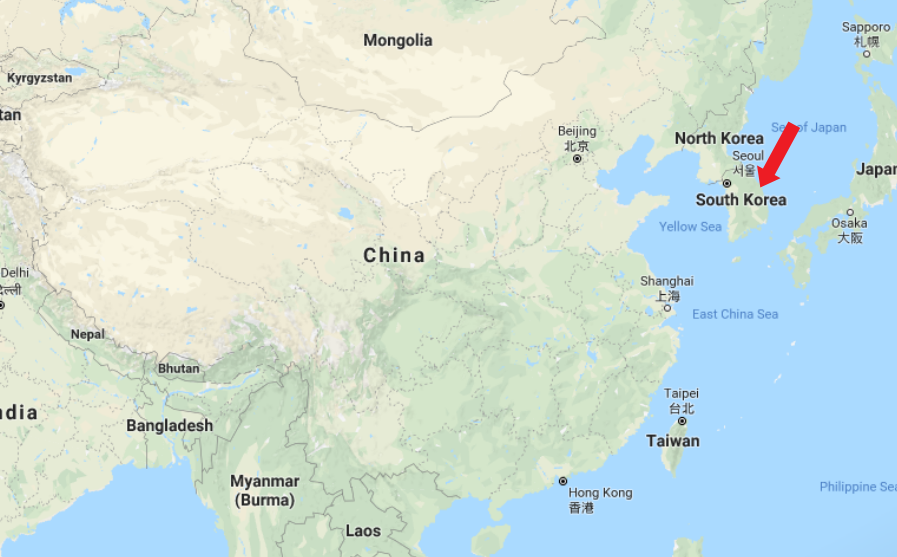
\includegraphics[width=5cm]{pictures/mymap.png}
   \begin{itemize}
    \item From South Korea (9,200 km)
      \vspace{0.3cm}
    \item Kyungpook National University, Daegu 
      \vspace{0.3cm}
    \item First year master course student in experimental high energy physics
   \end{itemize}
   \end{columns}
}

\frame{
    \frametitle{Long-lived particles (LLPs) at HL-LHC}
    \begin{itemize}
    \item No clear observation of new physics (NP) at the LHC as yet
    \vspace{0.3cm}
    \item NP portal: weakly coupled sector with long lifetime 
    \vspace{0.3cm}
    \item Long lifetimes very generic in any theory with multiple mass scales, broken symmetries... SM is a good example
    \end{itemize}
    \vspace{0.2cm}
    \begin{columns}
    \column{0.5\textwidth}
    \centering
        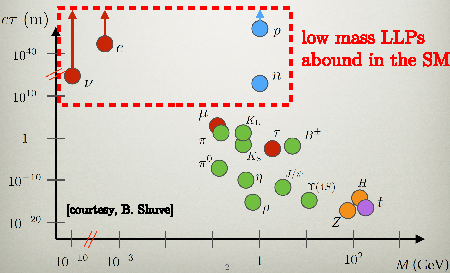
\includegraphics[width=5.5cm]{pictures/shuve_llp.pdf} \\
    \column{0.5\textwidth}
    \centering
        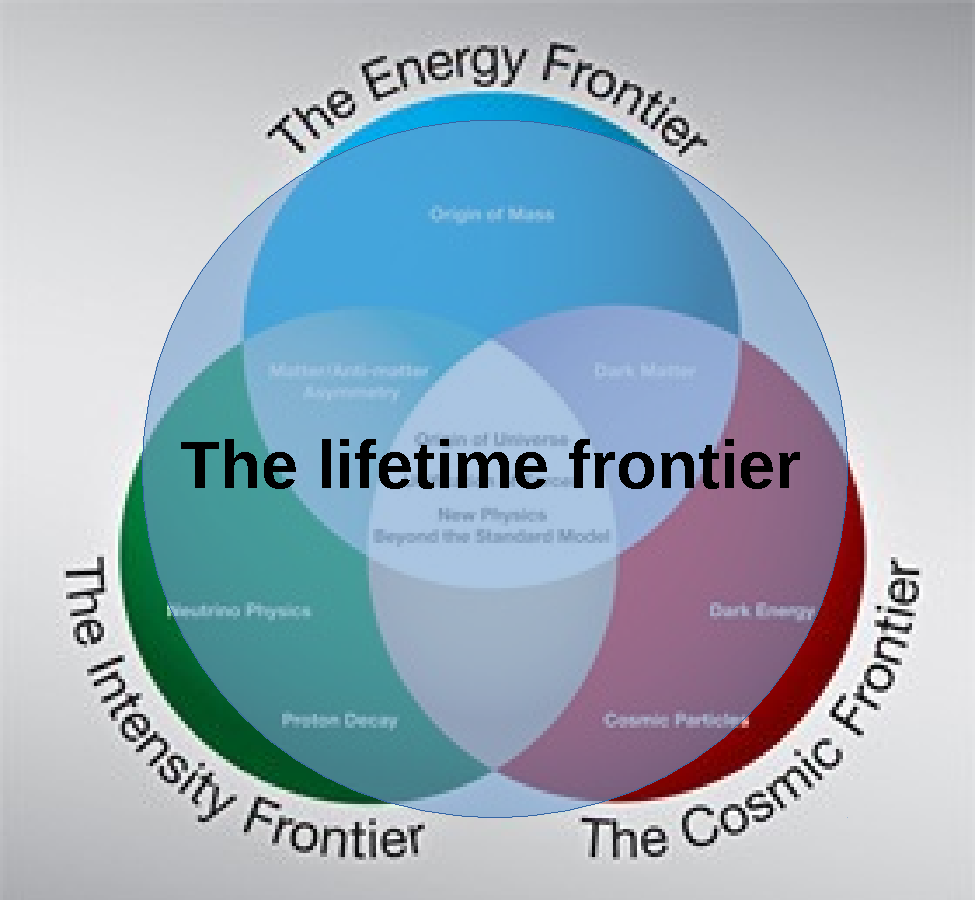
\includegraphics[width=3.8cm]{pictures/lifetime_frontier.pdf} \\
    \end{columns}
    %\item Existing detectors (ATLAS, CMS, LHCb) not optimized to find
    %\newline LLPs due to large QCD backgrounds and limited coverage
}

\frame{
    \frametitle{Other LLP detector proposals at the LHC}
   \begin{columns}
	\column{0.5\textwidth}
	\centering
    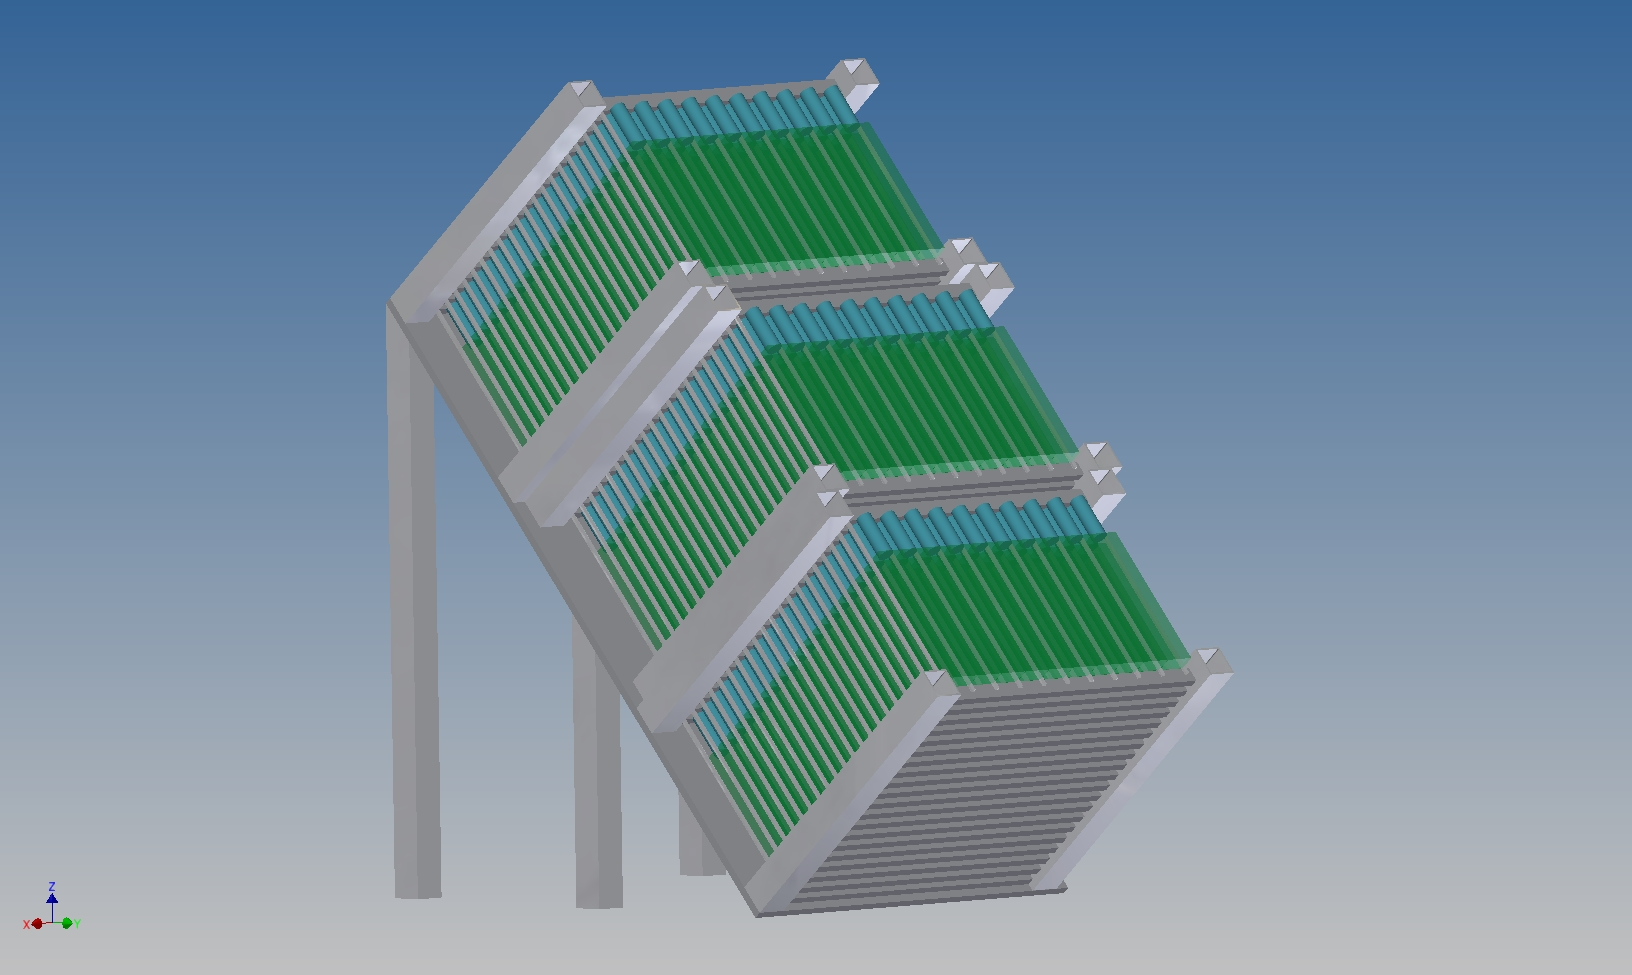
\includegraphics[width=1.9in]{pictures/milliqan}\\ {\tt MilliQan: \href{https://arxiv.org/abs/1607.04669}{\textcolor{blue}{1607.04669}}}
	\column{0.5\textwidth}
	\centering
	\vspace{-0.6cm}
	    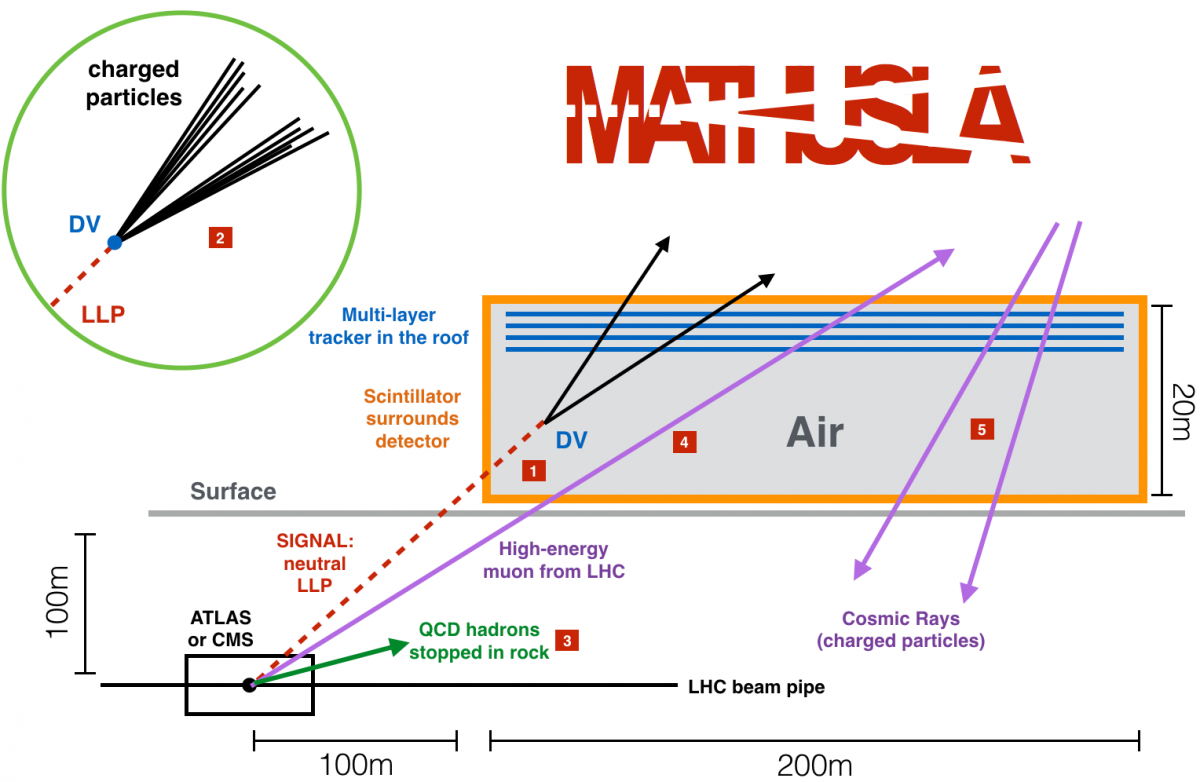
\includegraphics[width=1.9in]{pictures/mathusla}\\\vspace{0.4cm} {\tt MATHUSLA: \href{https://arxiv.org/abs/1606.06298}{\textcolor{blue}{1606.06298}}}
	\end{columns}
\vspace{0.5cm}
   \begin{columns}[T]
	\column{0.5\textwidth}
	\centering
	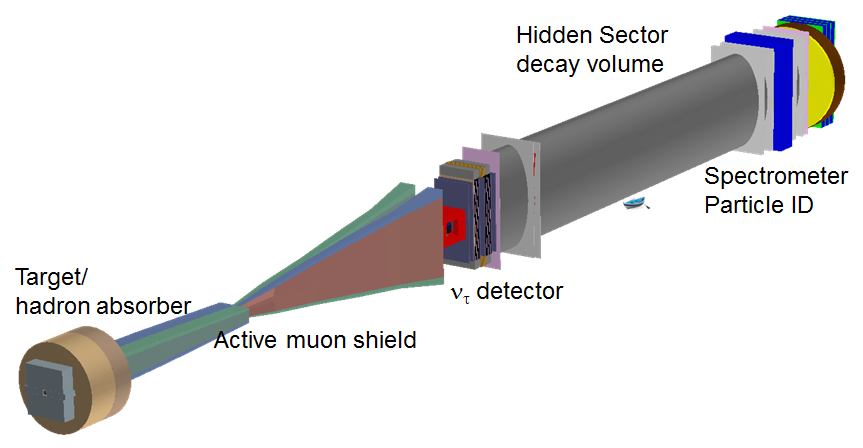
\includegraphics[width=1.78in]{pictures/ship}\\ {\tt SHiP: \href{https://arxiv.org/abs/1504.04855}{\textcolor{blue}{1504.04855}}}
	\column{0.5\textwidth}
	\centering
	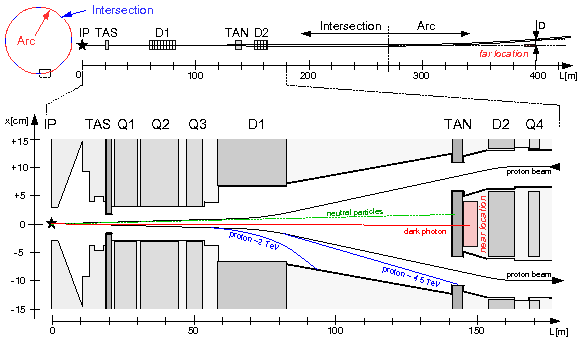
\includegraphics[width=1.6in]{pictures/faser}\\ {\tt FASER: \href{https://arxiv.org/abs/1708.09389}{\textcolor{blue}{1708.09389}}}
\end{columns}
}

\frame{
    \frametitle{Introduction - CODEX-b}
    \begin{itemize}
    \item \textbf{CO}mpact \textbf{D}etector for \textbf{EX}otics at LHC\textbf{b} (\href{https://arxiv.org/abs/1708.09395}{\textcolor{blue}{\tt 1708.09395}})
    \end{itemize}
    \vspace{0.2cm}
    \centering
    \includegraphics[width=7cm]{pictures/lhcb_cavern.pdf}
    \vspace{0.2cm}
    \begin{itemize}
    \item Move DAQ racks to surface for Run 3, instrument with tracking layers
        \vspace{0.05cm}
    \item Measure background in UXA with beam on, for physics reach studies
    \end{itemize}
}


\frame{
   \frametitle{Measurements equipment setup}
   \begin{columns}
   \column{0.5\textwidth}
   \begin{itemize}
   \item About test-bench
       \vspace{0.15cm}
   \end{itemize}
       \centering
   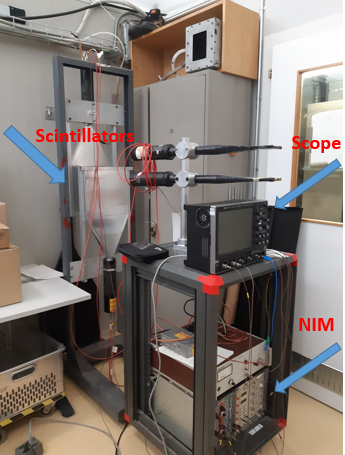
\includegraphics[width=1.9in]{pictures/Tools.png}
   \column{0.5\textwidth}
       \centering
   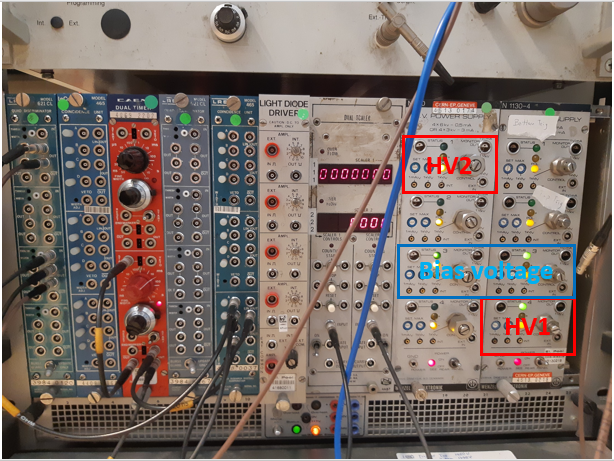
\includegraphics[width=5cm]{pictures/NIM.png}
       \vspace{0.15cm}
   \begin{itemize}
   \item Used equipments from \newline \href{https://indico.cern.ch/event/352356/contributions/1755709/attachments/697746/958057/20141202-HERSCHEL_ChallengingForUltra-HighRate.ppt}{Herschel detector}
       \vspace{0.12cm}
   \item Scintillators, PMTs, NIM, scope
   \end{itemize}
   \end{columns}
}

\frame{
   \frametitle{Scope trigger setup}
      \centering
   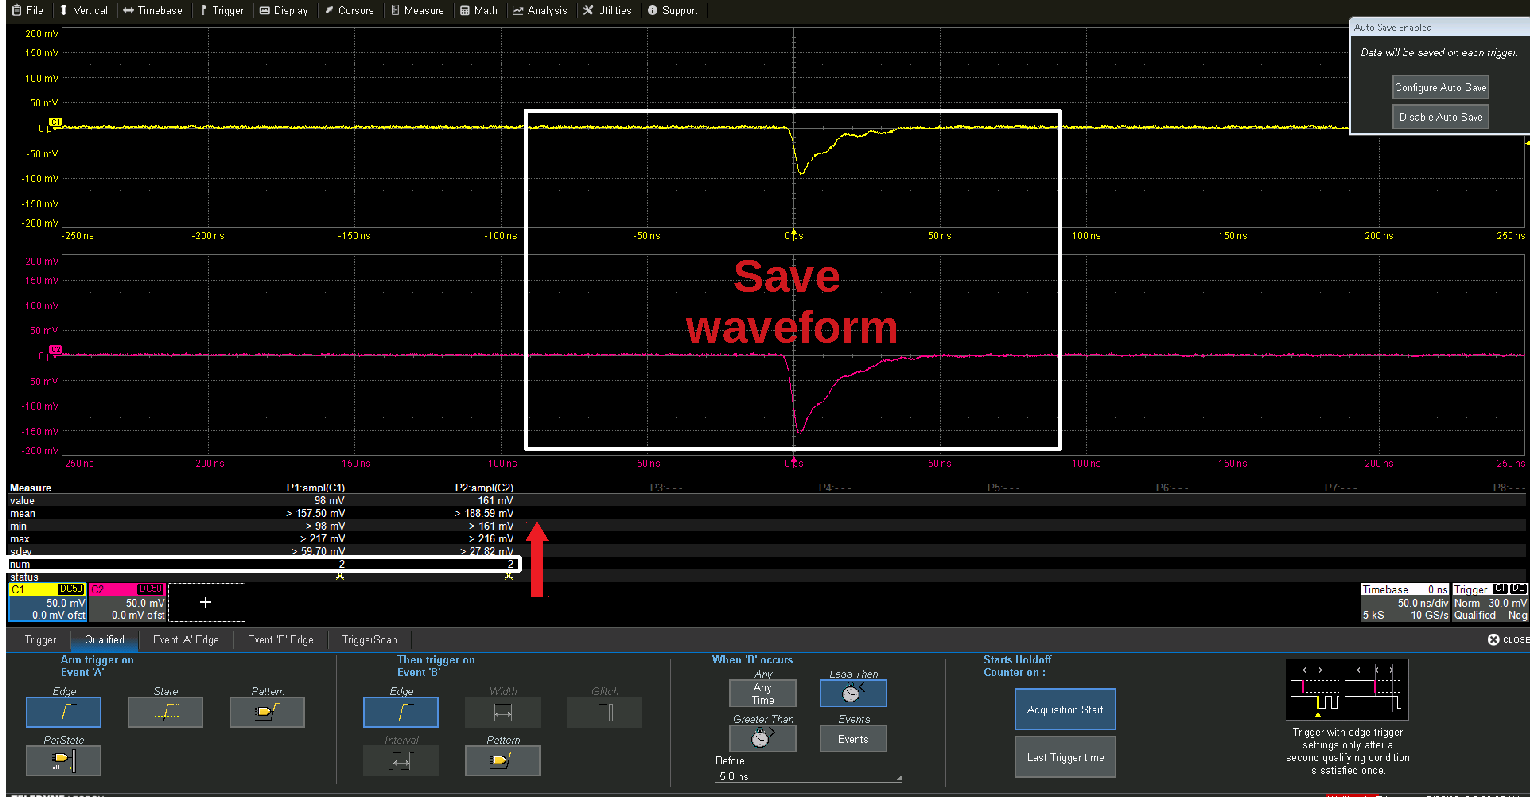
\includegraphics[width=10.5cm]{pictures/waveform.pdf}
      \vspace{0.05cm}
   \begin{itemize}
   \item Yellow - 1st scintillator (B), pink - 2nd scintillator (A)
       \vspace{0.07cm}
   \item Trigger threshold: -30 mV (falling edge)
       \vspace{0.07cm}
   \item Coincidence trigger when event A and B occur within 5 ns 
   \end{itemize}
}

\frame{
   \frametitle{Four measurement positions on D3 platform}
      \centering
   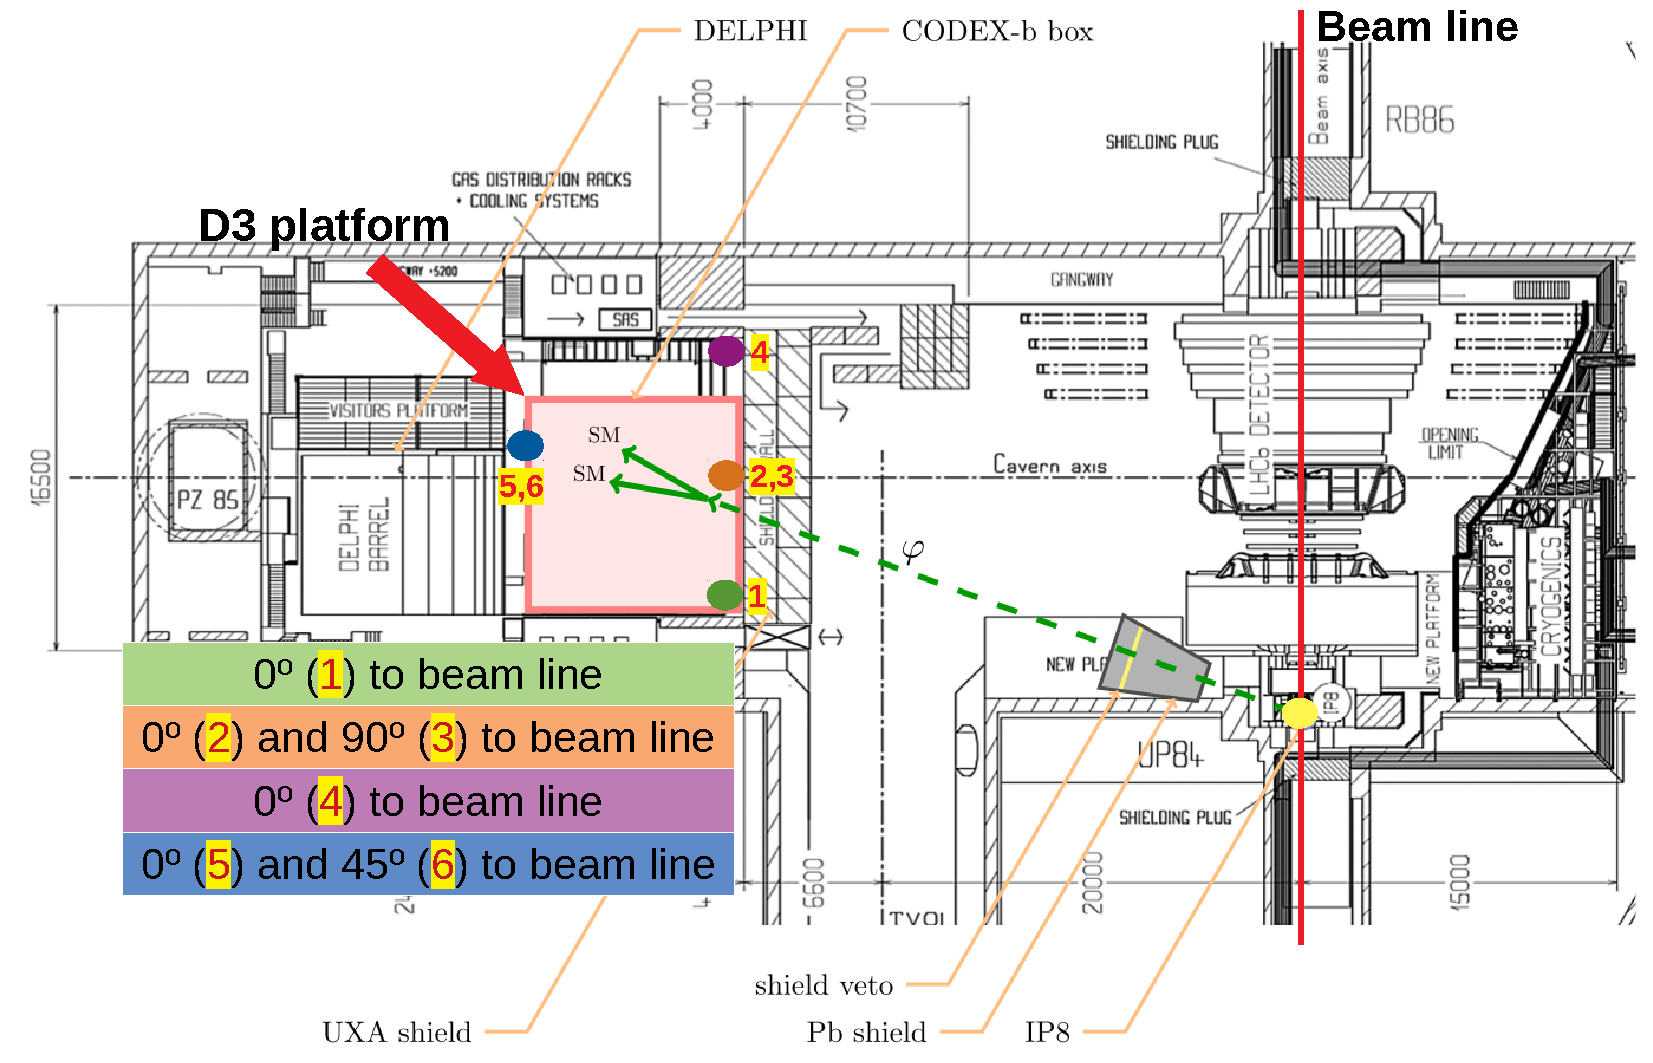
\includegraphics[width=12cm]{pictures/configuration.pdf}      
}

\frame{
   \frametitle{Measurements positions - photos}
   \begin{columns}
   \column{0.5\textwidth}
       \centering
   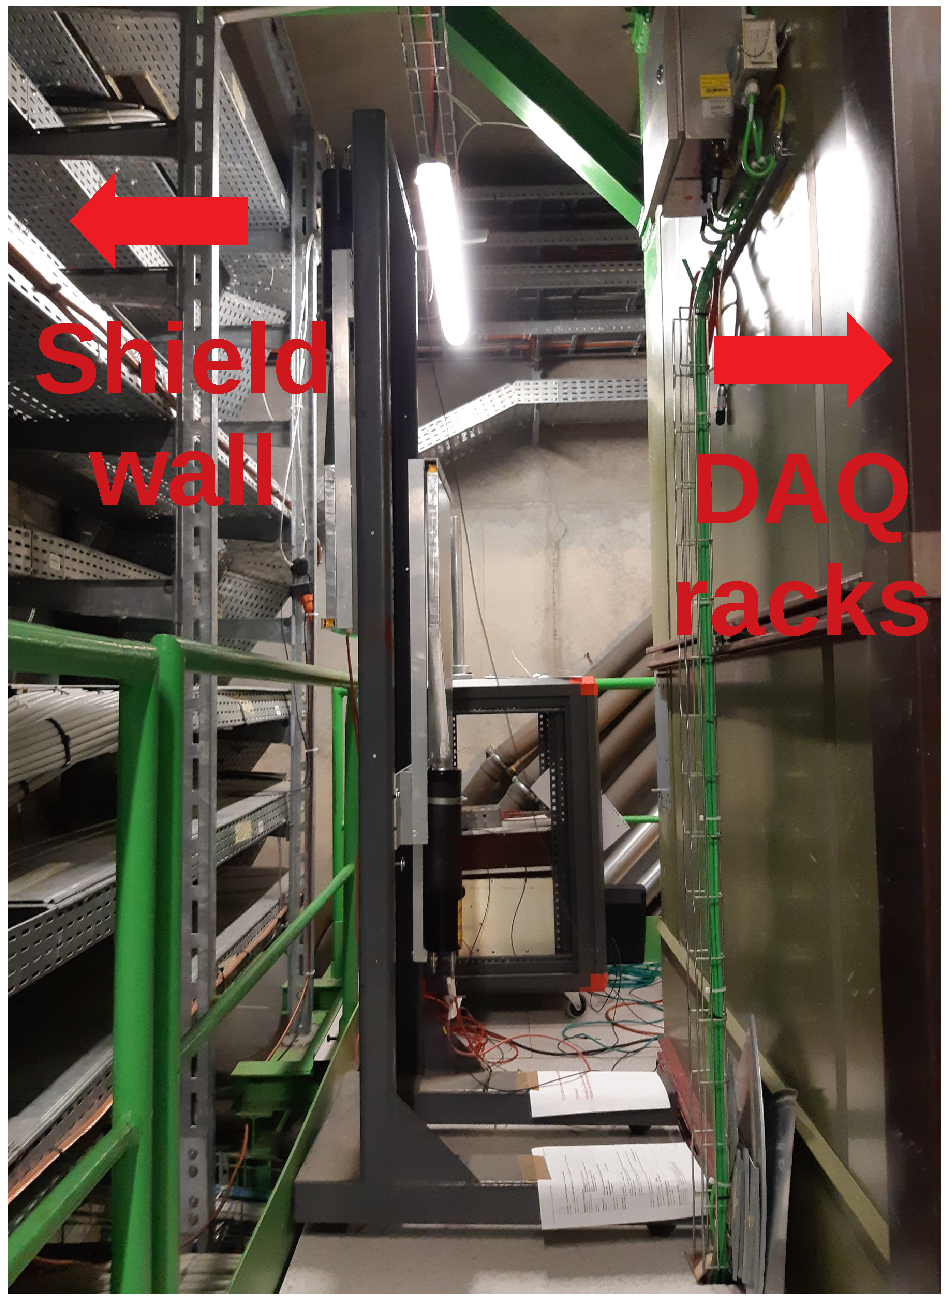
\includegraphics[width=4.5cm]{pictures/Initial.pdf}       
       \vspace{0.1cm}
   \begin{itemize}
   \item D3 back passerelle right corner
       \vspace{0.09cm}
   \item Parallel to beam line
   \end{itemize}
   \column{0.5\textwidth}
       \centering
   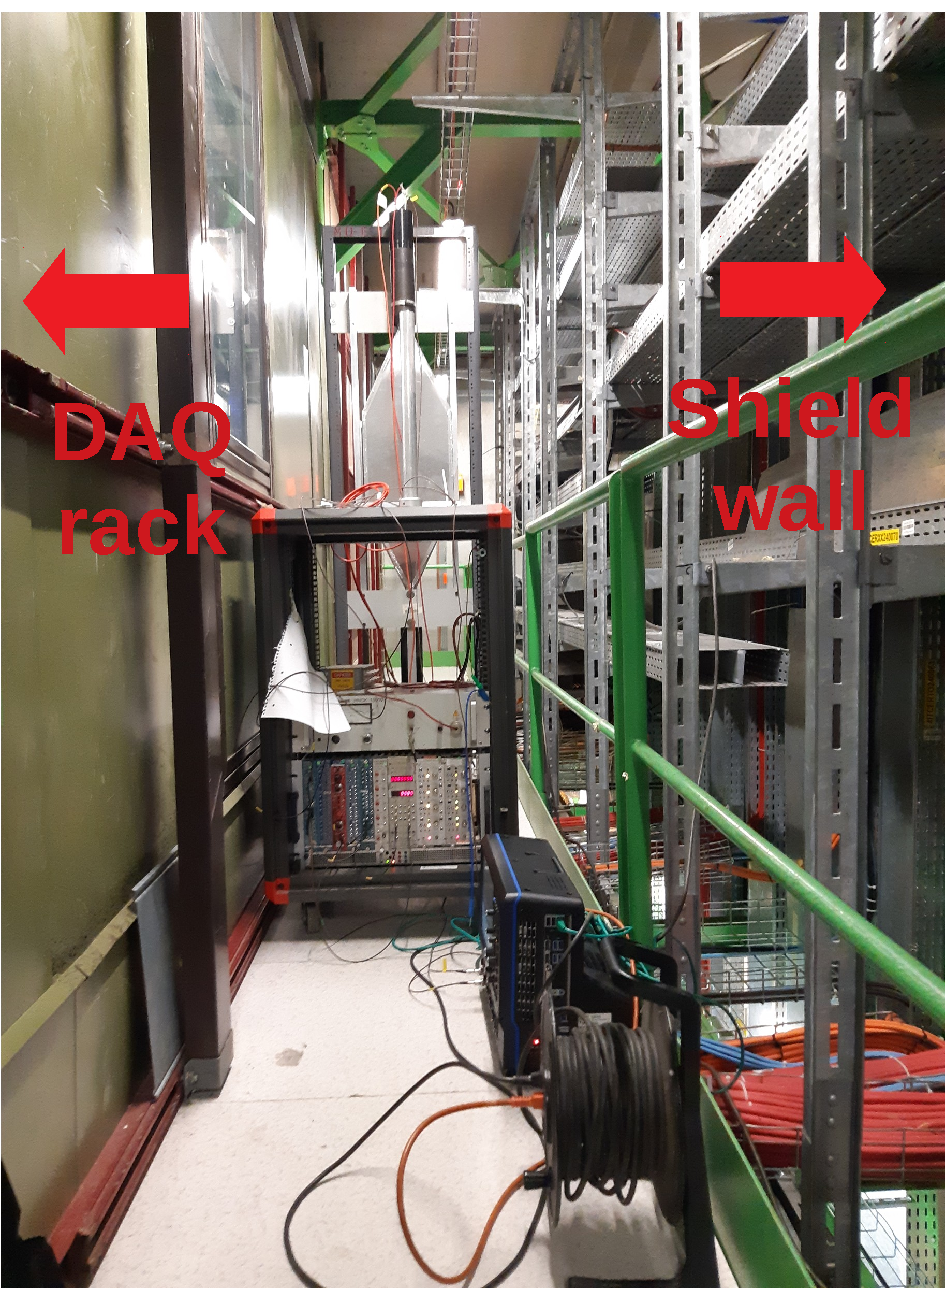
\includegraphics[width=4.5cm]{pictures/Back_central.pdf}       
       \vspace{0.1cm}
   \begin{itemize}
   \item D3 back passerelle central
       \vspace{0.09cm}
   \item Perpendicular to beam line
   \end{itemize}
   \end{columns}
}

\frame{
   \frametitle{Measurements positions - photos}
   \begin{columns}
   \column{0.5\textwidth}
       \centering
   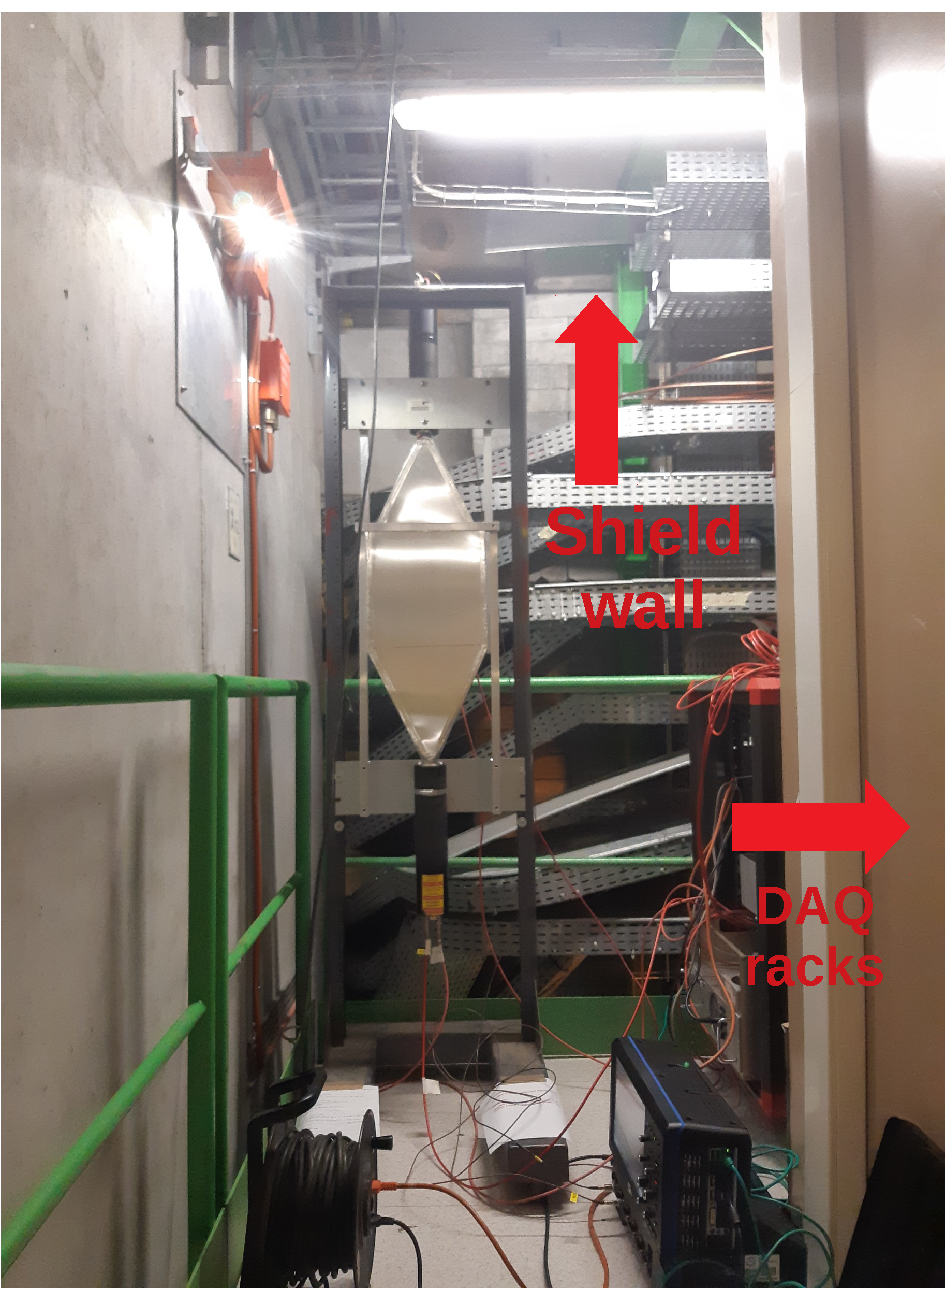
\includegraphics[width=4.5cm]{pictures/Othercorner.pdf}        
       \vspace{0.1cm}
   \begin{itemize}
   \item D3 back passerelle left corner
       \vspace{0.09cm}
   \item Parallel to beam line
   \end{itemize}
   \column{0.5\textwidth}
       \centering
   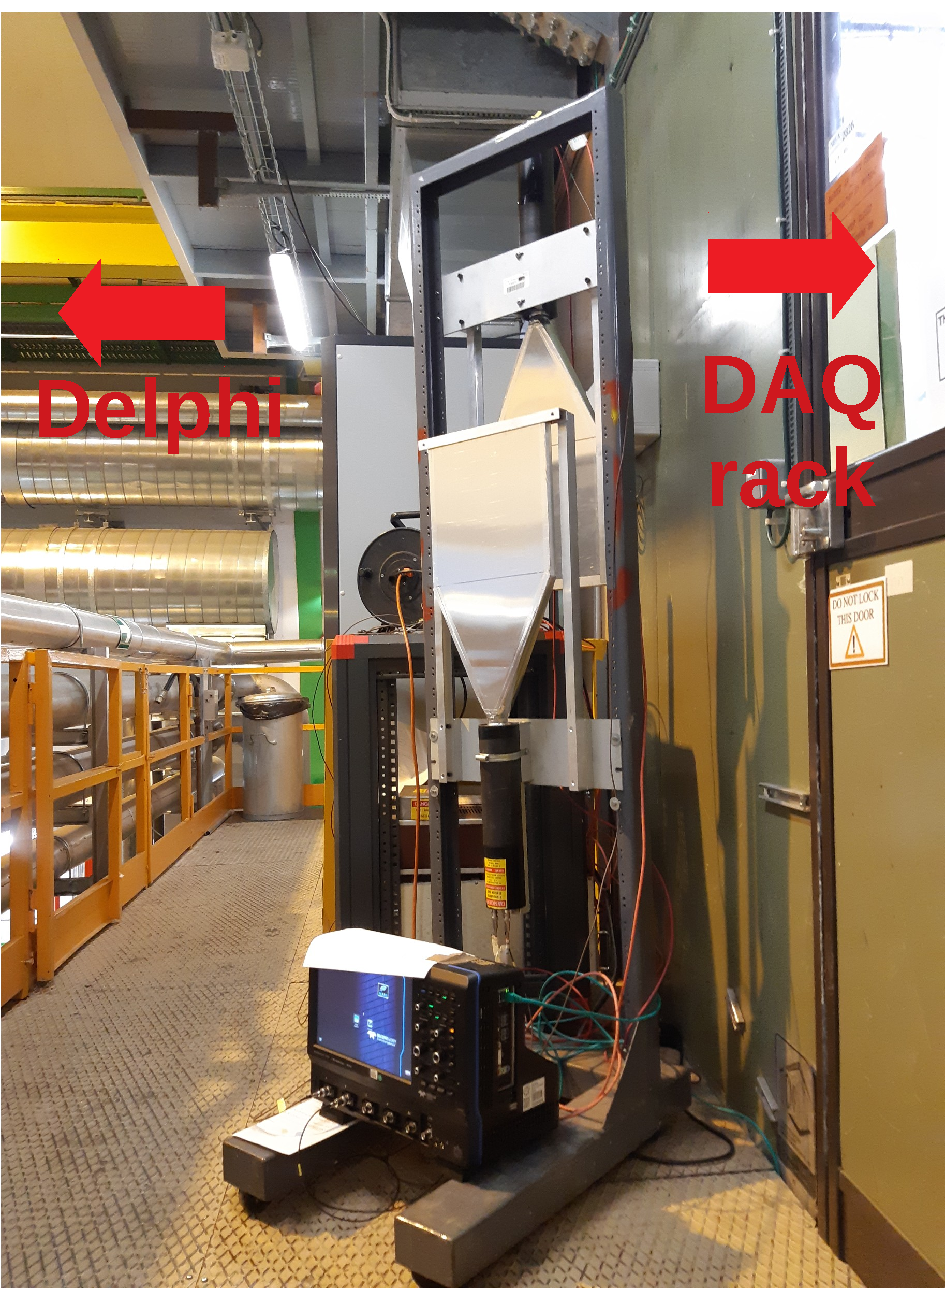
\includegraphics[width=4.5cm]{pictures/D3_front.pdf} 
       \vspace{0.1cm}
   \begin{itemize}
   \item D3 front central
       \vspace{0.09cm}
   \item 45$^\circ$ angle to beam line
   \end{itemize}
   \end{columns}
}

\frame{
   \frametitle{Global snapshot of the data}
     \vspace{-0.05cm}
     \begin{itemize}
       \item Measurement campaign spanning \textcolor{red}{17 days} in July-Aug. \textcolor{red}{52036} triggers.
       \item \textcolor{red}{6 positions/configurations} on D3 marked in blue and green, alternatingly:
     \end{itemize}
       \vspace{0.2cm}
      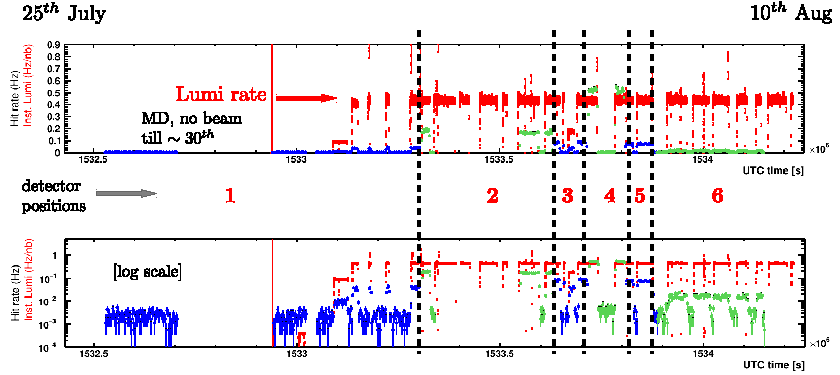
\includegraphics[width=12.4cm]{pictures/codexb_data_global.pdf}
}

\frame{
   \frametitle{Detailed features -- background rate w/o beam}
     \begin{itemize}
       \item Reminder: rate of \textcolor{blue}{$pp$} collisions + interactions is \textcolor{blue}{25~MHz} (PU=1).
       \item \textcolor{red}{Ambient} background hit rate between fills or in MD, \textcolor{red}{without beam}.
     \end{itemize}
       \vspace{0.2cm}
\begin{center}
\begin{tabular}{c|l|r}
  Position & \hspace{2cm}Description & Hit rate [mHz] \\
  \hline \hline
   P1 & shield, right corner, $\parallel$ to beam& $1.99\pm0.07$ \\ \hline
   P2 & shield, center, $\parallel$ to beam&  $2.76\pm 0.03$ \\ \hline
   P3 & shield, center, $\perp$ to beam& $ 2.26\pm 0.03$ \\ \hline
   P4 & shield, left corner, $\parallel$ to beam& $ 3.11\pm 0.03$ \\ \hline
   P5 & shield + D3 racks, center, $\parallel$ to beam& $ 1.95\pm 0.03$ \\ \hline
   P6 & shield + D3 racks, center, $45^\circ$ to beam& $ 2.22\pm $ 0.02\\ \hline
\end{tabular}
\end{center}
     \begin{itemize}
       \item Pretty consistent, \textcolor{red}{$\sim2$~mHz}, across all positions and essentially \textcolor{red}{negligible}
     \end{itemize}
}



\frame{
   \frametitle{Specific features -- rate during stable beam}
     \begin{itemize}
       \item Background hit rate during \textcolor{red}{stable beam}.
     \end{itemize}
       \vspace{0.2cm}
\begin{center}
\begin{tabular}{c|l|r}
  Position & \hspace{0.9cm}Description & Hit rate [mHz] \\
  \hline \hline
   P1 & shield, right corner, $\parallel$ to beam & $ 38.99 \pm 0.99 $\\ \hline
   P2 & shield, center, $\parallel$ to beam& $ 167.10 \pm 1.43$ \\ \hline
   P3 & shield, center, $\perp$ to beam& $ 82.81 \pm 1.55 $ \\ \hline
   P4 & shield, left corner, $\parallel$ to beam& $ 517.45 \pm 3.52 $ \\ \hline
   P5 & shield + D3 racks, center, $\parallel$ to beam& $ 73.58 \pm 1.18 $ \\ \hline
   P6 & shield + D3 racks, center, $45^\circ$ to beam& $ 15.71 \pm 0.33 $ \\ \hline
\end{tabular}
\end{center}
     \begin{itemize}
       \item Maximal rate at P4, $\sim 0.5$~Hz during beam. Calibrate simulation.
       \item The D3 racks definitely add some shielding as well (hard to simulate). 
     \end{itemize}
}

\frame{
   \frametitle{Simulation - DD4hep}
   \begin{columns}
   \column{0.5\textwidth}
   \centering
   
\includegraphics[width=5.5cm]{pictures/DD4hepLogo.png} \\
   \href{https://dd4hep.web.cern.ch/dd4hep/}{\scriptsize {\tt https://dd4hep.web.cern.ch/dd4hep/}}
   \column{0.5\textwidth}
   \begin{itemize}
   \item DD4hep is a software framework for HL-LHC upgrade 
       \vspace{0.15cm}
   \item Since CODEX-b is a new detector for HL-LHC, we chose to use it 
   \end{itemize}
   \end{columns}
   \vspace{0.35cm}
   \begin{itemize}
   \item Built CODEX-b geometry in DD4hep
       \begin{itemize}
       \item Made \textcolor{red}{hierachy system} (envelope $\rightarrow$ super station $\rightarrow$ station $\rightarrow$ layer)
           \vspace{0.1cm}
       \item Tested with a $\mu$ particle gun
           \vspace{0.1cm}
       \item Checked \textcolor{red}{energy deposits and positions} of CODEX-b hits
       \end{itemize}
   \vspace{0.2cm}
   \item Tested with \textcolor{red}{MinBias} (standalone Gauss) $\to$ HepMC format $\to$ DDG4
   \item Hits read out using DD4hep plugin, checked that they look reasonable
   \end{itemize}
}

\frame{
   \frametitle{Detector geometry in DD4hep}
   \begin{columns}
   \column{0.5\textwidth}
   \centering
       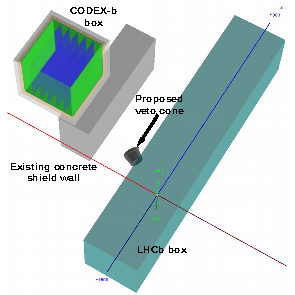
\includegraphics[width=6.5cm]{pictures/CODEXbBigGeo.pdf}
   \column{0.5\textwidth}
   \begin{itemize}
   \item Veto cone
       \vspace{0.15cm}
       \begin{itemize}
       \item {\footnotesize Two Pb absorbers}
       \vspace{0.1cm}
       \item {\footnotesize One active Si shield layer}
       \end{itemize}
   \vspace{0.2cm}
   \item Concrete shield wall
       \vspace{0.15cm}
       \begin{itemize}
       \item {\footnotesize 3.2 m thickness}
       \vspace{0.1cm}
       \item {\footnotesize Block most particles from 
       \newline \textit{pp} collisions}
       \end{itemize}
   \vspace{0.2cm}
   \item CODEX-b box
       \vspace{0.15cm}
       \begin{itemize}
       \item {\footnotesize Consists of two types of stations}
       \end{itemize}
   \end{itemize}
   \end{columns}
}

\frame{
   \frametitle{Detector geometry in DD4hep - Zoom}
   \begin{itemize}
   \item Geometry was taken from \href{https://arxiv.org/abs/1708.09395}{\textcolor{blue}{\tt 1708.09395}} (not final!)
   \end{itemize}
   \begin{columns}
   \column{0.5\textwidth}
   \centering
       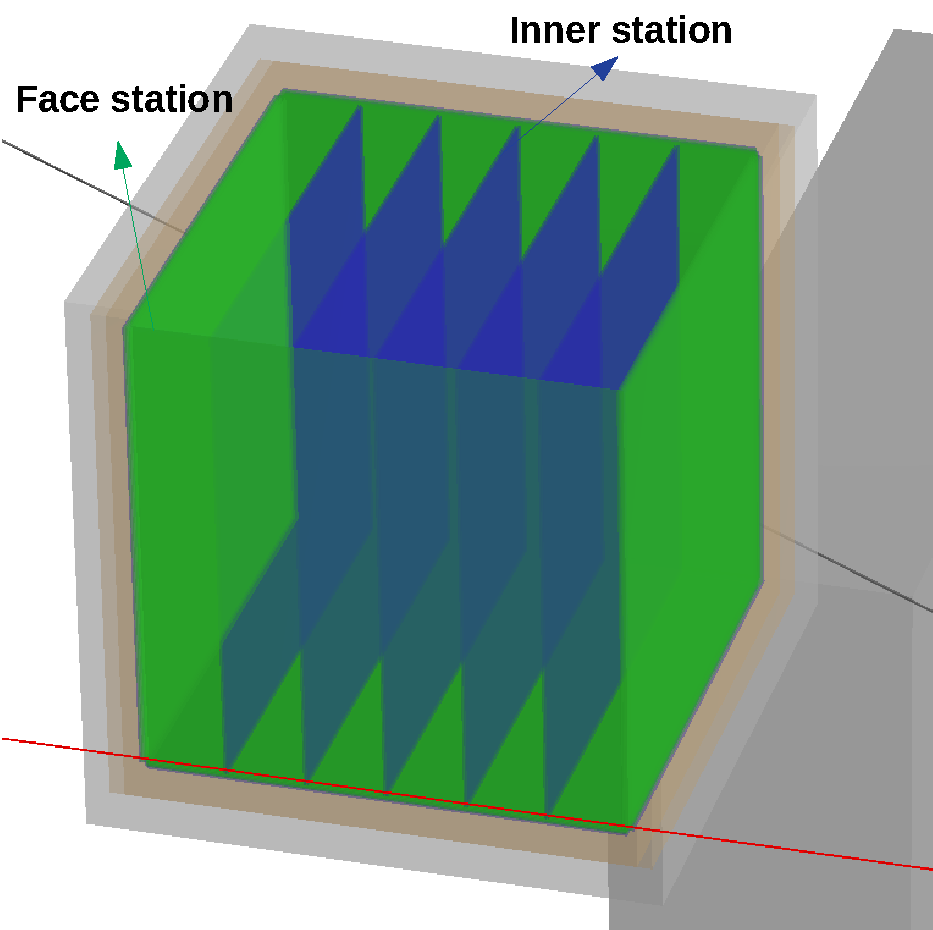
\includegraphics[width=6.2cm]{pictures/ZoomVersion.pdf}
   \column{0.5\textwidth}
   \begin{itemize}
   \item Inner station (x5)
       \vspace{0.15cm}
       \begin{itemize}
       \item {\footnotesize Silicon tracker}
       \vspace{0.1cm}
       \item {\footnotesize 3 layers of 10 x 10 $m^{2}$ size 
       \newline and 2 cm thickness}
       \vspace{0.1cm}
       \item {\footnotesize Distance between layers is 4 cm}
       \end{itemize}
   \vspace{0.2cm}
   \item Face station (x6)
       \vspace{0.15cm}
       \begin{itemize}
       \item {\footnotesize Silicon tracker}
       \vspace{0.1cm}
       \item {\footnotesize 6 layers of 10  x 10 $m^{2}$ size 
       \newline and 2 cm thickness}
       \vspace{0.1cm}
       \item {\footnotesize Distance between layers is 4 cm}
       \end{itemize}
   \end{itemize}
   \end{columns}
}

\frame{
   \frametitle{DD4hep simulation with minbias events - CODEX-b}
   \begin{itemize}
   \item 13\tev minbias events with \textcolor{red}{existing shield \textbf{removed}} 
   \end{itemize}
   \vspace{0.2cm}
   \centering
       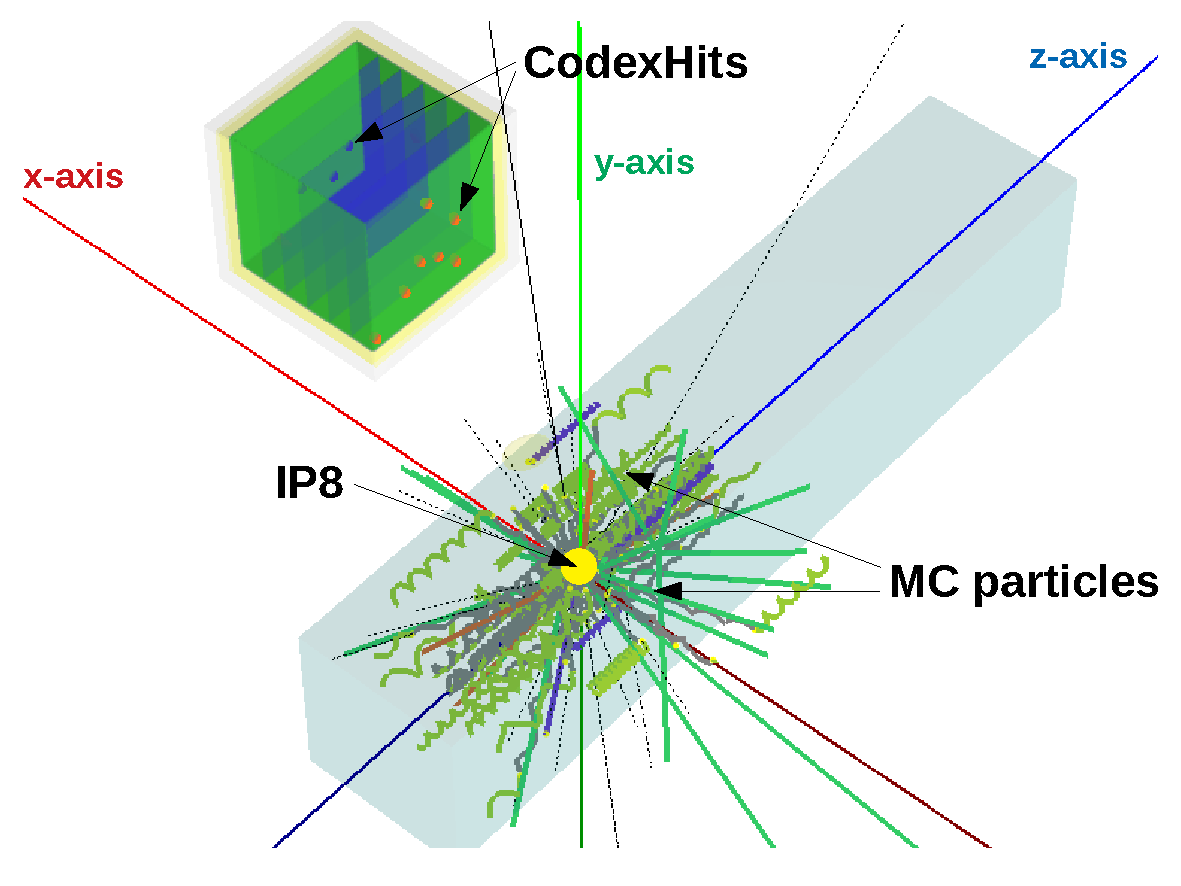
\includegraphics[width=9cm]{pictures/Minbias.pdf}
}

\frame{
   \frametitle{DD4hep simulation with minbias events - scintillators}
   \vspace{-0.2cm}
   \begin{itemize}
   \item \textcolor{red}{32k events}, generated in \textcolor{red}{4$\pi$}, using {\tt minbias.dec}, \textcolor{red}{no hits!}
   \end{itemize}
   \centering
       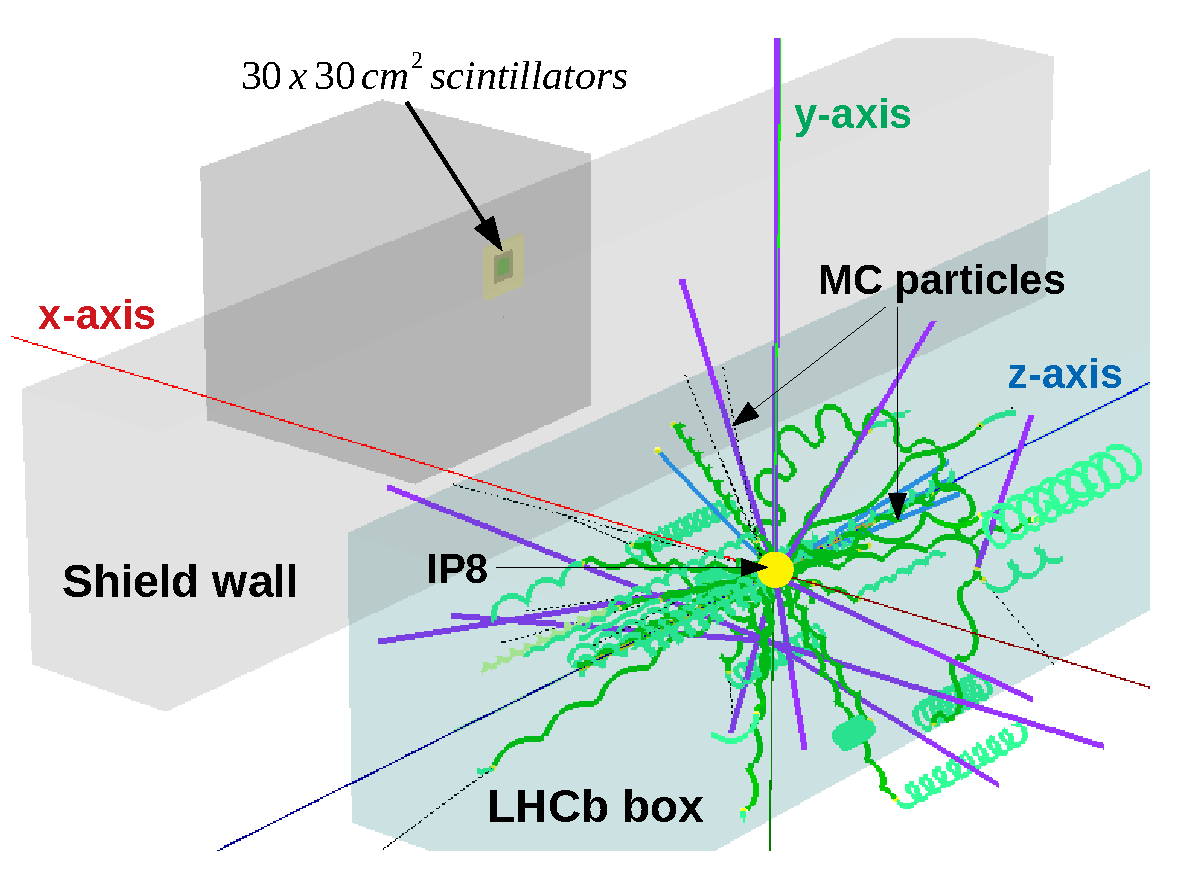
\includegraphics[width=8.5cm]{pictures/Scint.pdf}
   \vspace{0.05cm}
   \begin{itemize}
   \item New dec file with generator cuts is work in progress
   \end{itemize}

}

\frame{
   \frametitle{Summary and future plan}
   \begin{itemize}
   \item Very \textcolor{red}{successful} background measurement \textcolor{red}{campaign} at D3
       \vspace{0.42cm}
   \item Background \textcolor{red}{rate} just behind shield wall around \textcolor{red}{0.5~Hz} over \textcolor{red}{900cm$^{2}$}
       \vspace{0.42cm}
   \item \textcolor{red}{DD4hep-based} \textcolor{red}{simulation} fully tested both measurement and CODEX-b configurations
       \vspace{0.42cm}
   \item Working on more efficient MC generation in Gauss \textcolor{red}{w/ generator cuts}
       \vspace{0.42cm}
   \item {Presented at \href{https://indico.cern.ch/event/722726/contributions/3102422/attachments/1699623/2736731/talk8.pdf}{\textcolor{blue}{Run meeting}} on 10/08}
       \vspace{0.42cm}
   \item Once simulation is ready, finalize the \textcolor{red}{internal note}
   \end{itemize}
}

\frame{
   \frametitle{Acknowledgements}
   \begin{itemize}
   \item My summer student supervisors: Biplab Dey, Victor Coco
       \vspace{0.2cm}
   \item DD4hep developer: Markus Frank
       \vspace{0.2cm}
   \item Equipments from Herschel detector: Heinrich Schindler, Raphael Dumps
       \vspace{0.2cm}
   \item Theoretical parts: Vladimir Gligorov
       \vspace{0.2cm}
   \item At the pit: Tengiz Kvaratskheliya
   \end{itemize}
   \vspace{0.3cm}
   \pause
       \centering
       {\Large Thanks to LHCb for a wonderful experience !}
}

\frame{
    \centering
    {\Huge \textbf{Thank you}}
}


%\section{Event Selection and $S/B$ Separation}


%\frame{
%   \vspace{2cm}
%   \centering
%\framebox{\parbox{\dimexpr\linewidth-2\fboxsep-2\fboxrule}{
%   {\Large Note: All results are very preliminary, and do not represent official $\babar$ results}}}
%
%}


\frame{
  \frametitle{Semi-leptonic $B$ decays}
       \vspace{-0.2cm}
      \begin{itemize}
          \item \textcolor{red}{Cleanest} source of \textcolor{red}{$\BB$ pairs} for studying SL $B$ decays: \\ \vspace{0.05cm} \hspace{1.5cm}$\textcolor{red}{e^+ e^-} \to \ups \overset{{\Tiny \textcolor{red}{> 96\%}}}{\to} \textcolor{red}{\BB}$, $\sqrts = \textcolor{red}{10.58}$~GeV
          \vspace{0.15cm}
          \item PEP-II collider and \textcolor{red}{$\babar$} detector: asymmetric $e^+ e^-$ $B$-factory at SLAC. %Data-taking between 1999-2008, but analyses ongoing. 
          %\item \textcolor{red}{$\babar$}: multipurpose detector for PEP-II $e^+ e^-$ asymmetric storage ring at SLAC. 
      \end{itemize}
\vspace{0.05cm}
  \begin{columns}
    \column{0.55\textwidth}
      \begin{itemize}
          \item \textcolor{red}{Full} ``on-peak'' $\babar$ dataset: \textcolor{red}{$\sim 470$~M $\BB$} pairs
          \vspace{0.3cm} 
           \item Looking at $\Bbar \to \textcolor{red}{X_{\{c,u\}}} \ell^- \barnuell$, $\textcolor{red}{X_{\{c,u\}}} \in \{\textcolor{red}{D, D^\ast, \rho} \}$
          \vspace{0.3cm} 
          \item \textcolor{red}{Tagged} analysis w/ setup similar to recent $\Bbar \to D^{(\ast)} \tau^- \bar{\nu}_\tau$ analysis ({\small PRL 109, 101802 (2012)}).
      \end{itemize}

    \column{0.45\textwidth}
       \vspace{-0.3cm}
       \centering
       { \textcolor{red}{$B^- \to \rhoz(\to \pip \pim) \mu^- \nu_{\mbox{\tiny miss}}$}}:\\ \vspace{0.3cm}
       \includegraphics[width=2in]{figs/data_anal/dpf13_babar_rho0lnu_event.jpg}
  \end{columns}
}




\frame{
   \frametitle{The BReco technique at $B$-factories}% and untagged/tagged measurments}
   \vspace{-0.1cm}
         \begin{itemize}
            \item In $e^+ e^- \to \FourS \to \bsig\btag$, \textcolor{red}{full hadronic reconstruction} of $\btag$ (\textcolor{red}{BReco}) in $\sim 3000$ modes. 
         \end{itemize}
   \begin{columns}
      \column{0.5\textwidth}
         \vspace{-0.1cm}
         \begin{itemize}
            %\item In $e^+ e^- \to \FourS \to \bsig\btag$, \textcolor{red}{full hadronic reconstruction} of $\btag$ (\textcolor{red}{BReco}) in $\sim 3000$ modes
            \item \textcolor{blue}{$\btag\to$} \textcolor{DarkGreen}{$Y_{\scriptsize \text{had}}$ ($\pi$'s and $K$'s)} + \textcolor{DeepPink}{charm ``Seed''}.
            \vspace{0.2cm}
            \item A \textcolor{red}{single missing $\nu$}: reconstructed as $p_{\scriptsize \text{miss}}$ via kinematic fit. 
            %\item Similar to $e^+ e^- \to \psi(3770) \to \dtag \dsig$ in CLEO-c/BESIII
            %\vspace{0.5cm}
            %\item Can't go to $\bsig$ RF w/o BReco
         \end{itemize}
      \column{0.55\textwidth}
         %\centering
         \includegraphics[width=2.6in]{figs/intro/breco.pdf}
   \end{columns}
   \vspace{0.3cm} 

   \begin{itemize}
       \item \textcolor{blue}{Untagged} analyses: can't go to $\bsig$ RF; \textcolor{blue}{can't measure $\{\qsq, \ctl, \ctv, \chi\}$} directly.
       %\vspace{0.3cm} 
       %\item Similar techniques at \textcolor{red}{charm}-factories \textcolor{red}{$e^+ e^- \to \psi(3770) \to \dsig \dtag$}.  
   \end{itemize}
}



\frame{
   \frametitle{The BReco technique at $B$-factories (cntd.)}% and untagged/tagged measurments}
   \begin{columns}
      \column{0.5\textwidth}
         \centering
         \includegraphics[width=2.4in]{figs/intro/rho0_resolution_poster.pdf} \\ {\em Percent} level \textcolor{red}{resolution} due to BReco
      \column{0.5\textwidth}
         \begin{itemize}
            \item Very \textcolor{red}{clean} $\bsig$ sample. 
            \vspace{0.5cm}
            \item \textcolor{red}{Fantastic resolution} in reconstruction of angular variables  
         \end{itemize}
   \end{columns}

    \vspace{0.6cm}

    \begin{itemize}
        \item Gives $B$-factories an advantage over LHCb for neutrinos.
    \end{itemize}
}



%\frame{
%   \frametitle{The BReco technique at $B$-factories (cntd.)}% and untagged/tagged measurments}
%   \vspace{-0.1cm}
%   \begin{columns}
%      \column{0.6\textwidth}
%         \vspace{-0.1cm}
%         \begin{itemize}
%            \item In $e^+ e^- \to \FourS \to \bsig\btag$, \textcolor{red}{full hadronic reconstruction} of $\btag$ (\textcolor{red}{BReco}) in $\sim 3000$ modes
%            \vspace{0.2cm}
%            \item A \textcolor{red}{single missing $\nu$} and BReco together allows direct \textcolor{red}{access} to all \textcolor{red}{final state momenta}
            %\item Similar to $e^+ e^- \to \psi(3770) \to \dtag \dsig$ in CLEO-c/BESIII
            %\vspace{0.5cm}
            %\item Can't go to $\bsig$ RF w/o BReco
%         \end{itemize}
%      \column{0.55\textwidth}
         %\centering
%         \includegraphics[width=2in]{figs/intro/breco.pdf}
%   \end{columns}
%   \vspace{0.3cm} 
 
   %\pause
%   \begin{columns}
%      \column{0.4\textwidth}
%         \centering
%         \includegraphics[width=1.8in]{figs/intro/rho0_resolution_poster.pdf} \\ {\scriptsize {\em Percent} level \textcolor{red}{resolution} due to BReco}
%      \column{0.6\textwidth}
%         \begin{itemize}
%            \item Very \textcolor{red}{clean} $\bsig$ sample, with \textcolor{red}{fantastic resolution} in reconstruction of angular variables  
%            \vspace{0.1cm}
%            \item Gives $B$-factories a distinct advantage over LHCb for neutrinos.
            %\item \textcolor{blue}{Untagged} $\Rightarrow$ \textcolor{blue}{no access} to \textcolor{blue}{$\bsig$ RF}. Kinematic variables not measured!
            %\pause
            %\item Note: angular analysis/motivations quite similar to $\Bbar_d \to \overline{K^\ast} \ell^- \ell^+$, except SM contribution is large now and we ``detect'' both leptons indirectly using BReco.
            %\vspace{0.3cm}
            %\item Technique meant for signal-side neutrino(s). Optimal for a {\em single} missing neutrino.
            %\item Low efficiency ($\sim \mathcal{O}(0.1\%)$), but expected to become the de facto method at Belle~II. 
            %\vspace{0.3cm}
            %\item {\em BReco not possible at a hadronic collider}. LHCb can do $B\to V\ell^-\ell^+$, but $\Bbar \to V \ell^- \barnuell$ is difficult. 

%         \end{itemize}
%   \end{columns}
%}





\frame{
   \frametitle{Event Selection} 


     \begin{itemize}
        \item $\FourS \to \textcolor{red}{\btag X_{\{c,u\}} \ell} \;(\nu_{\scriptsize \text{miss}})$ \textcolor{red}{fully reconstructed}. No extra charged tracks. Flavor and charge constraints automatically satisfied. 
        \vspace{0.3cm}
          \item Two \textcolor{blue}{tag-side} discriminating variables:
      \end{itemize}
         \vspace{-0.1cm}
      \begin{align}
         \textcolor{blue}{\de} &= E_{\mbox{{\scriptsize tag}}} - E_{\mbox{{\scriptsize beam}}} \;(\sim \textcolor{blue}{0} \; \text{for signal}) \nonumber \\ 
         \textcolor{blue}{\mes} &=\sqrt{E^2_{\mbox{{\scriptsize beam}}} - |\vec{p}_{\mbox{{\scriptsize tag}}}|^2} \;(\sim \textcolor{blue}{m_B} \; \text{for signal})\nonumber
         %\textcolor{blue}{\de} &= E^\ast_B - \sqrts/2 \;(\sim \textcolor{blue}{0} \; \text{for signal}) \nonumber \\ 
         %\textcolor{blue}{\mes} &=\sqrt{s/4 - |\vec{p}^\ast_B|^2} \;(\sim \textcolor{blue}{m_B} \; \text{for signal})\nonumber
       \end{align}
         \vspace{-0.15cm}
     \begin{itemize}
        \item Since $p_\nu \equiv p_{\scriptsize \text{miss}}$, \textcolor{red}{signal}-fit variable is:\\
        \begin{equation} 
            \textcolor{red}{U = E^\ast_\nu - |\vec{p}^\ast_\nu|}\;\;(\text{in } B\text{ RF}) \nonumber
        \end{equation} 
        \item Skim-level selection: \textcolor{blue}{$\mes > 5.27$}~GeV, \textcolor{blue}{$|\de| < 72$}~MeV and \textcolor{red}{$|U| < 0.4$}~GeV. Already a well-constrained system. 
      \end{itemize}
}

\frame{
    \frametitle{Other $S/B$ Discriminating Variables}

   \begin{columns}
      \column{0.7\textwidth}
          \normalsize
          \begin{itemize}
              \item Require \textcolor{red}{good photons} to deposit $\geq \textcolor{red}{50}$~MeV/cluster in the calorimeter
              \vspace{0.2cm}
              \item \textcolor{red}{$\eext$} is sum of energies of \textcolor{red}{extra good photons} not used in event reconstruction (bkgd. in the EMC)
          \end{itemize}
      \column{0.3\textwidth}
       \centering
       \includegraphics[width=1.4in]{figs/data_anal/zurich_talk_eex.pdf} 
   \end{columns}
   \begin{columns}
      \column{0.7\textwidth}
          \begin{itemize}
          \normalsize
              \item \textcolor{red}{$\Delta \thrustA$}: angle between $\btag$ and Rest-Of-Event \textcolor{red}{thrust axes} (direction that maximizes the longitudinal momentum) 
              \vspace{0.2cm}
              \item \textcolor{red}{$\BB$} events are \textcolor{red}{isotropic}, while \textcolor{blue}{$\qqb$} (\textcolor{blue}{continuum}) events are \textcolor{blue}{jet-like}. 
          \end{itemize}
      \column{0.3\textwidth}
       \includegraphics[width=1.4in]{figs/data_anal/zurich_talk_cosT.pdf} 
   \end{columns}
}

\frame{
   \frametitle{Kinematic Fitting}
    \begin{itemize}
      \item ``Standard'' fit (\textcolor{red}{Fit~I}):
      \vspace{0.2cm}
      \begin{itemize}
        \normalsize
         \item except for $\rho$, \textcolor{red}{$X$} is \textcolor{red}{mass-constrained}
         \vspace{0.2cm}
         \item except for $D$, \textcolor{red}{$X$} vertex is \textcolor{red}{beam-spot}-constrained
         \vspace{0.2cm}
         \item both \textcolor{red}{$\bsig$} and \textcolor{red}{$\btag$} are \textcolor{red}{mass-constrained}
         \vspace{0.2cm}
         \item the \textcolor{red}{$\ups$} candidate vertex is constrained to the \textcolor{red}{beam-spot}
         \vspace{0.2cm}
         \item The signal variable \textcolor{red}{$U$} comes from \textcolor{red}{Fit~I}
      \end{itemize}
      \vspace{0.4cm}
    \item Additional fit (\textcolor{red}{Fit~II}):
      \begin{itemize}
        \normalsize
        \vspace{0.2cm}
        \item Additionally, \textcolor{red}{$\nu$} \textcolor{red}{mass-constrained} as well
        \vspace{0.2cm}
        \item All kinematic variables \textcolor{red}{other than $U$} come from \textcolor{red}{Fit~II}.
      \end{itemize}
   \end{itemize}
}

\frame{
   \frametitle{Event selection: $\Bbar \to D^\ast \ellm \barnuell$}
    \begin{itemize}
       \item Require \textcolor{red}{$\deltam \equiv m(D^\ast) -m(D)$} less than $4\sigma$ around nominal value, where $\sigma$ is the expected resolution.
        \vspace{0.5cm}
       \item $\Bbar \to \textcolor{red}{D^\ast (\to D \pi)}\; \ellm \barnuell$ is \textcolor{red}{{\em very} clean} after this selection.
        \vspace{0.5cm}
       \item Carefully select only \textcolor{red}{six clean modes} with \textcolor{red}{$\sim 2\%$} background after CL cut from \textcolor{red}{Fit~II} (\textcolor{red}{$\nu$ mass-constrained} in Kin. Fit). 
        \vspace{0.5cm}
       \item \textcolor{red}{{\em No background-subtraction needed!}}
    \end{itemize}
}

\frame{
   \frametitle{Event selection: $\Bbar \to D^\ast \ellm \barnuell$ (cntd.)}
\vspace{-0.1cm}
    \begin{itemize} 
      \item Expected yield and $B/S$ estimates using MC, w/ $|U|<50$~MeV cut:
    \end{itemize} 
\vspace{0.1cm}

  \begin{columns}
    \column{0.5\textwidth}
     \centering
     \underline{$D^{\ast+} \to \Dz \pip$}
\vspace{0.2cm}

\begin{tabular}{l c c }
  $\Dz$ Mode & $S$ & $B/S (10^{-2})$ \\ \hline
 $K^-\pip$ & 825 & 1.1\\ \hline
 $K^-\pip \piz$ & 1434 & 1.4 \\ \hline
 $K^-\pip \pim \pip$ & 943 & 1.3\\ \hline
\end{tabular}
    \column{0.5\textwidth}
     \centering
     \underline{$D^{\ast 0} \to \Dz \piz$}
\vspace{0.2cm}

\begin{tabular}{l c c }
  $\Dz$ Mode & $S$ & $B/S (10^{-2})$ \\ \hline
 $K^-\pip$ & 873 & 2.5\\ \hline
 $K^-\pip \piz$ & 1193 & 2.6\\ \hline
 $K^-\pip \pim \pip$ & 825 & 2.6\\ \hline
\end{tabular}
  \end{columns}
 \vspace{0.3cm}
  \begin{columns}
    \column{0.5\textwidth}
    \centering
    \includegraphics[width=2.2in]{figs/data_anal/bdslnu.pdf} 
    \column{0.5\textwidth}
    \begin{itemize} 
      \item Remarkably clean dataset! 
       \vspace{0.4cm}
    \end{itemize} 
     \centering
      \fcolorbox{red}{yellow}{$\sim 6000$ events w/ $\sim 2\%$ bkgd.}
   \end{columns}
}


\frame{
   \frametitle{Event selection: $\Bbar \to D \ellm \barnuell$}

     \vspace{0.3cm}
  \begin{columns}
    \column{0.45\textwidth}

     \vspace{-0.6cm}
    \begin{itemize} 
      \item \textcolor{red}{Five} clean enough modes: 
     \vspace{0.1cm}
    \begin{itemize}
       \normalsize
        \item $\Dz \to K^-\pip$  
        \vspace{0.05cm}
        \item $\Dz \to K^- \pip \piz$
        \vspace{0.05cm}
        \item $\Dz \to K^- \pip \pim \pip $
        \vspace{0.05cm}
        \item $\Dp \to K^- \pip \pip $
        \vspace{0.05cm}
        \item $\Dp \to K^- \pip \pip \piz $
    \end{itemize}
     \vspace{0.8cm}
     \item \textcolor{red}{Loose cuts}: $\eext < 0.8$~GeV and CL from Fit~I $\geq 10^{-8}$ 
    \end{itemize} 

    \column{0.6\textwidth}
    \vspace{-1.4cm}
    \begin{itemize} 
      \item Main background: feed-down from $D^\ast$ 
    \end{itemize} 
    \begin{center}
    \includegraphics[width=2.5in]{figs/data_anal/btodlnu_stack_2.pdf} \\ \vspace{-1.4cm} \hspace{3cm} {\small {\tt [Not approved]}} 
    \end{center}

  \end{columns}

      \vspace{0.2cm}
    \begin{itemize} 
      \item Note the \textcolor{red}{smooth} nature of the \textcolor{red}{background shape} under the signal  
      \vspace{0.2cm}
      \item Caveat: ``out-of-the-box'' existing generic $\babar$ MC. MC {\em not} fitted to Data.
    \end{itemize} 
}

\frame{
   \frametitle{Event selection: $\Bbar \to \rhoz \ellm \barnuell$}
    \begin{itemize} 
      \item For \textcolor{red}{charmless} modes ($\{\pi, \rho,\omega,...\}$), the \textcolor{red}{$e/\mu$} samples have to be processed \textcolor{red}{separately}
      \vspace{0.45cm}
      \item \textcolor{red}{$\pi \leftrightarrow \mu$ misId}: bkgd. characteristics very different between $e/\mu$ 
      \vspace{0.45cm}
      \item \textcolor{red}{$\mu$} sample has more $\qqb$ \textcolor{red}{continuum} bkgd. that hadronizes to multi-charmless final states and \textcolor{red}{nothing missing. $|\vec{p}_{\text{\scriptsize miss}}| > 0.3$} GeV.
      \vspace{0.45cm}
      \item Tighter \textcolor{red}{$|\cosT|$} cuts for \textcolor{red}{$\mu$} sample for \textcolor{red}{continuum suppression}.
      \vspace{0.45cm}
      \item \textcolor{red}{$e$ signal} shape has a long \textcolor{red}{tail} at high $U$ due to larger \textcolor{red}{brem.} 
      \vspace{0.45cm}
      \item \textcolor{red}{$M(\pi \pi) \in[0.67,0.87]$}~GeV. {\em Assume} no $S$-wave (checks done using $\piz \piz \ell \nu$). 
    \end{itemize} 
}

\frame{
   \frametitle{Event selection: $\Bbar \to \rhoz \ellm \barnuell$ (cntd.)}

    \begin{center}
    \includegraphics[width=2.5in]{figs/data_anal/rholnu_stack.pdf} \\ \vspace{-1.7cm} \hspace{3cm} {\small {\tt [Not approved]}}
    \end{center}
    \vspace{1cm}
    \begin{itemize} 
      \item Note the \textcolor{red}{smooth} nature of the \textcolor{red}{background shape} under the signal  
      \vspace{0.2cm}
      \item Caveat: ``out-of-the-box'' existing generic $\babar$ MC. MC {\em not} fitted to Data.
    \end{itemize} 
}


\frame{
   \frametitle{$S/B$ separation fits for $X\in \{D,\rhoz\}$}

    \begin{itemize} 
      \item From MC: smooth \textcolor{blue}{background}, parameterize as a smooth Gaussian \textcolor{blue}{tail}.
      \vspace{0.1cm}
      \item \textcolor{red}{Signal} lineshape: sum of \textcolor{red}{bifurcated Gaussians} centered around \textcolor{red}{$U\sim 0$}. 
      \vspace{0.1cm}
      \item \textcolor{blue}{Start parameters} from \textcolor{blue}{MC}, but kept \textcolor{red}{floating} during fits to \textcolor{red}{Data}.
      \vspace{0.1cm}
      \item Background is phase-space dependent. {\em Perform \textcolor{red}{fits} in \textcolor{red}{small phase-space volumes}}.
      \vspace{0.1cm}
      \item For $i^{th}$ event choose $N_c$ ``\textcolor{red}{closest-neighbor}'' events using ad hoc \textcolor{red}{metric}: 
    \begin{equation}
       d^2_{ij} = \sum_\alpha \left(\frac{\phi^\alpha_i - \phi^\alpha_j}{r^\alpha}\right)^2\;,\; \phi^\alpha\in \{\qsq, \ctl,\ctv,\chi\} \nonumber
    \end{equation}
     where $r^\alpha$ is the range of $\phi^\alpha$.
    \end{itemize} 

}



\frame{
   \frametitle{$S/B$ separation fits for $X\in \{D,\rhoz\}$ (cntd.)}

    \begin{itemize} 
       \item Fit to set of $N_c+1$ events in the discriminating variable $U$. Obtain \textcolor{red}{signal} ($\textcolor{red}{\mathcal{S}}_i(U)$) and \textcolor{blue}{background} ($\textcolor{blue}{\mathcal{B}}_i(U)$) functions.
      \vspace{0.2cm}
       \item Assign a quality-factor $Q_i$, probability for the event to be signal: 
    \end{itemize} 
     \begin{center}
    \framebox{ \textcolor{red}{$Q_i = \displaystyle \frac{\mathcal{S}_i(U_i)}{\mathcal{S}_i(U_i) + \mathcal{B}_i(U_i)}$} }
     \end{center}
      \vspace{0.2cm}
    \begin{itemize} 
       \item Use \textcolor{red}{$ Q_i$} as a \textcolor{red}{weight} for the event in subsequent angular fits.
      \vspace{0.2cm}
      %\item $_s\mathcal{P}lot$ technique: \textcolor{red}{$U$ (discriminating)} (\textcolor{blue}{$\phi$}) as \textcolor{red}{discriminating} (\textcolor{blue}{control}) variables.
      %\vspace{0.1cm}
       \item Main utility: tracks all \textcolor{red}{multi-dimensional angular correlations} present in the signal-component of the Data 
      \vspace{0.2cm}
       \item Refs: {\small JINST 4 P10003 (2009); PRC 80, 025202 (2010); PRC 80, 065208 (2009); PRC 80, 065209 (2009); PRC 80, 045213 (2009).}
    \end{itemize} 
}

\frame{
   \frametitle{$S/B$ separation w/ $Q$-values:  $\Bbar \to D \ellm \barnuell$}

  \begin{columns}
    \column{0.45\textwidth}

     \begin{itemize}
         \item ``\textcolor{red}{mock-Data}'' using \textcolor{red}{MC}: representative of Data in both content and statistics.  
         \vspace{0.5cm}
         \item Each $D$ and $\ell$ mode must be processed independently (different background characteristics)
         \vspace{0.5cm}
         \item From event-by-event fits:\\
         \;\; \textcolor{red}{signal} weight: \textcolor{red}{$Q_i$}\\
         \;\; \textcolor{blue}{background} weight: \textcolor{blue}{$(1-Q_i)$}
     \end{itemize}

    \column{0.6\textwidth}
    \centering
    \underline{$\Dz \to K^- \pip \piz$}:
    \vspace{0.25cm}
    \includegraphics[width=2.65in]{figs/data_anal/sig_bkgd_dist_cutoff3_tweak70_tweak_sig95_nc50_d0_mode2_U.pdf} 
  \end{columns}

}


\frame{
   \frametitle{$Q$-value weighted distributions:  $\Dz \to K^- \pip \piz$}
     \vspace{-0.3cm}
     \begin{itemize}
         \item Apply \textcolor{red}{$|U| < 0.05$}~GeV cut to \textcolor{red}{remove sidebands} now (esp. brem tail).
         \vspace{0.1cm}
         \item \textcolor{red}{1-D projections} with the \textcolor{red}{$Q$-value weights}: 
         \vspace{0.15cm}
     \end{itemize}

  \begin{columns}
    \column{0.5\textwidth}
    \centering
    \includegraphics[width=2.4in]{figs/data_anal/sig_bkgd_dist_cutoff3_tweak70_tweak_sig95_nc50_d0_mode2_q2.pdf} 
    \column{0.5\textwidth}
    \centering
    \includegraphics[width=2.4in]{figs/data_anal/sig_bkgd_dist_cutoff3_tweak70_tweak_sig95_nc50_d0_mode2_ctl.pdf} 
  \end{columns}
}



\frame{
   \frametitle{$S/B$ separation w/ $Q$-values:  $\Bbar \to \rhoz \ellm \barnuell$}

  \begin{columns}
    \column{0.45\textwidth}

     \begin{itemize}
       \item \textcolor{red}{$\rhoz \to \pip \pim$}: much more challenging.
         \vspace{0.35cm}
       \item \textcolor{red}{Low statistics}, \textcolor{red}{4-D} problem, should \textcolor{red}{$M(\pi \pi)$} be a discriminating variable as well?
         \vspace{0.35cm}
       \item \textcolor{red}{Simplify} with $M(\pi\pi)\in [0.67,0.87]$~GeV selection and treat as \textcolor{red}{2-D phase-space} in \textcolor{red}{$\{\qsq, \ctl\}$} for $S/B$ separation.
     \end{itemize}
    \column{0.6\textwidth}
      \centering
    \underline{$\rhoz \to \pip \pim$}:
    \vspace{0.25cm}
       \includegraphics[width=2.65in]{figs/data_anal/sig_bkgd_rholnu_U.pdf}
  \end{columns}
}


\frame{
   \frametitle{$Q$-value weighted distributions:  $\rhoz \to \pip \pim$}
     \vspace{-0.3cm}
     \begin{itemize}
         \item Apply \textcolor{red}{$|U| < 0.06$}~GeV selection to \textcolor{red}{remove sidebands} now.
         \vspace{0.1cm}
         \item Sample \textcolor{red}{1-D projections} with the \textcolor{red}{$Q$-value weights}: 
         \vspace{0.15cm}
     \end{itemize}

  \begin{columns}
    \column{0.5\textwidth}
    \centering
    \includegraphics[width=2.4in]{figs/data_anal/sig_bkgd_rholnu_q2.pdf} 
    \column{0.5\textwidth}
    \centering
    \includegraphics[width=2.4in]{figs/data_anal/sig_bkgd_rholnu_ctl.pdf} 
  \end{columns}
}


\frame{
   \frametitle{$Q$-value method: some remarks}

     \begin{itemize}
         %\item This is a \textcolor{red}{probabilistic method} -- requires {\em reasonable} statistics.  
         %\vspace{0.5cm}
         \item Can't handle peaking component. \textcolor{red}{$\mathcal{S}$} and \textcolor{red}{$\mathcal{B}$} pdf's assumed \textcolor{red}{disjoint}. 
         \vspace{0.5cm}
         \item \textcolor{red}{No interference} assumed between $S$ and $B$ (eg. $S$-$P$-wave intereference).
         \vspace{0.5cm}
         \item \textcolor{red}{Similar} methods already adopted by \textcolor{red}{FOCUS/CLEO-c/BES~III} for semi-leptonic $D$ decays (see {\small arXiv:1302.0227})
         \vspace{0.5cm}
         \item \textcolor{red}{Systematics} mainly based on \textcolor{red}{varying} phase-space volume (or number of closest-neighbors \textcolor{red}{$N_c$}).
         %\vspace{0.5cm}
         %\item Probabilistic method -- requires ``reasonable'' statistics. %Application on $\Bbar \to \rhoz \ellm \barnuell$ slightly tricky.
     \end{itemize}
}




%\section{Angular analyses}


\frame{
   \frametitle{ $\Bbar \to D^\ast \ellm \barnuell$: Heavy Quark Effective Theory}
 \vspace{-0.3cm}
\scriptsize
     \begin{columns}
       \column{0.5\textwidth}
\begin{subequations} 
\begin{eqnarray}
 A_1(w) &=& \frac{w+1}{2} r_{D^\ast} h_{A_1}(w)  \nonumber \\
 A_2(w) &=& \frac{R_2(w)}{r_{D^\ast}} h_{A_1}(w) \nonumber \\
 V(w)   &=& \frac{R_1(w)}{r_{D^\ast}} h_{A_1}(w) \nonumber
\end{eqnarray}
\end{subequations}

       \column{0.5\textwidth}
     \begin{itemize}
        \item $r_{D^\ast} = 2\sqrt{m_B m_{D^\ast}}/(m_B + m_{D^\ast})$
 \vspace{0.3cm}
        \item $D^\ast$ $\gamma$-factor in the $B$ RF:
     \end{itemize}
\begin{equation}
w = (m^2_B + m^2_{D^\ast} - q^2)/(2m_B m_{D^\ast}) \nonumber
\end{equation}
     \end{columns}
 \vspace{-0.1cm}
\small
     \begin{itemize}
        \item \textcolor{red}{Exact HQET} limit: \textcolor{red}{$R_{\{1,2\}} \to 1$} and \textcolor{red}{$h_{A_1}(w)$} is the \textcolor{red}{Isgur-Wise} function 
        \item \textcolor{red}{Expansion} in $ \textcolor{red}{z(w)} = (\sqrt{w+1} - \sqrt{2})/(\sqrt{w+1} + \sqrt{2})$ (\textcolor{red}{Caprini} {\em et al.}):
     \end{itemize}
 \vspace{-0.5cm}

\scriptsize 
\begin{subequations} 
\begin{eqnarray}
  h_{A_1}(w) &=& h_{A_1}(1)\left[ 1 - 8 \textcolor{red}{\rho^2_{D^\ast}} z(w) + (53 \textcolor{red}{\rho^2_{D^\ast}} -15) z(w)^2 - (231\textcolor{red}{\rho^2_{D^\ast}}-91)z(w)^3\right] \nonumber \\
  R_1(w) &=& \textcolor{red}{R_1(1)} - 0.12(w-1) + 0.05 (w-1)^2 \nonumber \\
  R_2(w) &=& \textcolor{red}{R_2(1)} + 0.11(w-1) - 0.06 (w-1)^2 \nonumber 
\end{eqnarray}
\end{subequations}
\small
 \vspace{-0.6cm}
     \begin{itemize}
        \item Latest \textcolor{red}{HFAG} numbers: 
     \end{itemize}
 \vspace{-0.5cm}
\begin{columns}
  \column{0.5\textwidth}
\begin{subequations} 
\begin{eqnarray}
 h_{A_1}(1) &=& 0.908 \pm 0.017 \nonumber \\
 \textcolor{red}{\rho^2_{D^\ast}} &=& \textcolor{red}{1.207\pm 0.028} \nonumber 
\end{eqnarray}
\end{subequations}

  \column{0.5\textwidth}
\begin{subequations} 
\begin{eqnarray}
  \textcolor{red}{R_1(1)} &=& \textcolor{red}{1.401 \pm 0.033}  \nonumber \\
  \textcolor{red}{R_2(1)} &=& \textcolor{red}{0.854\pm0.020} \nonumber 
\end{eqnarray}
\end{subequations}
     \end{columns}
\normalsize
    \begin{center}
\fcolorbox{red}{yellow}{Availability of HQET-based FF's is a major advantage in $b\to c$ analyses}
    \end{center}



}


\frame{
   \frametitle{$\Bbar \to D^\ast \ellm \barnuell$: Toy studies}
    \normalsize

   \begin{itemize}
     \item Putting aside acceptance for the moment, what is the expected \textcolor{red}{sensitivity} to \textcolor{red}{$\epsR$} w/  \textcolor{red}{6000 events} and \textcolor{red}{$2\%$ background}?
     \vspace{0.1cm}
     \item \textcolor{red}{1000 toys} thrown with \textcolor{red}{$\epsR = 0.2 e^{i\pi/4}$} and \textcolor{red}{HQET FF}'s from \textcolor{red}{HFAG} 
   \end{itemize}
   \vspace{0.2cm}
   \begin{columns}
     \column{0.6\textwidth}
    \centering
    \includegraphics[width=2.6in]{figs/angular/dslnu_lostat_nobkgd_pulls.pdf}\\
    \includegraphics[width=2.6in]{figs/angular/dslnu_lostat_nobkgd_ratio.pdf}
     \column{0.45\textwidth}
       \begin{itemize}
         \item These fits are to pure signal and neglect any acceptance effects.
         \vspace{0.6cm}
         \item \textcolor{red}{$\sim \mathcal{O}(10\%)$ sensitivity} to \textcolor{red}{$\epsR$} with present statistics 
       \end{itemize}
   \end{columns}
}


\frame{
   \frametitle{$\Bbar \to D^\ast \ellm \barnuell$: Toy studies (cntd.)}
    \normalsize
   \vspace{-0.3cm}
   \begin{itemize}
     \item How would a $2\%$ remnant background modulate the results? 
   \end{itemize}
   \vspace{0.1cm}

   \begin{columns}
     \column{0.6\textwidth}
    \centering
    \includegraphics[width=2.6in]{figs/angular/dslnu_lostat_wbkgd_ratio_nocorr.pdf}
     \column{0.45\textwidth}
       \begin{itemize}
         \item Throw \textcolor{red}{$2\%$ background flat} in all kin. variables and \textcolor{red}{fit} to \textcolor{red}{$S+B$} 
         \vspace{0.1cm}
         \item $\textcolor{red}{\mathcal{O}(3\%)}$ ``\textcolor{red}{correction}'' needed
       \end{itemize}
   \end{columns}

   \vspace{0.1cm}

   \begin{columns}
     \column{0.6\textwidth}
    \centering
    \includegraphics[width=2.6in]{figs/angular/dslnu_lostat_wbkgd_pulls_corr.pdf}
     \column{0.45\textwidth}
       \begin{itemize}
         \item Pulls after ``correction'' 
         \vspace{0.2cm}
         \item Expect $\textcolor{red}{\delta(\epsR)_{\text{\scriptsize Tot}} \sim \mathcal{O}(15\%)}$, neglecting acceptance.
       \end{itemize}
   \end{columns}
   \vspace{0.05cm}
   \begin{itemize}
     \item Other toy studies also done with $\{\rho^2_{D^\ast}, R_1(1), R_2(1)\}$ kept floating.
   \end{itemize}
}


\frame{
   \frametitle{Acceptance correction}
   \begin{itemize}
     \item Some distortion present in all modes. Largest effect is in \textcolor{red}{$\ctv$} for the \textcolor{red}{$D^\ast$}'s due to \textcolor{red}{slow $\pip$} losses. 
     \vspace{0.3cm}
     \item Example using \textcolor{red}{$D^{\ast+}\to D^0 (\to K^- \pip \piz) \pip$}. Signal MC \textcolor{red}{thrown flat} in all variables, \textcolor{red}{reconstructed $\ctv$} \textcolor{red}{not flat} at all:
   \end{itemize}
     \vspace{0.25cm}
    \begin{center}
      \includegraphics[width=2in]{figs/angular/acceptance_ctv.pdf}
    \end{center}
}


\frame{
   \frametitle{Acceptance correction (cont.)}
     \vspace{-0.1cm}
    \begin{itemize}
      \item Method 1: throw \textcolor{blue}{flat MC} and compute \textcolor{blue}{fake} (\textcolor{blue}{acceptance}-generated) moments. Use these to \textcolor{red}{unfold} measured moments in \textcolor{red}{Data}. 
     \vspace{0.1cm}
      \item Method 2: incorporate \textcolor{red}{acceptance} (\textcolor{red}{$\eta(\phi)$}) directly into fit PDF 
     \vspace{0.1cm}
      \item We consider only \textcolor{red}{{\em non-extended} fits} since tag-efficiency not calculated. 
   \end{itemize}
   \begin{align}
      \mathcal{L} & \equiv \displaystyle  \prod_{i=1}^{N_{data}} \left[\frac{[d\Gamma/d\phi]_i \eta_i}{ \int d\Gamma/d\phi \eta(\phi) d\phi}\right] \Rightarrow  -\ln\mathcal{L} = N_{data} \times \ln \mathcal{N}_{\text{\scriptsize norm}} - \sum_{i=1}^{N_{data}} \ln \left[ \frac{d\Gamma}{d\phi} \right]_i \nonumber
   \end{align}
     \vspace{-0.2cm}
    \begin{itemize}
      \item No analytic expression for \textcolor{red}{$\eta(\phi)$}; calculate \textcolor{red}{$\mathcal{N}_{\text{\scriptsize norm}}$} with \textcolor{red}{\underline{flat} signal MC}:
   \end{itemize}
     \vspace{-0.05cm}
\begin{equation}
   \mathcal{N}_{\text{\scriptsize norm}} \equiv \sum_{j=1}^{N_{MC}} \left[ \frac{d\Gamma}{d\phi}\Delta\phi \right]_j \textcolor{red}{\eta_j} \sim \sum_{j=1}^{N_{\textcolor{red}{acc}}} \left[ \frac{d\Gamma}{d\phi} \right]_j \nonumber
\end{equation}
     \vspace{-0.2cm}
    \begin{itemize}
       \item Since \textcolor{red}{$\eta_j \in \{0,1\}$}, final sum is only over the ``\textcolor{red}{accepted}'' MC events.
    \end{itemize}
}

\frame{
   \frametitle{Acceptance correction (cntd.)}
    %\begin{itemize}
    %   \item Gathering all relevent terms ...
    %\end{itemize}
\vspace{-0.6cm}
\begin{equation}
   \text{To minimize:}\; -\ln \mathcal{L} =   N_{data} \times \ln \left(\;  \sum_{j=1}^{N_{acc}} \left[ \frac{d\Gamma}{d\phi} \right]_j\; \right) - \sum_{i=1}^{N_{data}} \ln \left[ \frac{d\Gamma}{d\phi} \right]_i \nonumber
\end{equation}
    \begin{itemize}
       \item \textcolor{red}{Background subtraction} can be incoporated using the \textcolor{red}{$Q$-values}:
    \end{itemize}
    \begin{center}
\framebox{
$    -\ln \mathcal{L} =  \left( \displaystyle \sum_{i=1}^{N_{data}} \textcolor{red}{Q_i} \right) \times \ln \left(\;  \displaystyle \sum_{j=1}^{N_{acc}} \left[ \frac{d\Gamma}{d\phi} \right]_j\; \right) -  \displaystyle \sum_{i=1}^{N_{data}}   \textcolor{red}{Q_i} \times \ln \left[ \frac{d\Gamma}{d\phi} \right]_i $}
    \end{center}
    
    %\begin{itemize}
    % \item Some salient features: 
    \begin{itemize}
       \item Similar to \textcolor{red}{FOCUS/CLEO} $D\to \{K^{(\ast)},\rho\}\mu^+\nu_\mu$ analyses (Schmidt NIM A328, 547 (1993), Dobbs arXiv:1112.2884, ...) 
       \vspace{0.15cm}
       \item Incorporates \textcolor{red}{acceptance}-dependence on \textcolor{red}{dynamics} ``on the fly''
       \vspace{0.15cm}
       \item \textcolor{red}{Unbinned} fits $\Rightarrow$ \textcolor{red}{no information loss} due to binning.
    \end{itemize}
    %\end{itemize}
}




\frame{
    \frametitle{Application to $\Bbar \to D \ellm \barnuell$}
    \begin{itemize}   
      \item \underline{\textcolor{blue}{Temporary}}: existing $\babar$ signal MC generated with ISGW2 (relativistic quark model) FF's. 
     \item Reweight the MC with a weight-factor: $ \textcolor{blue}{w_j \displaystyle = 1/ \left[ \frac{d\Gamma}{d\phi} \right]^{\text{\scriptsize ISGW2}}_j}$
    \end{itemize}    

    \begin{center}
\framebox{
$    -\ln \mathcal{L} =  \left( \displaystyle \sum_{i=1}^{N_{data}} Q_i \right) \times \ln \left(\;  \displaystyle \sum_{j=1}^{N_{acc}} \textcolor{blue}{w_j}\; \left[ \frac{d\Gamma}{d\phi} \right]_j \; \right) -  \displaystyle \sum_{i=1}^{N_{data}}   Q_i \times \ln \left[ \frac{d\Gamma}{d\phi} \right]_i $}
    \end{center}
    \begin{itemize} 
       \item \textcolor{red}{HQET}-based FF (\textcolor{red}{Caprini} {\em et al.}): \textcolor{red}{single} fit variable $\textcolor{red}{\rho^2_D}$:  
    \end{itemize} 
       \vspace{-0.2cm}
\begin{align} 
 f_+(\qsq) \propto& \;\;1 -8 \textcolor{red}{\rho^2_D} z(w) + (51 \textcolor{red}{\rho^2_D} -10) z(w)^2 - (252 \textcolor{red}{\rho^2_D} -84) z(w)^3 \nonumber
\label{eq:cln}
\end{align}
       \vspace{-0.6cm}
    \begin{itemize} 
      \item Latest \textcolor{red}{HFAG} value \textcolor{red}{$\rho^2_D = 1.186 \pm 0.055$}.
    \end{itemize} 
    
}


\frame{
    \frametitle{Application to $\Bbar \to D \ellm \barnuell$ (cntd.)}
    \begin{itemize}   
      \item We use a generic \textcolor{red}{cubic} parameterization of \textcolor{red}{$f_+(\qsq)$} with \textcolor{red}{three} fit parameters.
       \vspace{0.5cm}
      \item Isospin factors irrelevant for {\em non}-extended fits: add $-\ln \mathcal{L}$'s from $\Dz$ and $\Dp$ samples.
       \vspace{0.5cm}
      \item Final \textcolor{red}{signal} yield ($Q$-value weighted) is \textcolor{red}{5123} signal events.
    \end{itemize} 
}

\frame{
    \frametitle{Application to $\Bbar \to D \ellm \barnuell$ (cntd.)}

    \begin{itemize} 
       \item {\em Very} preliminary fit sample results: 
    \end{itemize} 

   \begin{columns}
     \column{0.5\textwidth}
     \centering
     \includegraphics[width=2.4in]{figs/angular/dlnu_angular_q2_compare.pdf} \\ \vspace{-1.35cm} \textcolor{green}{{\small {\tt [Not approved]}}}
     \column{0.5\textwidth}
     \centering
     \includegraphics[width=2.4in]{figs/angular/dlnu_angular_ctl_compare.pdf} \\ \vspace{-1.35cm} \textcolor{green}{{\small {\tt [Not approved]}}}
   \end{columns}
    \vspace{1cm}
    \begin{itemize}
       \item \textcolor{red}{Red} histogram: \textcolor{red}{background-subtracted} ($Q$-value weighted) \textcolor{red}{Data}. 
       \item \textcolor{blue}{Blue} histogram: MC \textcolor{blue}{generated} flat in $\{\qsq, \ctl\}$, \textcolor{blue}{reconstructed} events \textcolor{blue}{weighted} by the \textcolor{blue}{fit result}.
    \end{itemize} 
}

\frame{
    \frametitle{Application to $\Bbar \to D \ellm \barnuell$ (cntd.)}

    \begin{itemize}
       \item First direct demonstration of the \textcolor{red}{$\sin^2\thetal$} dependance in $\Bbar \to P \ellm \barnuell$.  
       \vspace{0.3cm}
       \item Extracted \textcolor{red}{FF shape} from the 2-D angular fit:
    \end{itemize} 
       \vspace{-0.3cm}
     \begin{center}
     \includegraphics[width=2.4in]{figs/angular/dlnu_angular_cln_fit_compare.pdf} \\ \vspace{-1.35cm} \textcolor{green}{{\small {\tt [Not approved]}}}
     \end{center}
}

\frame{
    \frametitle{Status of Fits}

    \begin{itemize}
       \item Fits for \textcolor{red}{$\Bbar \to D \ellm \barnuell$} provides direct check on reliability of
        \begin{itemize}
          \normalsize
          \vspace{0.1cm}
          \item quality of the $\barnuell$ 4-vector reconstruction 
          \vspace{0.1cm}
          \item the $Q$-value method of background subtraction 
          \vspace{0.1cm}
          \item angular fit procedure with multi-dimensional acceptance correction.
         \end{itemize} 
       \vspace{0.6cm}
       \item Work ongoing on \textcolor{red}{$\Bbar \to \rhoz \ellm \barnuell$} with toys. Background subtraction is more involved.
       \vspace{0.6cm}
       \item \textcolor{red}{$\Bbar \to D^\ast \ellm \barnuell$} might be easier because no background subtraction needed.
   \end{itemize} 


}





\frame{
    \frametitle{Signal MC generation}
    \begin{itemize}
       \item Critical to generate enough signal MC to populate all regions of \textcolor{red}{multi-dimensional phase-space}
       \vspace{0.5cm}
       \item MC generated \textcolor{red}{flat} and dynamics incorporated {\em during} the fit.
       \vspace{0.5cm}
       \item BReco \textcolor{red}{efficiency $\sim \mathcal{O}(10^{-4})$} depending on modes. MC generation tends to be computationally expensive.
       \vspace{0.5cm}
       \item Aim to generate $\sim \textcolor{red}{10 \times }$ \textcolor{red}{Data} statistics (reconstructed MC)
    \end{itemize}
}






\frame{
   \frametitle{$\Bbar \to \{D^{(\ast)},\rho,\omega, \pi\} \ellm \barnuell$ vs. $\Bbar \to \{K^{(\ast)},\phi\} \ell^+ \ell^-$}
\vspace{-0.2cm}
   \begin{itemize}
     \item Both have very similar \textcolor{blue}{$B \to \{V,P\}\ell \ell$} angular structure.
   \end{itemize}
\vspace{-0.35cm}

   \begin{columns}
     \column{0.5\textwidth}
     \begin{center}
        \underline{\textcolor{red}{$\Bbar \to \{D^{(\ast)},\rho,\omega,\pi\} \ellm \barnuell$}}
     \end{center}
\vspace{-0.2cm}

\begin{enumerate}
   \item No resonances in $\qsq$ \textcolor{white}{bla bla bla bla bla}
   \item Dilepton system {\em mostly} in $P$-wave. Fewer terms.
   \item $S$-wave issue for $\rho$, but not $D^\ast$
   \item $D^\ast\to D \pi$ is {\em extremely} clean
   \item FF's under much better theory control for $D^{(\ast)}$. 
\end{enumerate}

     \column{0.5\textwidth}
     \begin{center}
        \underline{\textcolor{red}{$\Bbar \to \{K^{(\ast)},\phi\} \ell^+ \ell^-$}} 
     \end{center}
\vspace{-0.2cm}

\begin{enumerate}
   \item Resonances in dilepton $\qsq$ spectrum. 
   \item Dilepton system can be in both $S$- and $P$-waves. More terms.
   \item $S$-wave underneath $\{K^\ast,\phi\}$
   \item --
   \item Theory help on the Wilson coefficients?
\end{enumerate}
   \end{columns}

\vspace{0.3cm}
   \begin{itemize}
     \item Simpler \textcolor{red}{$\Bbar \to D^{(\ast)} \ellm \barnuell$} analyses can be used as a \textcolor{red}{testbed} for acceptance, background removal, and angular fit procedure.
  \end{itemize}



}






%\section{Summary}

\frame{
    \frametitle{Summary: exotics @ LHCb}
    \vspace{-0.3cm}
    \begin{itemize}
      %\item \textcolor{red}{$X(3872)$}: $J^{PC}=1^{++}$ confirmed, $\Gamma<1.2$~MeV, dominant $P$-wave $[\pi\pi]$ in $X\to \jpsi \pi\pi$, $R_{\psi \gamma}$ rules out pure $D\overline{D}^\ast$.
      %\vspace{0.2cm}
      %\item \textcolor{red}{$Z(4430)^+$}: resonant nature, $J^P =1^+$. $R_{\psi \pi/\psi' \pi}\sim 10$ (\href{https://arxiv.org/abs/1408.6457}{Belle}). Tetraquark candidate (rapidly separating \href{http://arxiv.org/abs/1406.7281}{diquarks}?). 
      %\vspace{0.2cm}
      \item \textcolor{red}{$\Lb\to \jpsi p\Km$}: ``model-independent'' approach confirms $\Lambda^\ast$ reflections can't explain data. Exotics present.
      \vspace{0.5cm}
      \item \textcolor{red}{$\Lb\to \jpsi p\pim$}: $P_c$'s consistent with the $\jpsi p \Km$ mode. $R_{\pi/K}$ consistent with Cabibbo suppression.
      \vspace{0.5cm}
      \item \textcolor{red}{$X\to \jpsi \phi$}: confirms $1^+$ for \textcolor{red}{$X(4140)$} and $X(4274)$. $X(4140)$ width larger than CDF. Two new high-mass $0^+$ resonances. 
      \vspace{0.5cm}
      \item LHCb does {\em not} confirm D0 \textcolor{red}{$X(5568)$}. Inputs from ATLAS/CMS?
    \end{itemize}
    \centering

}

\frame{
    \frametitle{Summary: $B_c^+$ physics @ LHCb}
    \vspace{-0.3cm}
    \begin{itemize}
       \item LHCb has performed many measurements in $B_c^+$ physics in Run~I
       \vspace{0.3cm}
       \item Most precise \textcolor{red}{mass} and \textcolor{red}{lifetime} measurements.
       \vspace{0.3cm}
       \item Many \textcolor{red}{decay modes} observed: $\jpsi 3\pi$, $\jpsi\Km$, $\psi(2s)\pi$, $\jpsi D_s^{(*)+}$, $\jpsi 2K\pi$, $\jpsi 3\pi 2\pi$, $\B_s\pi$, ...
       \vspace{0.3cm}
        \item New modes being investigated, especially charmless weak \textcolor{red}{annihilation} types.
        \vspace{0.3cm}
        \item Searches for \textcolor{red}{excited $B_c$} states ongoing as well.
    \end{itemize}
    \pause
    \centering
\begin{tcolorbox}[width=4.5in,height=0.36in,colback=white,colframe=red]
	\textcolor{red}{$\times 5$} statistics after Run~II (end-2018). Much more data coming!.
\end{tcolorbox}
}


%\section*{Back-up slides}


\addtocounter{framenumber}{-1}

\frame{
 \frametitle{Tension in $\Vub$}
  \begin{columns}
    \column{0.5\textwidth}
    \begin{itemize}
       \item $b \to u$ is doubly Cabbibo suppressed and \textcolor{red}{$\Vub$} is \textcolor{red}{difficult} to measure.
     \vspace{1cm}
       \item Persistent \textcolor{red}{$\sim 3\sigma$ tension} among different measurements (inclusive/exclusive $B \to X_u \ell \nu$, $B \to \tau \nu$)
    \end{itemize}
    \column{0.5\textwidth}
      \centering
    \includegraphics[width=2in]{figs/intro/vub_tension_ichep_pu.png} \\ \textcolor{red}{ICHEP 2012} status
 \end{columns}
 \vspace{0.3cm}
 \begin{itemize} 
     \item Note: smaller but non-zero tension exists in $\Vcb$ as well
 \end{itemize}
}

\addtocounter{framenumber}{-1}

\frame{
  \frametitle{Right-handed currents as a solution? (cntd.)}
  \begin{columns}
    \column{0.5\textwidth}
    \begin{itemize}
       \item Theoretical suggestions (Buras, Crivellin, \etal) that \textcolor{red}{$\epsR \neq 0$} helps \textcolor{red}{resolve} the tension
       \vspace{0.8cm}
       \item Example, private fit by Florian Bernlochner (CKM 2012)
    \end{itemize}
    \column{0.5\textwidth}
      \centering
    \includegraphics[width=2.3in]{figs/intro/florian_RH.jpg}
 \end{columns}
}





\frame{
  \frametitle{Expansion in an orthonormal basis}
  \begin{equation}
\frac{d\Gamma }{d\qsq d \ctl d \ctv d \chi} = \mathcal{C}' \times \left\{ \; \displaystyle \sum_{i=1}^{12} f_i(\thetal, \thetav, \chi) \Gamma_i(\qsq) \;\right\},
\end{equation}
where orthonormality implies
\begin{equation}
\displaystyle \int_{-1}^{1} \int_{-1}^{1} \int_0^{2\pi} f_i(\thetal, \thetav, \chi) f_j(\thetal, \thetav, \chi) \;d \ctl d \ctv d \chi = \delta_{ij}.
\end{equation}

}


\addtocounter{framenumber}{-1}

\frame{

\begin{tiny}

\begin{table}
\begin{center}
\renewcommand{\arraystretch}{2}
\begin{tabular}{c|c|c|c|c}
 &\multirow{2}{*}{$i$} &  \multirow{2}{*}{$f_i$} & \multicolumn{2}{ c }{$\Gamma_i$} \\ \cline{4-5}
 && & $V \to P_1 P_2$ &  $V \to P \gamma$\\ \hline \hline
 \multirow{6}{*}{ \begin{sideways} SM \hspace{1.1cm} \end{sideways}} &1 & $P^0_0 Y^0_0 $ & $  H^2_0 + H^2_+ + H^2_-$ & $ H^2_0 + H^2_+ + H^2_-$ \\ \cline{2-5}
 &2 & $P^0_0 Y^0_1 $ & $  -\frac{\sqrt{3}}{2} \left(H^2_+ - H^2_- \right)$  & $  -\frac{\sqrt{3}}{2} \left(H^2_+ - H^2_- \right) $ \\ \cline{2-5}
 &3 & $P^0_2 Y^0_1 $ & $  \frac{1}{2} \sqrt{\frac{3}{5} }\left(H^2_+ - H^2_- \right) $  & $  -\frac{1}{4} \sqrt{\frac{3}{5} }\left(H^2_+ - H^2_- \right) $ \\ \cline{2-5}
 &4 & $P^0_2 Y^0_0 $ & $  -\frac{2}{\sqrt{5}} \left\{  (H^2_+ + H^2_-)/2 -H^2_0 \right\} $ & $  \frac{1}{\sqrt{5}} \left\{  (H^2_+ + H^2_-)/2 -H^2_0 \right\}  $ \\ \cline{2-5}
 &5 & $P^0_0 Y^0_2 $ & $  \frac{1}{\sqrt{5}} \left\{ (H^2_+ + H^2_-)/2 -H^2_0 \right\} $  & $  \frac{1}{\sqrt{5}} \left\{ (H^2_+ + H^2_-)/2 -H^2_0 \right\} $ \\ \cline{2-5}
 &6 & $P^0_2 Y^0_2 $ & $  -\frac{2}{5} \left\{  (H^2_+ + H^2_-)/4 + H^2_0 \right\} $ & $  \frac{1}{5} \left\{  (H^2_+ + H^2_-)/4 + H^2_0 \right\} $ \\\hline  \hline
 \multirow{3}{*}{ \begin{sideways} $\eps_R$,\; T-even \end{sideways}} &7 & $\sqrt{2}P^1_2 Re\{Y^1_1\} $ & $  \frac{3}{\sqrt{10}} H_0  \left( H_+ \cos \delta_+ - H_- \cos \delta_-\right) $ &  $  -\frac{3}{2 \sqrt{10}} H_0  \left( H_+ \cos \delta_+ - H_- \cos \delta_-\right) $ \\ \cline{2-5}
 &8 & $\sqrt{2}P^1_2 Re\{Y^1_2\} $ & $  -\frac{3}{5\sqrt{2}} H_0  \left( H_+ \cos \delta_+ + H_- \cos \delta_-\right)   $  & $  \frac{3}{10\sqrt{2}} H_0  \left( H_+ \cos \delta_+ + H_- \cos \delta_-\right)  $ \\ \cline{2-5}
 &9 & $\sqrt{2}P^2_2 Re\{Y^2_2\} $ & $ -\frac{3\sqrt{2}}{5} H_+ H_- \cos(\delta_+ - \delta_-) $ &  $ \frac{3}{5\sqrt{2}} H_+ H_- \cos(\delta_+ - \delta_-) $ \\ \hline \hline
 \multirow{3}{*}{ \begin{sideways} $\eps_R$,\; T-odd \end{sideways}}&10 & $\sqrt{2}P^1_2 Im\{Y^1_1 \}$ & $  -\eta \frac{3}{\sqrt{10}} H_0  \left( H_+ \sin \delta_+ + H_- \sin \delta_-\right)     $  & $  \eta \frac{3}{2\sqrt{10}} H_0  \left( H_+ \sin \delta_+ + H_- \sin \delta_-\right)   $ \\ \cline{2-5}
 &11 & $\sqrt{2}P^1_2 Im\{Y^1_2\} $ & $  \eta \frac{3}{5\sqrt{2}} H_0  \left( H_+ \sin \delta_+ - H_- \sin \delta_-\right)  $ &  $  -\eta \frac{3}{10\sqrt{2}} H_0  \left( H_+ \sin \delta_+ - H_- \sin \delta_-\right) $ \\ \cline{2-5}
 &12 & $\sqrt{2} P^2_2 Im\{Y^2_2\} $ & $  \eta \frac{3\sqrt{2}}{5} H_+ H_- \sin(\delta_+ - \delta_-) $  & $  -\eta \frac{3}{5\sqrt{2}} H_+ H_- \sin(\delta_+ - \delta_-) $ \\\hline
\end{tabular}
\end{center}
\end{table}
\end{tiny}


}




\end{document}
    
